%input macros (i.e. write your own macros file called MacroFile1.tex)
\newcommand{\PdfPsText}[2]{
  \ifpdf
     #1
  \else
     #2
  \fi
}

\newcommand{\IncludeGraphicsH}[3]{
  \PdfPsText{\includegraphics[height=#2]{#1}}{\includegraphics[bb = #3, height=#2]{#1}}
}

\newcommand{\IncludeGraphicsW}[3]{
  \PdfPsText{\includegraphics[width=#2]{#1}}{\includegraphics[bb = #3, width=#2]{#1}}
}

\newcommand{\InsertFig}[3]{
  \begin{figure}[!htbp]
    \begin{center}
      \leavevmode
      #1
      \caption{#2}
      \label{#3}
    \end{center}
  \end{figure}
}

%%% Local Variables: 
%%% mode: latex
%%% TeX-master: "~/Documents/LaTeX/CUEDThesisPSnPDF/thesis"
%%% End: 


 \documentclass[oneside,12pt]{Classes/CUEDthesisPSnPDF}

\usepackage{times,url}
\usepackage{subfigure}
\usepackage{xspace}
\usepackage{color}
\usepackage{setspace}
\usepackage{xspace}
\usepackage{alltt}


\ifpdf
    \pdfinfo { /Title  (Flexible Software Defined Network)
               /Creator (TeX)
               /Producer (pdfTeX)
               /Author (Charalampos Rotsos Chralampos.Rotsos@cl.cam.ac.uk)
               /CreationDate (D:20030101000000)  %format D:YYYYMMDDhhmmss
               /ModDate (D:20030815213532)
               /Subject (Writing a PhD thesis in LaTeX)
               /Keywords (PhD, Thesis)}
    \pdfcatalog { /PageMode (/UseOutlines)
                  /OpenAction (fitbh)  }
\fi
\title{Flexible Software Defined Network}

\ifpdf
  \author{\href{mailto:Charalampos.Rotsos@cl.cam.ac.uk}{Charalampos Rotsos}}
  \collegeordept{\href{http://www.cl.cam.ac.uk}{Computer Laboratory}}
  \university{\href{http://www.cam.ac.uk}{University of Cambridge}}
% insert below the file name that contains the crest in-place of 'UnivShield'
  \crest{
\includegraphics[width=30mm]{UnivShield}}
\else
  \author{Charalampos Rotsos}
  \collegeordept{Computer Laboratory}
  \university{University of Cambridge}
% insert below the file name that contains the crest in-place of 'UnivShield'
  \crest{
\includegraphics[bb = 0 0 292 336, width=30mm]{UnivShield}}
\fi
%
% insert below the file name that contains the crest in-place of 'UnivShield'
% \crest{\IncludeGraphicsW{UnivShield}{40mm}{14 14 73 81}}
%
%\renewcommand{\submittedtext}{change the default text here if needed}
\degree{Doctor of Philosophy}
\degreedate{Yet to be decided}

% turn of those nasty overfull and underfull hboxes
\hbadness=10000
\hfuzz=50pt

% Put all the style files you want in the directory StyleFiles and usepackage like this:
\usepackage{StyleFiles/watermark}
\newcommand{\etal}{\emph{et al}}
\newcommand{\oflops}{OFLOPS\xspace}
\newcommand{\sdnsim}{SDNSIM\xspace}
\newcommand{\of}{OpenFlow\xspace}
\newcommand{\openvpn}{OpenVPN\xspace}
\def\etal{{\it et al.}}

\usepackage{color}
\makeatletter \newcommand \listoftodos{\section*{Todo list} \@starttoc{tdo}}
  \newcommand\l@todo[2]
      {\par\noindent \textit{#2}, \parbox{10cm}{#1}\par} \makeatother

\newcommand{\todo}[1]{
  % Add to todo list
    \addcontentsline{tdo}{todo}{\protect{#1}}
  % print text
  \emph{\color{red}{#1}}
    }

\newcommand{\signpost}{Signpost\xspace}
\newcommand{\dnssec}{DNSSEC\xspace}
\newcommand{\unik}{unikernel\xspace}
\newcommand{\Unik}{Unikernel\xspace}
\newcommand{\mirage}{Mirage\xspace}
\newcommand{\Mirage}{Mirage\xspace}
\newcommand{\mirageurl}{\emph{http://openmirage.org}}
\newcommand{\ns}{ns-\xspace}
\newcommand{\ovs}{Open vSwitch\xspace}
\newcommand{\flv}{FlowVisor\xspace}

\newcommand{\mycite}[1]{\citep{#1}}

\usepackage{listings,color}
 
\definecolor{gray}{rgb}{0.4,0.4,0.4}
\definecolor{darkblue}{rgb}{0.0,0.0,0.6}
\definecolor{cyan}{rgb}{0.0,0.6,0.6}
 
\lstset{
  basicstyle=\ttfamily,
  columns=fullflexible,
  showstringspaces=false,
  commentstyle=\color{gray}\upshape
}

\newcommand\fqsn[1]{\url{#1.signpost.io}}
\newcommand\spsn[1]{\url{#1}}

\lstdefinelanguage{XML}
{
  basicstyle=\ttfamily\color{darkblue}\bfseries,
  morestring=[b]",
  morestring=[s]{>}{<},
  morecomment=[s]{<?}{?>},
  stringstyle=\color{black},
  identifierstyle=\color{darkblue},
  keywordstyle=\color{cyan},
  morekeywords={xmlns,version,type}% list your attributes here
}


% Comment out the next line to get single spacing
\onehalfspacing

\begin{document}

%\language{english}

% A page with the abstract on including title and author etc may be
% required to be handed in separately. If this is not so, then comment
% the below 3 lines (between '\begin{abstractseparte}' and 
% 'end{abstractseparate}'), normally like a declaration ... needs some more
% work, mind as environment abstracts creates a new page!
\begin{abstractseparate}
  
% Thesis Abstract -----------------------------------------------------


\begin{abstractslong}    %uncommenting this line, gives a different abstract heading
%\begin{abstracts}        %this creates the heading for the abstract page

Computer network technologies have become the catalyst for the development of
the current digital revolution. Nonetheless, their adoption increase has
highlighted novel challenges in their functionality. The increasing
popularity of the network abstraction has unveiled a series of scalability
limitations in the design of the predominant protocols. In addition, the
increase in the number of network applications has perplexed the definition of
network performance (e.g. management flexibility, resource control, connectivity). 

This thesis contends that the perfomance scalability limitation of data plane
protocols can be alleviated by redesigning the control plane architecture of
networks. We argue for the development of speciailised control designs tailored
to the requirements and the opportunities of the deployed environment, taking
advantage of the uprecedented capabilities provides by the SDN paradigm for
programmable controle. 

Towards this goal, this thesis explores three specific cases for network
control. Firstly, we present two generic tools which enable characterisation of
the scalability and performance of evolved network control. Using these tools, we
characterise the scalability of the control plane performance for a series of
production \of-enabled forwarding devices and the performance of hierarchical
control schemes in a datacenter environment. Secondly, it presents a control
plane design which scales resource and access management for the home network
environment. Thirdly, we present a control plane design providing Internet-wide
naming and connectivity. 

Thirdly, we 

%\end{abstracts} 
\end{abstractslong}



% ----------------------------------------------------------------------


%%% Local Variables: 
%%% mode: latex
%%% TeX-master: "../thesis"
%%% End: 

\end{abstractseparate}

% Using the watermark package which is in StyleFiles/
% and to remove DRAFT COPY ONLY appearing on the top of all pages comment out below line
%\watermark{DRAFT COPY ONLY}

\maketitle

%set the number of sectioning levels that get number and appear in the contents
\setcounter{secnumdepth}{3}
\setcounter{tocdepth}{3}

\frontmatter % book mode only
\pagenumbering{roman}
%% Thesis Dedictation ---------------------------------------------------

\begin{dedication} %this creates the heading for the dedication page

I would like to dedicate this thesis to my loving parents ...

\end{dedication}

% ----------------------------------------------------------------------

%%% Local Variables: 
%%% mode: latex
%%% TeX-master: "../thesis"
%%% End: 

%% Thesis Acknowledgements ------------------------------------------------


%\begin{acknowledgementslong} %uncommenting this line, gives a different acknowledgements heading
\begin{acknowledgements}      %this creates the heading for the acknowlegments


And I would like to acknowledge ...


\end{acknowledgements}
%\end{acknowledgmentslong}

% ------------------------------------------------------------------------

%%% Local Variables: 
%%% mode: latex
%%% TeX-master: "../thesis"
%%% End: 

%
% Thesis Abstract -----------------------------------------------------


\begin{abstractslong}    %uncommenting this line, gives a different abstract heading
%\begin{abstracts}        %this creates the heading for the abstract page

Computer network technologies have become the catalyst for the development of
the current digital revolution. Nonetheless, their adoption increase has
highlighted novel challenges in their functionality. The increasing
popularity of the network abstraction has unveiled a series of scalability
limitations in the design of the predominant protocols. In addition, the
increase in the number of network applications has perplexed the definition of
network performance (e.g. management flexibility, resource control, connectivity). 

This thesis contends that the perfomance scalability limitation of data plane
protocols can be alleviated by redesigning the control plane architecture of
networks. We argue for the development of speciailised control designs tailored
to the requirements and the opportunities of the deployed environment, taking
advantage of the uprecedented capabilities provides by the SDN paradigm for
programmable controle. 

Towards this goal, this thesis explores three specific cases for network
control. Firstly, we present two generic tools which enable characterisation of
the scalability and performance of evolved network control. Using these tools, we
characterise the scalability of the control plane performance for a series of
production \of-enabled forwarding devices and the performance of hierarchical
control schemes in a datacenter environment. Secondly, it presents a control
plane design which scales resource and access management for the home network
environment. Thirdly, we present a control plane design providing Internet-wide
naming and connectivity. 

Thirdly, we 

%\end{abstracts} 
\end{abstractslong}



% ----------------------------------------------------------------------


%%% Local Variables: 
%%% mode: latex
%%% TeX-master: "../thesis"
%%% End: 


\tableofcontents
\listoffigures
\printnomenclature  %% Print the nomenclature
\addcontentsline{toc}{chapter}{Nomenclature}

\newpage
\listoftodos
\newpage


\mainmatter % book mode only
%%% Thesis Introduction --------------------------------------------------
\chapter{Introduction}
\ifpdf
    \graphicspath{{Introduction/IntroductionFigs/PNG/}{Introduction/IntroductionFigs/PDF/}{Introduction/IntroductionFigs/}}
\else
    \graphicspath{{Introduction/IntroductionFigs/EPS/}{Introduction/IntroductionFigs/}}
\fi

In this thesis I am planning to support the following position:

\begin{quotation}
In the recent years, the Internet has met an incredible development in terms of
infrastructure as well as connectivity. This development has been driven by two
main causes: the significant reduction of the cost of network-enabled device and
the subsequent widespread adoption from users and
the wider utilization from companies of the Internet as a medium to interconnect and
expand their market. Although significant, Internet development has been highly
asymetric. The capacity of the core of the Internet has increased
exponentially over the recent years and routing has become stable. 
As a result, the network bottleneck has moved to the edges of the Internet, a
point where link upgrades have a significantly higher aggregate cost and access 
technologies have seen little innovation.
In this work, I argue that edge networks performance is further reduce due to
a great extend to the way many internet scale protocols are deployed.
Further, I believe that in order to handle more efficiently
resources in the edges, functionality of network devices should be customized to
the needs of the specific environment and network processing should be developed
over newer abstractions, that match the flow primitives of the specific
environment. In this work I focus in the case of home networking and I present
a number of novel network designs that leverage the ability to control and use
home networks.
\end{quotation}

In the introduction I think it is important to mention the following points:
% I am planning to present 2 main points:
\begin{itemize}
\item The core of the Internet is highly optimized and can perform really
well the task of packet forwarding end-to-end. Although the programmability
of the core is restricted due to the low cost principle and the high
multiplexing of network connections. On the other hand, edge
networks exhibit lower connection multiplexing which make programmability 
to be handle using restricted resources. Further, in the edges we are able 
to integrate in the
packet processing process useful input from the users. There a number of
measurement studies that present this differentiation both for the ADSL/cable
(Netanalyzer, bufferbloat, ADSL measurement studies) world, as well as 3g 
(e.g. 3gtest).
\item The concept of network programmability is not a new concept. It has already
been discussed in different forms (e.g. ATM controllers/switchlets, active networks) 
which though never manage to get deployed in the real world. I need to discuss
for the most significant cases, why these mechanisms failed to meet their
requirements and why the SDN approach solves some of their problems. 
\item An additional problem that I should discuss in this chapter is the
different abstractions perceived by network applications and service
providers. This difference in abstractions result in a significant loss of
information that could potentially be used by both sides in order to optimize
network utilisation.

\end{itemize}
%%% ----------------------------------------------------------------------


%%% Local Variables: 
%%% mode: latex
%%% TeX-master: "../thesis"
%%% End: 

\chapter{Background} \label{ch:background}
\ifpdf
    \graphicspath{{Background/BackgroundFigs/PNG/}{Chapter3/BackgroundFigs/PDF/}{Background/BackgroundFigs/}}
\else
    \graphicspath{{Background/BackgroundFigs/EPS/}{Background/BackgroundFigs/}}
\fi

\section{Packet forwarding}
\subsection{Data link layer}
\subsection{Network layer}
\subsection{Transport layer}

\section{Forwarding Control}
\subsection{Routing and switching}
\subsection{Switchlets and Active Networks}
\subsection{SDN}

\section{Control Plane Applications}
\subsection{Datacenter network}
\subsection{Home network}
\subsection{Wireless network}
\subsection{Simulation}

\section{Conclusions}

\chapter{SDN control mechanism evaluation}
\ifpdf
    \graphicspath{{Chapter1/Chapter1Figs/PNG/}{Chapter1/Chapter1Figs/PDF/}{Chapter1/Chapter1Figs/}}
\else
    \graphicspath{{Chapter1/Chapter1Figs/EPS/}{Chapter1/Chapter1Figs/}}
\fi

This chapter contains the results of an exhaustive characterisation study of
existing SDN technologies. We are trying to understand the capabilities of the
SDN paradigm as well as the limitation incurred by current implementation
efforts. The work focuses on the functionality of version 1.0 of the \of
protocol, as the sole protocol instatiation of this technology. 
% This is the sole standardised instantiation of the SDN paradigm and
% version 1.0 is the current standard available in hardware switches.  \of
% functionality is modular, thus the experiments can be reproducible over other
% future SDN protocol specifications.  
For this work, we have developed two
frameworks: \oflops and \sdnsim. \oflops is a high precision \of switch
micro-benchmark platform. Using the platform, we develop a set of elementary
testing scenario in order to understand the performance limitation of existing
\of switch implementations.  \sdnsim is a macro-benchmark platform for \of
architectures. The platform extends the Unikernel abstraction in order to
support large scale network simulation and emulation, using the same experiment
specification. 

In this Chapter, we firsty present the motivations (Section~\ref{sec:oflops-intro}) and
the design overview of the \oflops platform (Section~\ref{sec:oflops-design}).
Further, we select a number of off-the-self \of implementations
(Section~\ref{sec:oflops-switches}) and present the results of \oflops test
scenarios over the elemenetary interactions provided by the protocol
(Section~\ref{sec:oflops-result}). Furthermore, in order to study the results
extracted from the oflops platform in a macroscopic level, we present the
\sdnsim platform (Section~\ref{sec:sdnsim-intro}) and its design
(Section~\ref{sec:sdnsim-design}). Finally, we analyse the performance of the
\sdnsim implementation and employ it to evaluate network control approaches in a
fat-tree topology (Section~\ref{sec:sdnsim-precision}) and conclude
(Section~\ref{sec:conclusion}). 

%% We can see that the architecture of the Mirage switch
%% has no impact in the switching performance and is similar with the
%% performance of ovs. Furthermore, we note that when we use a 1 Mbps
%% packet probe we notice that both switches exhibit a high per packet
%% processing delay. We believe that this is due to the underlying
%% bridging functionality of the Dom0 network stack. We have to point out
%% though, that the mirage switch is able to run with minimum memory
%% requirements. Specifically, the switch is able to run and function
%% using only 32 Mbytes of memory, while the openvswitch vm requires at
%% least 128 Mbytes in order to boot up.We are currently working towards
%% developing a better integration of the switch functionality with the
%% network stack of xen in order to achieve lower switching latency.


% SDN context
% Driven by the OpenFlow
% initiative\footnote{\url{http://www.openflow.org/}}, the
% Software-Defined Networking (SDN) paradigm is gearing towards the
% definition of a standard way of providing pragrammatic control of
% network devices. Recently, the Open Networking Foundation
% \footnote{\url{http://www.opennetworkingfoundation.org/}} (ONF) was
% formed and is supported by major Internet companies including
% Microsoft, Google, Facebook, Cisco, Juniper, and VMware. With the
% ONF's first priority being to develop and use the OpenFlow protocol, a
% large number of commercial hardware platforms can be expected to
% become SDN-enabled in the near future.

% intro about SDN
\section{\oflops introduction} \label{sec:oflops-intro}

% OpenFlow\footnote{\url{http://www.openflow.org/}}, an instance of
% software-defined networking (SDN), gives access deep within the network
% forwarding plane while providing a common, simple, API for network-device
% control. Implementation details are left to the discretion of each vendor. This
% leads to an expectation of diverse strengths and weaknesses across the existing
% OpenFlow implementations, which motivates our work.


% As we have discussed in Chapter~\ref{ch:background}, SDN techology can
% enhance the functional capabilities of a network and provide high resolution 
% flow control mechanisms in order to fulfil network application requirements. 
% Although the short period since the introduction of the SDN paradigm, 
% many novel control architectures have been proposed~\cite{plug_n_serv,difane,flowvisor-osdi}. 
% One the most successful instantiations of the SDN paradigm is the \of protocol, 
% standardized and developed by a joint consortium of educational and industrial
% institutes, the Open Network Foundation (ONF). Currently \of is the sole SDN 
% protocol that provides production support from a wide range of network vendors, 
% while educational funding in US~\cite{ofelia} and Europe~\cite{ofelia} have 
% develops large scale \of testbeds in order to support earch nnovativation in the
% field.

%\of is increasingly adopted, both by hardware vendors as well as by the
%research community \cite{plug_n_serv,difane,flowvisor-osdi}.

Although the short period since the introduction of the SDN paradigm, many novel
control architectures have been
proposed~\cite{plug_n_serv,difane,flowvisor-osdi}. The deployment of such
architectures to production networks isn't straightforward. 
In~\cite{Weissmann:va} authors describe their experience
in deploying the first \of production networks in Stanford University and point
out that the initial deployment was highly under-performing and unreliable when
a simple reactive control scheme was deployed. The main source of problems
relates to firmware and hardware limitations. In order though to make the
transition of SDN and \of from research to industry ,  developers need to
evaluate thoroughly proposed functionality and provide accurate availability and
performance guarantees. In order to address this issue we developed
\oflops~\footnote{\oflops is under GPL licence and can be downloaded from
  \url{http://www.openflow.org/wk/index.php/Oflops}}, a measurement framework
that enables rapid development of use-case tests for both hardware and software
OpenFlow switch implementations. To better understand the behavior of the tested
OpenFlow implementations, \oflops combines measurements from the OpenFlow
control channel with data-plane measurements. To ensure sub-millisecond-level
accuracy of the measurements, we bundle the \oflops software with specialized
hardware in the form of the NetFPGA
platform\footnote{\url{http://www.netfpga.org}}.  Note that if the tests do not
require millisecond-level accuracy, commodity hardware can be used instead of
the NetFPGA \cite{pam-accuracy}.

% We use \oflops to test publicly available OpenFlow software
% implementations as well as several OpenFlow-enabled commercial hardware
% platforms, and report our findings about their varying performance
% characteristics.  

% I would remove the following paragraph, this is not very relevant.
%The SDN concept has been employed by several authors to introduce innovation 
% in the forwarding behavior of the network. For example, 
%Greenhalgh~\etal.~\cite{flowstream} build a flexible flow
%processing platform based on commodity hardware. Handigol~\etal~\cite{plug_n_serv} 
%demonstrate a Web traffic load-balancer based on OpenFlow. 
%Yu~\etal~\cite{difane} scale
%flow-switching in an enterprise network by distributing the flow rules
%across the different switches. Sherwood~\etal~\cite{flowvisor-osdi}
%augment OpenFlow with flow-space isolation.


% What we propose in this paper: exploit the SDN paradigm to measure SDN capabilities.
%\todo{reviewer: you either make the case that SDN has "more and more promising use-cases" 
%or you say that you want to "help SDN become relevant"}
%While more and more promising use-cases for SDN technology are being
%proposed, the capabilities and performance delivered by SDN-enabled
%hardware is largely unknown. The history of networking has repeatedly
%reminded the research community that it takes time between innovations
%are proposed and the corresponding real-world applications are being
%deployed, e.g., multicast, VoIP, IPv6. To help SDN become a relevant
%technology in the real-world, we propose a framework that allows
%SDN-based application developers to test the actual capabilities of
%SDN hardware.

% The rest of this paper is structured as follows. We first present the design
% of the \oflops framework in Section~\ref{sec:design}. We describe the 
% measurement setup in Section~\ref{sec:switches}. We describe our measurements
% in Section~\ref{sec:results}. We provide basic experiments that test the flow
% processing capabilities of the implementations (Section~\ref{sec:results-packets})
% as well as the performance and overhead of the OpenFlow communication channel 
% (Section~\ref{sec:results-rate}). We follow with specific tests, targeting the monitoring
% capabilities of OpenFlow (Section~\ref{sec:results-monitoring}) as well as interactions
% between different types of OpenFlow commands (Section~\ref{sec:results-interactions}).
% We conclude in Section~\ref{sec:conclusion}.
% Rest of this paper...

\section{\oflops design}\label{sec:oflops-design}

Measuring OpenFlow switch implementations is a challenging task in terms of
characterization accuracy, noise suppression and precision.  Performance
characterization is not trivial as most OpenFlow-enabled devices provide rich
functionality but do not disclose implementation details. In order to understand
the performance impact of an experiment, multiple input measurements must be
monitored concurrently. Further, current controller designs,
like~\cite{Gude08,SNAC}, target production networks and thus are optimized for
throughput maximization and programmability, but incur high measurement
inaccuracy. Measurement noise suppresion in the control plane requires 
a new simplified \of controller library with low processing
latency. Finally, high precision measurements after a point are subject to loss
due to unobserved parameters of the measurement host, such as OS scheduling and
clock drift. The result of these challenges is that meaningful, 
controlled, repeatable performance tests are non-trivial in an \of
environment.

% Since the beggining of our measurement study, it became apparent to us
% that the assesment of OpenFlow implementations is not trivial and it
% has a number of challenges.  Firstly, in order to assess the
% performance and understand the limitations of a network device that
% has both rich functionality and for which we have little idea of the
% implementation, multiple input measurement should be monitored
% concurently in order to encompass all parameters of an
% experiment. Secondly, OpenFlow controllers like \cite{Gude08,SNAC}
% provide advanced APIs that support fine-grained control of the switch,
% through extensions based upon language mechanisms such as C++ bindings
% to Python. As a result, such extensions introduce processing
% complexity on the control channel which may introduce measurement
% noise, making them inappropriate for our measurements. Finally, for
% some of our measurements we required fine time precision, which after
% a point is subject to losses due to measurement host parameters, such
% as OS scheduling.


\begin{figure}
\centering
\begin{minipage}[b]{0.49\linewidth}
\centering
 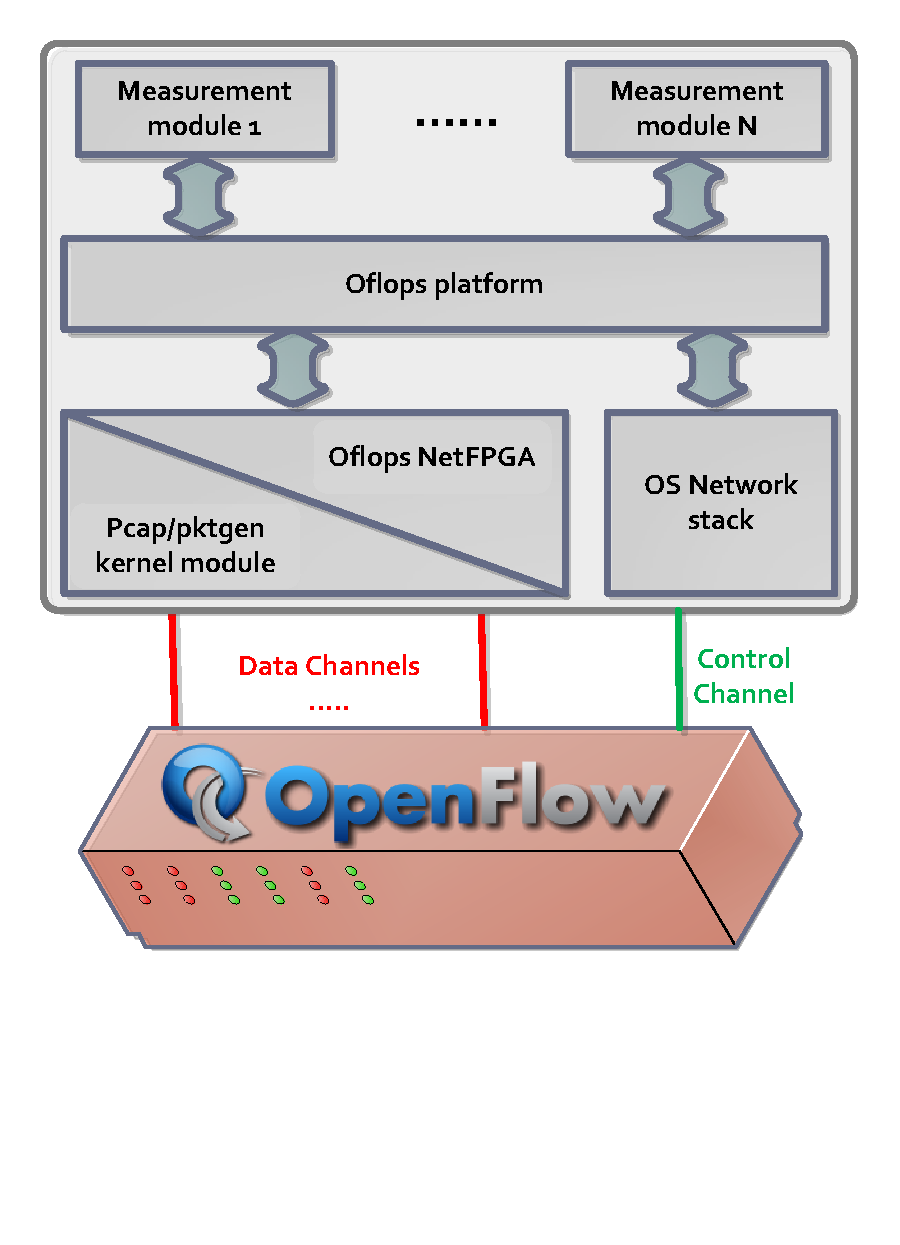
\includegraphics[width=0.99\textwidth]{openflow-design} 
\caption{\oflops design schematic}
\label{fig:oflops_design}
\end{minipage}
\begin{minipage}[b]{0.49\linewidth}
\centering
 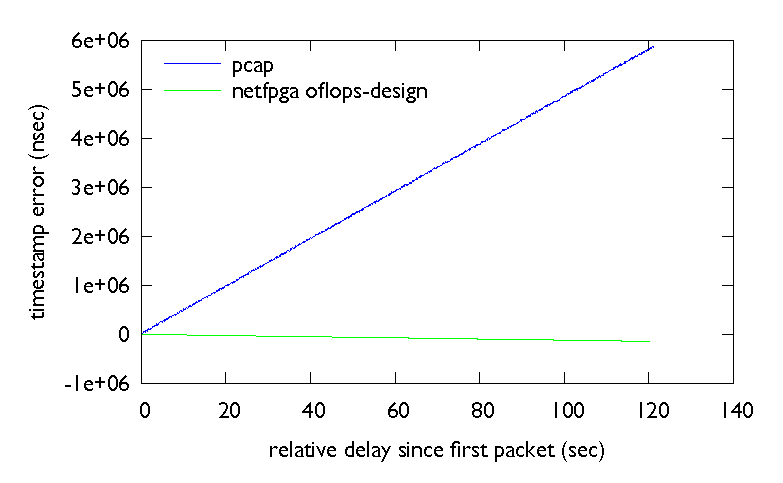
\includegraphics[width=0.99\textwidth]{timer_precision} 
 \caption{Evaluating timestamping precision using a DAG card.}
\label{fig:timestamping}
\end{minipage}
\end{figure}

The \oflops design philosophy aims to develop a low overhead abstraction layer
that allows interaction with an OpenFlow-enabled device over multiple data
channels.  The platform provides a unified system that allows developers to
control and receive information from multiple control sources: data and control
channels as well as SNMP to provide specific switch-state information.
For the development of measurement experiments over \oflops, the platform
provides a rich, event-driven, API that allows developers to handle events
programatically in order to implement and measure custom controller
functionality. The current version is written predominantly in C. Experiments
are compiled as shared libraries and loaded at run-time using a simple
configuration language, through which experimental parameters can be defined.
A schematic of the platform is presented in Figure~\ref{fig:oflops_design}.
Details of the \oflops programming model can be found in the API manual
\cite{oflops-manual}.

The platform is implemented as a multi-threaded application, to take
advantage of modern multicore environments. To reduce latency, our design
avoids concurrent access controls: we leave any concurrency-control complexity 
to individual module implementations. \oflops consists of the following five threads, 
each one serving specific type of events:\\
\textbf{1. Data Packet Generation}: control of data plane traffic generators.\\
\textbf{2. Data Packet Capture}: data plane traffic interception.\\
\textbf{3. Control Channel}: controller events dispatcher.\\
\textbf{4. SNMP Channel}: SNMP event dispatcher.\\
\textbf{5. Time Manager}: time events dispatcher.

\oflops provides the ability to control concurrently multiple data
channels to the switch. Using a tight coupling of the data and control 
channels, programers can understand the impact of the measurement
scenario on the forwarding plane. To enable our platform to run on
multiple heterogeneous platforms, we have integrated support for
multiple packet generation and capturing mechanisms. For the packet
generation functionality, \oflops supports three mechanisms:
user-space, kernel-space through the pktgen module~\cite{pktgen}, and
hardware-accelerated through an extension of the design of the NetFPGA
Stanford Packet Generator~\cite{Covington09}.  For the packet
capturing and timestamping, the platform supports both the pcap
library and the modified NetFPGA design. Each approach provides
different precisions and different impacts upon the measurement
platform.

A comparison of the precision of the traffic capturing mechanisms is 
presented in Figure~\ref{fig:timestamping}. In this experiment we 
use a constant rate 100 Mbps probe of small packets for a two minute 
period. The probe is duplicated, using an optical wiretap with negligible 
delay, and sent simultaneously to OFLOPS and to a DAG card. In the figure, 
we plot the differences of the relative timestamp between each OFLOPS 
timestamping mechanism and the DAG card for each packet. From the figure, 
we see that the pcap timestamps drift by 6 milliseconds after 2 minutes.
On the other hand, the NetFPGA timestamping mechanism has a smaller
drift at the level of a few microseconds during the same period.

% In order to present the precision of each timestamping mechanism, we
% perform a comparison against a DAG card using a 100Mbps packet probe of
% small packet for a monitoring period of 2 minutes (maximum running
% time among all current \oflops modules).  The measurement is contacted
% using an optical wire tap, ensuring traffic duplication with
% negligible delays.  The timestamp differences between each capturing
% mechanism and the dag card are plotted .  In the figure we see that the pcap
% timestamps drift by 6 milliseconds after 2 minutes.
% % while they appear spiky because the percision is on the
% %level of microsends. 
% On the other hand, the NetFPGA timestamping mechanism has a smaller
% precision error at the level of a few microseconds.
%
% \todo{steve: this is why for our purposes we want to have accuracy but we should
% be open and say that depending on the accuracy you really want, how much 
% this really is a problem}
%
% \subsection{old design}
%
%
% We have designed the \oflops\footnote{The \oflops source code is
% made available to the community under an open source license.} 
% tool to assess the performance of OpenFlow
% implementations. The \oflops design-philosophy is to permit an
% abstraction of the interaction with an OpenFlow-enabled device without
% introducing significant additional processing delays.
% % \comment{How much processing delay does \oflops introduce? Just
% %   rought numbers to give an idea...}  \comment{haris: I have this
% %   measurement. I will cover it in the testbed introduction}
% For the development of measurement experiments over \oflops, the
% platform, this version written predominantly in C, provides a rich,
% event-driven, API that allows developers to handle events
% programatically. Experiments are compiled as shared libraries and
% loaded at run-time through a configuration file. The configuration
% file allows the user to define the parameters of the experiment. A
% schematic of the platform is presented in
% Figure~\ref{fig:oflops_design}.  \todo{add a pointer to the \oflops API
%   manual in order to address the claim of how easy it is to develop
%   module for \oflops.}

% In order to assess the performance of a network device that has both
% rich functionality and for which we have little idea of the
% implementation, we require a diverse set of concurrent measurements
% able to encompass all parameters of an experiment. Furthermore,
% to achieve high accuracy across a range of control and measurement
% tasks, we designed a unified platform that permits us to obtain
% information from multiple sources: data and control channels as well
% as SNMP to provide specific switch-state information.

% An OpenFlow controller is the core component of our \oflops framework.
% While OpenFlow controllers like \cite{Gude08,SNAC} provide advanced
% APIs that support fine-grained control of the switch, they do this
% through extensions based upon language mechanisms such as C++ 
% bindings to Python. Such extensions were found to introduce poor 
% performance through added complexity on the control channel, 
% resulting in misleading measurement noise. To further reduce measurement 
% noise, the control flow is configured to provide a path with minimal 
% latency overheads (rather than ones optimised for bulk throughput).

% \oflops provides the ability to control concurrently multiple data
% channels to the switch. By embedding the data channel within the
% platform we are able to understand the impact of the measurement
% scenario on the switching plane. Wanting our platform to run on
% multiple heterogeneous platforms, we have integrated support for
% multiple packet generation and capturing mechanisms. For the packet
% generation functionality, \oflops supports three mechanisms: user-space,
% kernel-space through the pktgen module~\cite{pktgen}, and hardware-accelerated
% through a generator that extends the NetFPGA Stanford Packet
% Generator~\cite{Covington09}.  For the packet capturing and
% timestamping, the platform supports both the pcap library and a
% modified version of the packet capture-functionality from the NetFPGA
% Stanford Packet Generator design. Each approach provides different
% precisions and different impacts upon the measurement platform.
% \todo{steve: this is why for our purposes we want to have accuracy but we should 
% be open and say that depending on the accuracy you really want, how much 
% this really is a problem}

% The \oflops platform currently uses a simple packet generation
% model. Each packet is generated by selecting at random from a uniform
% distribution each value of the header fields from the set of possible
% values that the measurement module defines. The interval between probe
% packets may be selected in a similar fashion although for this paper we use 
% constant intervals. The goal of the \oflops packet generation is not to 
% reproduce the properties of real data traffic; although a module to provide 
% realistic cross-traffic has been tested. For each generated packet we define 
% a custom packet payload: a unique packet-id and a generation-timestamp. 
% By storing this information in the packet, data may be captured and processed 
% offline.

% % For this, we implemented an extra packet markup module in the Stanford Packet Generator hardware design. 

% % \comment{not sure the reader knows what a markup module is...nor how important it is to mention it.}
% % \comment{haris: I was interested to say that the default NF packet
% %   generato doesn't support this by default. I modified a bit the
% %   sentence, but if you think that it is not relevant feel free to
% %   remove it}

% The platform is implemented as a multi-threaded application, to take
% advantage of modern multicore environments. It consists of five
% threads, each one serving specific type of events. To reduce latency
% we have a design that avoids concurrent access controls: we leave any
% concurrency-control complexity to individual module implementations. 
% \oflops contains the following threads:\\
% \textbf{1. Data Packet Generation} a thread to initialize and run the packet probes.\\
% \textbf{2. Data Packet Capture} a thread to capture packets over the data channel
% and transfer them to the measurement module.\\
% \textbf{3. OpenFlow Control Channel} a thread to capture data over the
% control socket, parse their content and generate the appropriate events on the API mechanism.\\
% \textbf{4. SNMP Channel} a thread that monitors passively the SNMP
% channel and collect asynchronous SNMP replies. \\
% \textbf{5. Time Manager} a thread running a high precision event manager where modules can register 
% their own custom events.

% % \begin{enumerate}
% % \item \textit{Data Packet Generation} a thread to initialize and run the packet probes.
% % \item \textit{Data Packet Capture} a thread to capture packets over the data channel 
% % and transfer them to the measurement module.
% % \item \textit{Openflow Control Channel} a thread to capture data over the control socket,
% % parse their content and generate the appropriate events on the API mechanism.
% % \item \textit{SNMP Channel} a thread that monitors passively the SNMP channel and 
% % collect asyncronous SNMP replies.
% % \item \textit{Timer Events} thread, a high precision event thread where modules can 
% % register their own custom events.
% % \end{enumerate}

% % % \Begin{itemize}
% % \item What is the purpose
% % \item 3 threads running in parallel. Separation of task for each
% %   thread.
% % \item what changes occurred in the verilog code of the Stanford
% %   packet generator\cite{Covington09}
% % \item no other hw design provides in parallel packet generation and
% %   packet capturing in parallel.
% % \item we are kinda of during a regression suite which is there to
% %   define performance specifications.
% % \end{itemize}

\section{Measurement setup}\label{sec:oflops-switches}
%
%\todo{Make this a bit more tight to save some space. Need to explain
%why we anonymize the switches. Add a reference to table 2 explaining
%what is show there.}

The number of \of-enabled devices has slowly increased recently, with
switch and router vendors providing experimental \of support such
as prototype and evaluation firmware. At the end of 2009, the \of
protocol specification was released in its first stable version 1.0~\cite{openflow-spec}, 
the first recommended version implemented by vendors for production systems. 
Consequently, vendors did proceed on maturing their prototype implementations, 
offering production-ready \of-enabled switches today. Using \oflops, we 
evaluate \of-enabled switches from three different switch vendors.
Vendor 1 has production-ready \of support, whereas vendors 2 and
3 at this point only provide experimental \of support. 
The set of selected switches provides a representative but not
exhaustive sample of available \of-enabled top-of-rack-style
switching hardware. Details regarding the CPU and the size of the
flow table of the switches are provided in Table~\ref{tbl:switch_list}.

\of is not limited to hardware. The \of protocol reference is the software
switch, OpenVSwitch~\cite{openvswitch}, an important implementation for
production environments. Firstly, OpenVSwitch provides a replacement for the
poor-performing Linux bridge~\cite{bianco10}, a crucial functionality for
virtualised operating systems.  Secondly, several hardware switch vendors use
OpenVSwitch as the basis for the development of their own \of-enabled firmware.
OpenVSwitch development team has standardised a clean abstraction over the
control of the switch silicon (similar to linux HAL), which allows code reuse
over any forwarding entity that implements the switch abstraction. Thus, the
mature software implementation of the \of protocol is ported to commercial
hardware, making certain implementation bugs less likely to (re)appear.  In this
paper, we study OpenVSwitch alongside our performance and scalability study of
hardware switches. Finally, in our comparison we include the \of switch design
for the NetFPGA platform~\cite{openflow-netfpga}. This implementation is based
on the \of reference implementation, extending it with a hardware forwarding
design. 

\begin{table}[h!]
  \begin{center}
{
  \begin{tabular}{ |c | c | c | }
    \hline                        
    \textbf{Switch} & \textbf{CPU} & \textbf{Flow table size} \\
    \hline  
    Switch1 & PowerPC 500MHz & 3072 mixed flows \\
    \hline  
    Switch2 & PowerPC 666MHz & 1500 mixed flows \\
    \hline  
    Switch3 & PowerPC 828MHz & 2048 mixed flows \\
    \hline  
    OpenVSwitch & Xeon 3.6GHz & 1M mixed flows \\
    \hline  
    NetFPGA &  DualCore 2.4GHz & 32K exact \& 100 wildcard \\
    \hline 
  \end{tabular}  

}
\end{center}
\caption{OpenFlow switch details.}
\label{tbl:switch_list}
\end{table}

In order to conduct our measurements, we setup \oflops on a dual-core
2.4GHz Xeon server equipped with a NetFPGA card.
For all the experiments we utilize the NetFPGA-based packet generating and 
capturing mechanism. 1Gbps control and data channels are connected directly 
to the tested switches. We measure the processing delay incurred by the 
NetFPGA-based hardware design to be a near-constant $900$ nsec independent 
of the probe rate.
% In order to define any possible bias introduced by the hardware
% design, we connect two ports of the netfpga card and generate a high
% rate packet probe of small packet. By comparing the generation and
% capture timestamps provided by the platform we measure the delay to
% be constant at 900 nanoseconds.
% This entity contains descriptions of flows, based on the field of
% the openflow tupple, and the actions applied over each matched
% packet. In any openflow-enabled switch there can be numerous flow
% tables with each table having different capabilities. As a general
% rule of thumb, Openflow implementations contain a large software
% table stored in main memory, capable of switching packets at low
% rates, and a smaller h/w based or kernel space table, capable to
% support high rate switching. So far, protocol specifications don't
% define how the switch is expected to allocate flows in flow tables
% and this has led to a diverse set of approaches. Ultimately, the
% goal for an openflow baed application is to keep its large volume
% flows on the fast flow table. Using \oflops we were interested to
% quantify 2 things: the impact of flow manipulation algorithms on the
% switching plane and the scaling properties of the table manipulation
% mechanism. Both of this delays are important when a system has to
% In order to present the capabilities of our tool we develop a set of
% simple experiments using the \oflops platform in order to benchmark
% the perfomance of some simple use case scenarios of the
% protocol. The results of this experiments are presented later in
% Scetion \ref{sec:result}. For our experiment we use four openflow
% implementations which cover a diverse set from available
% implementations. The details of the implementations under test can
% be found in table \ref{tbl:switch_list}. Switch1 and Switch2 are
% hardware switches that support the openflow protocol in their
% firmware. \oflops is installed on a 4 core Intel Xeon server with a
% NetFPGA card. For each switch we connect one of the ports to a
% commodity NIC port of the server, in order to use it as the control
% channel, and 4 other ports to the 4 ports of the NetFPGA card, in
% order to use them as the data channels.
% An important aspect that we noticed during experimentation is the
% fundamental limits that software switches face regarding switching
% performance. Specifically, software switches implement all their
% functionality in the CPU. Because of this, in order for the switch
% to decide the output port for each packet, it has to copy the whole
% packet in main memory. Unfortunately, motherboard buses have limited
% capacity and this may result in packet queueing when the packet rate
% increases. The results of this problem is illustrated in
% Figure~\ref{fig:switch_delay}. In this experiment we are sending a
% single packet probe of small packets and measure the median RTT when
% we increase the packet rate. In the Figure we can see that software
% switches introduce buffering delay on the probe when the packet rate
% icnreases, while hardware accelerated switches can switch packets at
% line rate. Because of this effect we are concious to restrict all
% measurement probes at rates that will not introduce bias during
% comparison.
% \begin{figure}[htb]
%   \begin{center}
%     \includegraphics[width=0.4\textwidth]{graphs/switch_delay/switch-delay}
%   \end{center}
%   \caption{switching delay of implementations}
%   \label{fig:switch_delay}
% \end{figure}
%
% LocalWords: defacto facto virtualised OpenVSwitch Xeon GHz Gb
% NetFPGA Oflops LocalWords: DualCore PowerPC OpenFlow IP VMs


%%%%%%%%%%%%%%%%%%%%%%%%%%%%%%%%%%%%%%%%%%%%%%%
\section{Switch Evaluation}\label{sec:oflops-result}
%%%%%%%%%%%%%%%%%%%%%%%%%%%%%%%%%%%%%%%%%%%%%%%%

% In this section we present a set of tests performed by \oflops to
% measure the behavior and performance of \of-enabled
% devices. These tests target (1) the \of packet processing 
% actions, (2) the update rate of the \of flow table along with 
% its impact on the data plane, (3) the monitoring capabilities provided 
% by \of, and (4) the impact of interactions between different 
% \of operations.

As for most networking standards, there are different ways to implement a
given protocol based on a paper specification. \of is not different in this
regard. The current reference implementation is defined through OpenVSwitch
\cite{openvswitch}. However, different software and hardware implementations may
not implement all features defined in the OpenVSwitch reference, or they may
behave in an unexpected way. In order to understand the behaviour of switch \of
implementation, we develop a suite of measurement experiments to
benchmark the functionality of the elementary protocol interactions.  These
tests target (1) the \of packet processing actions~\ref{sec:result-packets}, (2)
the packet interception and packet injection functionality of the
protocol~\ref{sec:result-pktin}, (3) the update rate of the \of flow table along
with its impact on the data plane,~\ref{sec:result-rate} (4) the monitoring
capabilities provided by \of, and (5) the impact of interactions between
different \of operations.


%As for most networking standards, there are different ways of implementing 
%a given protocol based on a paper specification. OpenFlow is not different in 
%this regard. The current reference implementation is defined through
%OpenVSwitch \cite{openvswitch}. However, different software and hardware
%implementations may not implement all features defined in the
%OpenVSwitch reference, or they may behave in an unexpected way. We
%therefore propose two types of tests within \oflops: feature-oriented
%and performance-oriented. Feature-oriented tests verify which types
%of OpenFlow messages are supported by a given implementation.
%Performance-oriented tests aim to reveal not only the raw performance
%delivered by a given OpenFlow implementation, but also subtle
%interactions between the OpenFlow control plane and the data plane, or
%between different parts of the OpenFlow control plane.

\subsection{Packet modifications}\label{sec:results-packets}

The \of specification \cite{openflow-spec} defines ten packet
modification actions which can be applied on incoming
packets. Available actions include modification of MAC, IP, and VLAN
values, as well as transport-layer fields. A flow definition can
contain any combination of them. The left column of
Table~\ref{tbl:feature_delay} lists the packet fields that can be
modified by an \of-enabled switch.
These actions are used by network devices such as IP routers (e.g.,
rewriting of source and destination MAC addresses) and NAT (rewriting
of IP addresses and ports). Existing network equipment is tailored to
perform a subset of these operations, usually in hardware to sustain
line rate. On the other hand, how these operations are to be used is
yet to be defined for new network primitives and applications, such as
network virtualization, mobility support, or flow-based traffic
engineering.

% Explain how we measure the time taken to perform the modification.
To measure the time taken by an OpenFlow implementation to modify a
packet field header, we generate from the NetFPGA card UDP packets of
100 bytes at a constant rate of 100Mbps (approx. 125 Kpps). 
This rate is high enough to give statistically significant results in
a short period of time, without causing any packet queuing for any of the
switches.  The flow table is initialized with a flow that
applies a specific action on all probe packets and the processing
delay is calculated using the transmission and receipt timestamps,
provided by the NetFPGA.
%, while also low enough so that the impact of
%queuing at the network interface cards can be ignored. 
%Each packet is
%timestamped when leaving the NetFPGA card. The packet then arrives at
%the OpenFlow switch via a direct 1Gbps Ethernet link, the switch
%matches the packet against the flow table, and sends it back to the
%NetFPGA card where it is timestamped again.

\begin{table*}[tb]
\begin{flushleft}
        \begin{tabular}[t]{ |l | c | c | c || c | c | c  || c | c | c | }
          \hline                       
          Mod. type & \multicolumn{3}{|c|}{Switch 1} & \multicolumn{3}{|c|}{ovs} &
          \multicolumn{3}{|c|}{Switch 2} \\ 
          \hline                       
          & med & sd & loss\%  & med & sd & loss\% & med & sd & loss\%\\
          \hline  
          Forward & 4 & 0 & 0 & 35 & 13 & 0& 6 & 0 & 0 \\
          \hline  
          MAC addr. & 4 & 0 & 0 & 35 & 13 & 0& 302 & 727 & 88\\
          \hline  
          IP addr. & 3 & 0 & 0 & 36 & 13 & 0 & 302 & 615 & 88\\
          \hline  
          IP ToS & 3 & 0 & 0 & 36 & 16 & 0 & 6 & 0 & 0\\
          \hline  
          L4 port & 3 & 0 & 0 & 35 & 15 & 0 & 302 & 611 &  88\\
          \hline  
          VLAN pcp & 3 & 0 & 0 & 36 & 20 & 0 & 6 & 0 & 0\\
          \hline  
          VLAN id & 4 & 0 & 0 & 35 & 17 & 0 & 301 & 610 & 88\\
          \hline  
          VLAN rem. & 4 & 0 & 0 & 35 & 15 & 0 & 335 & 626 & 88\\
      \hline
    \end{tabular}
   \begin{tabular}[t]{ |l | c | c | c || c | c | c | }
          \hline                       
          Mod. type & \multicolumn{3}{|c|}{Switch 3} & \multicolumn{3}{|c|}{NetFPGA}\\ 
          \hline                       
          & med & sd & loss\%  & med & sd & loss\% \\
          \hline  
          Forward & 5 & 0 & 0 & 3 & 0 & 0 \\
          \hline  
          MAC addr. & - & - & 100 & 3 & 0 & 0 \\
          \hline  
          IP addr. & - & - &  100 & 3 & 0 & 0 \\
          \hline  
          IP ToS & - & - & 100 & 3 & 0 & 0 \\
          \hline  
          L4 port & - & - & 100 & 3 & 0 & 0 \\
          \hline  
          VLAN pcp & 5 & 0 & 0 & 3 & 0 & 0 \\
          \hline  
          VLAN id & 5 & 0 & 0 & 3 & 0 & 0  \\
          \hline  
          VLAN rem. & 5 & 0 & 0 & 3 & 0 & 0 \\
      \hline
    \end{tabular}
 
\caption{Time in $\mu$s to perform individual packet modifications and packet
loss. Processing delay indicates whether the operation is
  implemented in hardware (\textless10$\mu$s) or performed by the CPU (\textgreater10$\mu$s).}
  \label{tbl:feature_delay}
\end{flushleft}
\end{table*}
% What the table shows...
Evaluating individual packet field modification,
Table~\ref{tbl:feature_delay} reports the median difference between
the generation and capture timestamp of the measurement probe along
with its standard deviation and percent of lost packets.

We observe significant differences in the performance of the hardware
switches due in part to the way each handles packet
modifications. Switch1, with its production-grade implementation,
handles all modifications in hardware; this explains its low packet
processing delay between 3 and 4 microseconds. On the other hand,
Switch2 and Switch3 each run experimental firmware providing only
partial hardware support for \of actions. Switch2 uses the switch
CPU to perform some of the available field modifications, resulting in two orders
of magnitude higher packet processing delay and variance.
Switch3 follows a different approach: All packets of flows with
actions not supported in hardware are silently discarded. The
performance of the OpenVSwitch software implementation lies between
Switch1 and the other hardware switches.  OpenVSwitch fully implements
all \of actions. However, hardware switches outperform
OpenVSwitch when the flow actions are supported in hardware.
% than the delay of the hardware path of the hardware switches,
% dominated by the NIC-CPU latency.
%
% For example, the time of an ensemble of modifications is dictated by the
% maximum time across all modifications.\todo{Last sentence is reported to be
% misleading by the reviewers}
% Furthermore, we notice that for switch1 and openvswitch there is
% limit of 7 actions, which may enveil similrities in the code base.
% From the results presented in Table~\ref{tbl:feature_delay}, we can
% already conclude that an experimental hardware-based OpenFlow
% implementation is likely to deliver poor performance compared to a
% mature software-based implementation running on commodity PC
% hardware

We conducted a further series of experiments with variable numbers of packet
modifications as flow actions. We observed, that the combined processing time of
a set of packet modifications is equal to the highest processing time across all
individual actions in the set. Furthermore, we notice that for Switch1 and 
OpenVSwitch there is a limit of 7 actions, which potentially exposes some
relation in the code base.

\subsection{Traffic interception and injection}\label{sec:results-pktin}

\begin{figure}[ht]
  \begin{center}
    \subfigure[Packet in message latency]
    {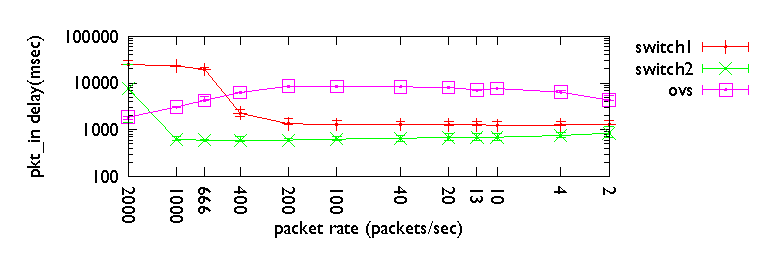
\includegraphics[width=0.99\textwidth]{pkt_in_delay}}
    \subfigure[Packet out message latenct]
	{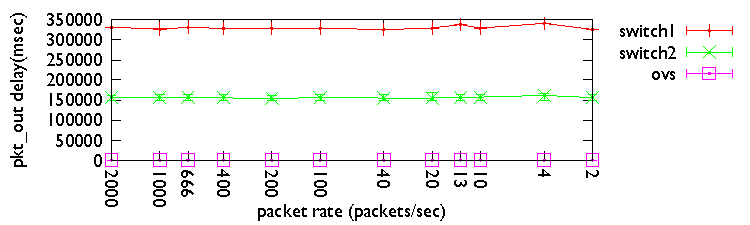
\includegraphics[width=0.99\textwidth]{pkt_out_delay}}
  \end{center}
  \caption{Latency to intercept or inject a packet using the \of protocol}
  \label{fig:pkt_in_out_delay}
\end{figure}

\of protocol permits a controller to intercept or inject traffic over the
control plane. This functionality allowed in the initial design of the \of
controller to be reactive and handle traffic on a per-flow basis. Packet
injection allows the controller to interact with connected network hosts. The
interception mechanism in \of has been reported in the initials deployments of
the protocol to cause significant slow-down in the control plane and led to
switch disconnection at high data rate~\cite{Kobayashi:vn}. This is a direct
consequence of the silicon design in current \of switches, that develop such
functionality as an low-frequency exception mechanism. In order to characterise
this functionality, we develop a simple experiment using \oflops that sends
packets at a specific rate and measure the latency of the switch to process
them. In Figure~\cite{fig:pkt_in_out_delay}, we show the latency induced on
packets both for Packet\_in and Packet\_out messages. We omit in this experiment
Switch 3 as this functionality maxed out its CPU utilisation and after a few seconds
made the switch unresponsive over the control channel. For packet\_out messages,
the switches rate limit through the tcp connection channel the rate of messages
received and as a result they provide a constant performance. For packet\_in
messages, we observe a diverse behaviour between hardware switches at high
packet rates. For Switch 1, packet loss and latency gets high for traffic rates 
above 400 packets per second. Additionally, we noticed that the switch is able to 
process a maximum of 500 packets/sec. For Switch 2 latency and packet loss are 
significantly lower and stable. Switch 2 faced problem to process packet  
important packet at high rates of 2000 packets per second. OpenVSwitch, has a high 
but stable latency for any tested data rates. 

\subsection{Flow table update rate}\label{sec:results-rate}

% So far, we get packet modification primitives and the expected performance that software/hardware can/should deliver.
% 
\begin{figure}[ht]
  \begin{center}
    \subfigure[OpenVSwitch (log-log scale)]
    {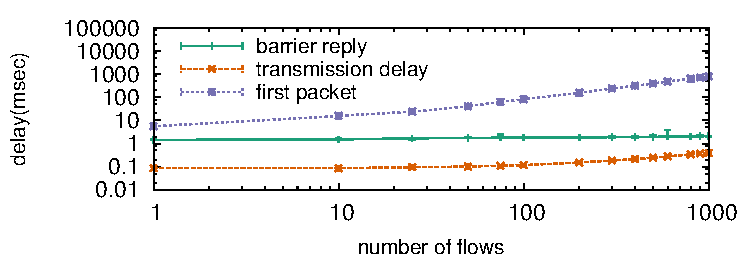
\includegraphics[width=0.99\textwidth]{openvswitch_mod_flow_exact_comparison}}
    \subfigure[Switch1 (log-log scale)]
	{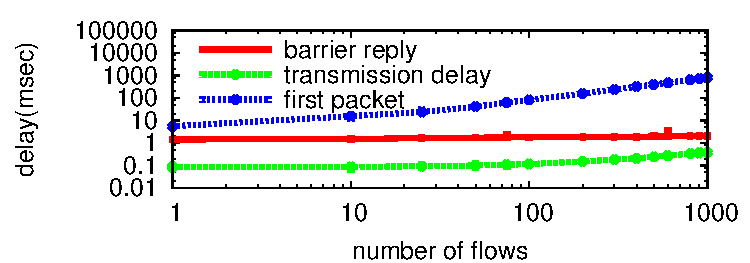
\includegraphics[width=0.99\textwidth]{nec_mod_flow_exact_comparison}}
  \end{center}
  \caption{Flow entry insertion delay: as reported using the
    \texttt{barrier} notification and as observed at the data
    plane.}
  \label{fig:flow_insertion_comparison}
\end{figure}

The flow table is a central component of an OpenFlow switch and is the
equivalent of a Forwarding Information Base (FIB) on routers. Given the
importance of FIB updates on commercial routers, e.g., to reduce the impact of
control plane dynamics on the data plane, the FIB update processing time of
commercial routers provide useful reference points and lower bounds for the time
to update a flow entry on an OpenFlow switch. The time to install a new entry on
commercial routers has been reported in the range of a few hundreds of
microseconds~\cite{shaikh-igp}.

OpenFlow provides a mechanism to define barriers between sets of
commands: the \texttt{barrier} command. According to the OpenFlow
specification~\cite{openflow-spec}, the barrier command is a way to be
notified that a set of OpenFlow operations has been completed. Further, 
the switch has to complete the set of operations issued prior to the barrier 
before executing any further operation. If the OpenFlow implementations 
comply with the specification, we expect to receive a barrier notification for 
a flow modification once the flow table of the switch has been updated, 
implying that the change can be seen from the data plane.

We check the behavior of the tested OpenFlow implementations,
finding variation among them. For OpenVSwitch and Switch1,
Figure~\ref{fig:flow_insertion_comparison} shows the time to install a
set of entries in the flow table. The NetFPGA-based switch results
(not reported) are similar to those of Switch1, while Switch2 and Switch3 
are not reported as this OpenFlow message is not supported by the firmware. 
For this experiment, \oflops relies on a stream of packets of 100 bytes at
a constant rate of 10Mbps that targets the newly installed flows in a
round-robin manner. The probe achieves sufficiently low inter-packet
periods in order to measure accurately the flow insertion time.
%With such a probe stream, we obtain an inter-packet
%period of less than 100$\mu$s, adequate for measuring any change in
%the flow-insertion time.

In Figure~\ref{fig:flow_insertion_comparison}, we show three different
times. The first, {\it barrier notification}, is derived by measuring the time 
between when the \textbf{first insertion command} is sent by the \oflops 
controller and the time the barrier notification is received by the PC. The 
second, {\it transmission delay}, is the time between the first and 
last flow insertion commands are sent out from the PC running \oflops. 
The third, {\it first packet}, is the time between the \textbf{first insertion
 command} is issued and a packet has been observed for the last of
the (newly) inserted rules. For each configuration, we run the
experiment 100 times and Figure~\ref{fig:flow_insertion_comparison}
shows the median result as well as the $10^{th}$ and $90^{th}$ percentiles 
(variations are small and cannot be easily viewed).
%\todo{point that the error
%  bounds are tight and cannot easily viewed on the graph}

From Figure~\ref{fig:flow_insertion_comparison}, we observe that even
though the {\it transmission delay} for sending flow insertion commands 
increases with their number, this time is negligible when compared with 
data plane measurements ({\it first packet}). Notably, the {\it barrier notification} 
measurements are almost constant, increasing only as the transmission delay 
increases (difficult to discern on the log-log plot) and, critically, this operation 
returns before any {\it first packet} measurement. This implies that the way
the {\it barrier notification} is implemented does not reflect the time when 
the hardware flow-table has been updated.

In these results we demonstrate how \oflops can compute per-flow
overheads. We observe that the flow insertion time for Switch1
starts at $1.8$ms for a single entry, but converges toward an
approximate overhead of $1$ms per inserted entry as the number of
insertions grows.

%%%%%%%%%%%%%%%%%%%%%%%%%%%%%%%%%%%%%%%%%%%%%%
\subsubsection*{Flow insertion types}
%%%%%%%%%%%%%%%%%%%%%%%%%%%%%%%%%%%%%%%%%%%%%%

\begin{figure}[h]
  \begin{center}
    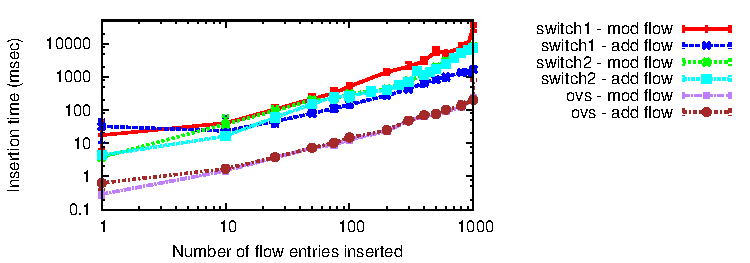
\includegraphics[width=0.80\textwidth]{flow_insertion_delay}
  \end{center}
  \caption{Delay of flow insertion and flow modification, as observed
    from the data plane (log-log scale).}
  \label{fig:flow_insertion_delay}
\end{figure}

We now distinguish between flow insertions and the modification of existing flows.  
With OpenFlow, a flow rule may perform exact packet matches or use wild-cards to 
match a range of values. Figure~\ref{fig:flow_insertion_delay} compares the flow
insertion delay as a function of the number of inserted entries. This is done for the 
insertion of new entries and for the modification of existing entries.

These results show that for software switches that keep all entries in memory, the 
type of entry or insertion does not make a difference in the flow insertion time.
Surprisingly, both Switch1 and Switch2 take more time to modify existing flow entries 
compared to adding new flow entries.  For Switch1, this occurs for more than 10 new 
entries, while for Switch2 this occurs after a few tens of new entries.
After discussing this issue with the vendor of Switch2, we came to the
following conclusion: as the number of TCAM entries increases, updates
become more complex as they typically requires re-ordering of existing
entries.

Clearly, the results depend both on the entry type and implementation.
For example, exact match entries may be handled through a hardware or
software hash table. Whereas, wild-carded entries, requiring support
for variable length lookup, must be handled by specialized memory
modules, such as TCAM. With such possible choices and range of
different experiments, the flow insertion times reported in
Figure~\ref{fig:flow_insertion_delay} are not generalizable, but
rather depend on the type of insertion entry and implementation.

% %%%%%%%%%%%%%%%%%%%%%%%%%%%
\subsection{Flow monitoring}\label{sec:results-monitoring}
% %%%%%%%%%%%%%%%%%%%%%%%%%%%

The use of OpenFlow as a monitoring platform has already been
suggested for the applications of traffic matrix
computation~\cite{opentm-pam,tm-presto} and identifying large traffic
aggregates~\cite{openflow-measurement-hotice}. To obtain direct
information about the state of the traffic received by an OpenFlow
switch, the OpenFlow protocol provides a mechanism to query traffic
statistics, either on a per-flow basis or across aggregates matching
multiple flows and supports packet and byte counters. 
%The result of a query returns packet and byte
%counters, either for the matched flows individually or for the
%aggregate.

We now test the performance implications of the traffic statistics reporting 
mechanism of OpenFlow. Using \oflops, we install flow entries that match 
packets sent on the data path. Simultaneously, we start sending flow statistics 
requests to the switch. Throughout the experiment we record: the delay getting 
a reply for each query, the amount of packets that the switch sends for each 
reply and the departure and arrival timestamps of the probe packets.

Figure~\ref{fig:stat_request} reports the time to receive a flow
statistics reply for each switch, as a function of the request
rate. Despite the rate of statistics requests being modest, quite high
CPU utilization results for even a few queries per second being
sent. Figure~\ref{fig:stat_request} reports the switch-CPU utilization
as a function of the flow statistics inter-request time. Statistics
are retrieved using SNMP. Switch3 is excluded for lack of SNMP
support.

\begin{figure}[h]
  \begin{center}
    \subfigure[Reply time.]
    {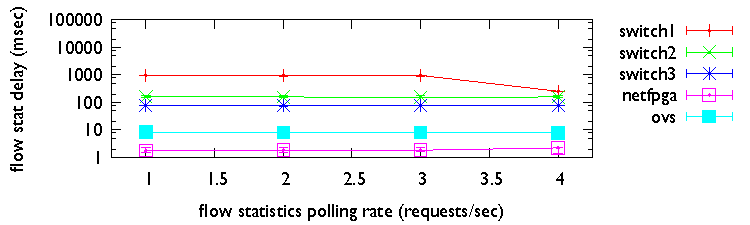
\includegraphics[width=0.99\textwidth]{flow_stats_delay}}
    \subfigure[CPU utilization.]
      {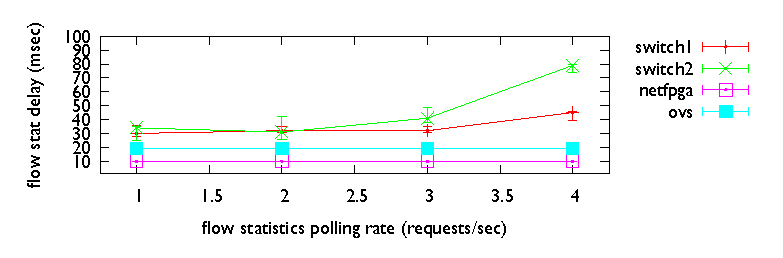
\includegraphics[width=0.99\textwidth]{flow_stats_cpu}\label{fig:stat_request_cpu}}
  \end{center}
  \caption{Time to receive a flow statistic (median) and corresponding CPU utilization.}
  \label{fig:stat_request}
\end{figure}

From the flow statistics reply times, we observe that all switches have (near-)constant 
response delays: the delay itself relates to the type of switch.
As expected, software switches have faster response times than
hardware switches, reflecting the availability of the information in memory
without the need to poll multiple hardware counters. These consistent response
times also hide the behavior of the exclusively hardware switches
whose CPU time increases proportionally with the rate of requests.  We
observe two types of behavior from the hardware switches: the switch
has a high CPU utilization, answering flow-stats requests as fast as
possible (Switch2), or the switch delays responses, avoiding
over-loading its CPU (Switch1). Furthermore, for Switch1,
we notice that the switch is applying a pacing mechanism on its
replies. Specifically, at low polling rates the switch splits its
answer across multiple TCP segments: each segment containing statistics for a
single flow.  As the probing rate increases, the switch
will aggregate multiple flows into a single segment. This suggests that 
independent queuing mechanisms are used for handling flow statistics 
requests. Finally, neither software nor NetFPGA switches see an 
impact of the flow-stats rate on their CPU, thanks to their significantly 
more powerful PC CPUs (Table~\ref{tbl:switch_list}).

%%%%%%%%%%%%%%%%%%%%%%%%%%%%%%%%%%%%%%%%%
\subsection{OpenFlow command interaction}\label{sec:results-interactions}
%%%%%%%%%%%%%%%%%%%%%%%%%%%%%%%%%%%%%%%%%

% why is it important this experiment

An advanced feature of the OpenFlow protocol is its ability to
provide applications with, e.g., flow arrival notifications from the 
network, while simultaneously providing fine-grain control of 
the forwarding process. This permits applications to adapt
in real time to the requirements and load of the
network~\cite{plug_n_serv,Yap09}. Under certain OpenFlow usage
scenarios, e.g., the simultaneous querying of traffic statistics and
modification of the flow table, understanding the behavior of the data
and control plane of OpenFlow switches is difficult without advanced
measurement instrumentation such as the one provided by \oflops. 
%One 
%of the strengths of \oflops is that is enables the development of custom scenarios
%that stress specific aspects of the OpenFlow control or data path.

Through this scenario, we extend Section~\ref{sec:results-rate} to show 
how the mechanisms of traffic statistics extraction and table manipulation 
may interact. Specifically, we initialize the flow table with 1024 exact
match flows and measure the delay to update a subset of 100 flows. 
Simultaneously, the measurement module polls the switch for full table 
statistics at a constant rate. The experiment uses a constant rate 10Mbps 
packet probe to monitor the data path, and polls every 10 seconds for SNMP 
CPU values.

\begin{figure}[t!!]
  \begin{center}
    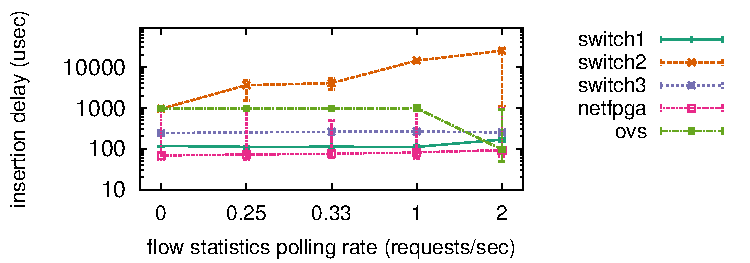
\includegraphics[width=0.99\textwidth]{interaction_test}
  \end{center}
  \caption{Delay when updating  flow table while the controller polls
    for statistics.}
  \label{fig:interaction_test}
\end{figure}

In this experiment, we control the probing rate for the flow statistics 
extraction mechanism, and we plot the time necessary for the modified 
flows to become active in the flow table. For each probing rate, we
repeat the experiment 50 times, plotting the median, $10^{th}$ and 
$90^{th}$ percentile. In Figure~\ref{fig:interaction_test} we can see
that, for lower polling rates, implementations have a near-constant
insertion delay comparable to the results of Section~\ref{sec:results-rate}.
For higher probing rates on the other hand, Switch1 and Switch3 do 
not differ much in their behavior. In contrast, Switch2 exhibits a noteworthy 
increase in the insertion delay explained by the CPU utilization increase
incurred by the flow statistics polling (Figure~\ref{fig:stat_request_cpu}). Finally,
OpenVSwitch exhibits a marginal decrease in the median insertion delay
and at the same time an increase in its variance. We believe this behavior 
is caused by interactions with the OS scheduling mechanism: the constant 
polling causes frequent interrupts for the user-space daemon of the switch, 
which leads to a batched handling of requests.

% \subsection{Timer precision} As part of each flow modification the
% protocol defines that the controller is able to define an expiration
% value for the flow. When a flow is expired, it is removed from the
% table. The protocol supports two different mechanism to define the
% timeout of a flow. Timeouts can be defined either based on the
% insertion time or the last time that the flow was used. The
% definition of the precision of this mechanism would be beneficial to
% applications that require high precision from the routing mechanism.
% In order to address the precision of the mechanism we are developing
% an experiment over the \oflops platform. The experiment utilizes 2
% ports of the switch and a single measurement probe with constant all
% field and random destination IP. During initialization the switch is
% initialized with a single wildcard flow that output packets to port
% 2. At time t=10 sec since the start of the experiment the controller
% sends an ensemble of exact match rules with different destination
% IP's and a hard expiration delay of 10 seconds. All the flows of the
% ensemble contain a single action which outputs packets on port
% 1. The experiments terminate when we receive all the flow expiration
% messages from the switch. During the experiment we log for each flow
% the time at which we received the first and last packet of the
% measurement probe for each destination IP. In the experiment we
% export as a parameter the number of flows send to the switch. For
% each number of flows we rerun the experiment for 20 times. In Figure
% \ref{fig:timer_precision} we present the results of our
% experiment. For each number of flows we plot an errorbar with the
% minimum, maximum and medium of the maximum error in the timeout of a
% flow based on the results of the packet timestamps of the
% measurement probe.
% \subsubsection*{Results}
% \subsection{Simulating a reactive switch} Simulate a Nox like
% behaviour and measure the time send at each stage of the flow
% insertion process. export as parameters the rate we send packets and
% the number of flows inserted.
% \subsubsection*{Results}
% LocalWords:  OpenFlow Oflops IP VLAN balancers SDNs virtualization NetFPGA th
% LocalWords:  UDP Mbps Gbps multiport timestamp OpenVSwitch dev dest src addr

% LocalWords:  NIC ToS TCP pcp interpacket TCAM lookup SNMP CPUs parameterising


\section{\sdnsim introduction} \label{sec:sdnsim-intro}

In the SDN paradigm, backward-compatible evolvability of computer networks is
achieved through the distribution of control to external programmable units. The
protocols provides all required mechanisms in order to allow a remote entity to
get sufficient forward plane feedback and control the forwarding process at a very fine
level. So far the trend in \of design is to aggregate control in a single
control unit, in order to have a single point of control in the network. This
aggregation permits on one hand to achieve higher optimality in forwarding
policy, while on the other hand the logic can be developed in richer
programming environments, than the embedded systems usually found in current
network devices.

The ability to distribute control over multiple functional units, in conjunction
with the complex nature of network stacks, as well as the diverse behaviour of
\of switch and controlling platforms, reduces the ability of developers to
predict the behaviour of an SDN design. In order to reason on correctness,
developers must build realistic small scale experiments, and larger scale 
experiments in order to reason on performance. In the related literature on network
evaluation there have been two main experimental approaches:
\emph{realistic testbed} and \emph{simulation}.

In the realistic experimentation approach, scientists try to reconstruct the
exact properties of the deployment environment. This approach provides an
optimal measurement environment the provides full control of the parameter of
the experiment, but has a significant overhead in resources and configuration
time. Experimenting with a real datacenter would require a high number of
machines that implement full functionality of the target environment, large
interconnection planning and careful metrication and analysis of the resulting
system. These requirements scale badly as the number of network hosts increases.
In order to reduce resource costs, the research community has developed shared
testbeds~\todo{add some pointers.}.  Such testbeds though limit the capability
of users to control measurement noise and network topologies. 

In the simulation approach, researchers replace some part of the functionality
of the system by a simpler model. The goals of such an approach is to reduce the
complexity of the experiment, and achieve scalability for large network sizes. This
approach has two main drawbacks. Firstly, the fidelity of the results depends
extensively on the reality of the assumptions of the model. Secondly, in order to
simulate appropriately the network, the users usually need to rewrite the logic
of their experiments in order to fit the abstraction of the underlying models.
For example, in order to simulate \of-based network currently there is no
off-the-self simulation platform to support the protocol. An \of architect is
required to reimplement its \of logic in order to experiment with architectural
designs. 

\sdnsim~\footnote{\oflops is under GPL licence and can be downloaded from
  \url{http://github.com/crotsos/sdnsim/}} is a novel framework, that bridges
the two domains of experimentation and provides an \of specific development
environment. The framework is written in OcaML, a high performance functional
language, and extends the functionality of the
Mirage~\footnote{\mirageurl} library OS. Developers can
  implement the required functionality of their network design and at the
  compilation step select the target experiment type. \sdnsim provides two
  target options: a simulation target, that runs the Mirage code
  on top of the ns-3 simulation environment, and a realistic target, that build
  and deploys each node of the simulation as a DomU VM and configuration
  resource allocation using xen's API. 

% SDNsim is an ensemble of libraries that provide a simple simulation abstraction
% layer to define and implement SDN deployment scenarios. The platform aims to
% translate network definitions into concrete experiment implementations. More
% specifically, the translation process can generate high-accuracy
% event-driven simulations over the NS3 platform as well as real-time emulation
% by interconnecting DomU virtual machines over the Xen platform.  Here, we
% define the architecture of the platform, describe the library
% applications that the platform supports, provide an initial performance
% evaluation, and conclude with the required functionality. 
% 
% The source code can be found at \url{http://github.com/crotsos/mirage}; it
% has been successfully tested under both Linux and Mac OSX. 
% Details on the required step to install and try the code are forthcoming.
% For Linux, the process is fairly straightforward; 
% for MacOS X, a patch for the NS3 code is required to compile all the required modules. 

\section{Mirage Library OS} \label{sec:mirage-intro}

\begin{figure}
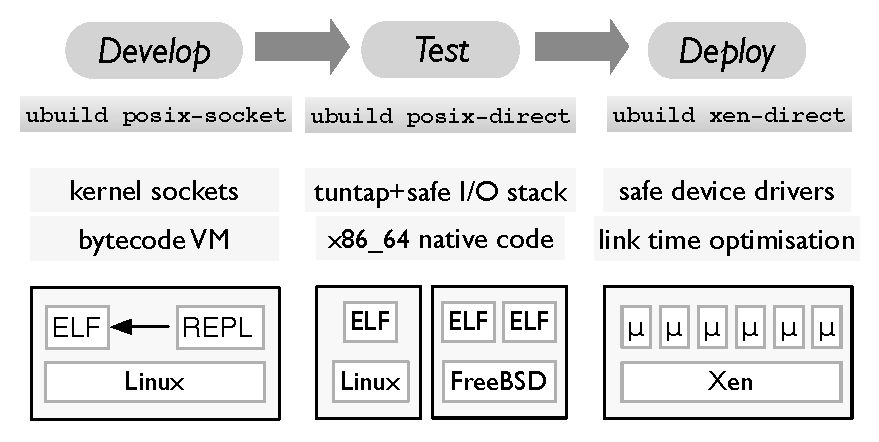
\includegraphics[width=0.9\textwidth]{mirage-toolchain}
\caption{Specialising a \mirage application through recompilation alone, from
  interactive UNIX Read-Eval-Print Loop, to reduce dependency on the host
  kernel, and finally a unikernel VM.}
\label{fig:mirage-toolchain}
\end{figure}

Cloud computing has revolutionized the way the business use IT infrastructures
as well as the way we develop distributed computing applications. The
abstraction is straightforward. A third party entity takes responsibility to
maintain a datacenter. This infrastructure, is partitioned into smaller virtual
computational units which clients can rent in order to run their applications.
The elegance of this model is based on simplicity of the abstraction that the
cloud provider provides to the user and the ability to port existing services
running on a personal computer or a server to the cloud platform. 

Although the simplicity of the exposed abstraction, the cloud architecture
consist of a complex set of processing layers. A single application VM would
include: i) the virtualization runtime layer, ii) the guest OS kernel layer,
iii) A language runtime layer (POSIX, JVM etc.) iv) user-space
thread layer. This layer complexity, although it provides excellent backwards
compatibility for existing datacenter applications, it makes the process of
optimisation, debugging as well as security difficult, while there is a
significant overlap on the functionality provided by each layer. 

Mirage is a clean-slate application synthesis framework that allows users to
compile application to a single bootable VM image. Mirage relies on the idea of
library OS; functionality is separated into logical modules which integrates in
a resulting binary, only if needed by the code. As a result, Mirage is able to
generate small size VM images which additionally are fast to boot. Although, 
OCaml is a functional language, it is able to generate highly performand binary
code and application specific microbenchmarks has shown performance to be
compare to c code implementations. In order to
minimize processing layers, IO operations are coded on top of the NetFront
device abstraction provided by Xen, while the OS is using extensively zero-copy
mechanisms and exposes directly the pages of the shared memory ring to
application space, over a simple abstraction that enforces memory boundaries.

Mirage executes OCaml code over a specialised language runtime modified in two
key areas: memory management and concurrency. Because of the single process
nature of Mirage images, the OS uses a single address space, separated between
the text and data section of the program and the runtime heap. Because the
program code is immutable during runtime, Mirage can lock write access to
executable memory space, thus mitigating buffer overflow attacks. Additionally,
this mechanism removes the requirement of Address Space Randomization (ASR),
which simplifies and makes more efficient memory management.  To provide
concurrency beyond Xen IO polling function, Mirage integrates the Lwt
cooperative threading library~\cite{lwt}. This internally evaluates blocking
functions into event descriptors to provide straight-line control flow for the
developer.  Written in pure OCaml, Lwt threads are heap-allocated values, with
only the thread main loop requiring a C binding to poll for external events.
Mirage provides an evaluator that uses Xen polling to listen for events and wake
up lightweight threads. The VM is thus either executing OCaml code or blocked,
with no internal preemption or asynchronous interrupts. The main thread
repeatedly executes until it completes or throws an exception, and the domain
subsequently shuts down with the VM exit code matching the thread return value.
A useful consequence is that most scheduling and thread logic is contained in an
application library, and can thus be modified by the developer as they see fit. 

In order to provide basic system programming capabilities, Mirage OS provides
two core modules, named Net and OS, that implement and expose the required
functionality for networking and device management, respectively. The API is
similar to the API provided by the Unix model from OCaml; developers can modify
their code and compile existing applications to Mirage VMs. Due to the
simplicity of the OS and Net modules, Mirage provides the ability to compile
code to other target backends, apart from the Xen platform. Specifically, Mirage 
can generate UNIX binaries, using both the POSIX library network functionality 
and raw sockets, and even Javascript executables that run in a browser. There is
also currently an effort to port Mirage in the FreeBSD kernel as well as the
BareboneOS, an assembly written minimum OS. The diverse set
of deployment backends, provides to developers an environment to
test and optimize code gradually. Developers build initially their core logic over
the POSIX backend in order to test the correctness of the code, then they can
try their code over the Mirage default network stack, to perform a small scale
performance evaliation, and finally they can synthesize the resulting deployable 
Xen Image~\ref{fig:mirage-toolchain}.

\section{\sdnsim design} \label{sec:sdnsim-design}

\lstset{language=XML,
numberstyle=\footnotesize,
basicstyle=\ttfamily\footnotesize,
captionpos=b,
}
\begin{lstlisting}[caption={A sample \sdnsim configuration file interconnecting
  a server and a client host},label={lst:sdnsim-conf}]
<?xml version="1.0" encoding="ISO-8859-1"?>
<topology module="Simple_tcp_test" backend="ns3-direct" 
    duration="30">
  <modules>
    <library>lwt</library>
    <library>lwt.syntax</library>
    <library>cstruct</library>
    <library>cstruct.syntax</library>
    <library>mirage</library>
    <library>mirage-net</library>
    <library>pttcp</library>
  </modules>
  <node name="host1" main="host_inner"> 
    <param>1</param>
  </node>
  <node name="host2" main="host_inner"> 
    <param>2</param>
  </node>
  <link src="host1" dst="host2" delay="10" rate="100" 
    queue_size="100" pcap="false"/>
</topology>
\end{lstlisting}

\begin{figure}
\centering
\subfigure[NS3]{
 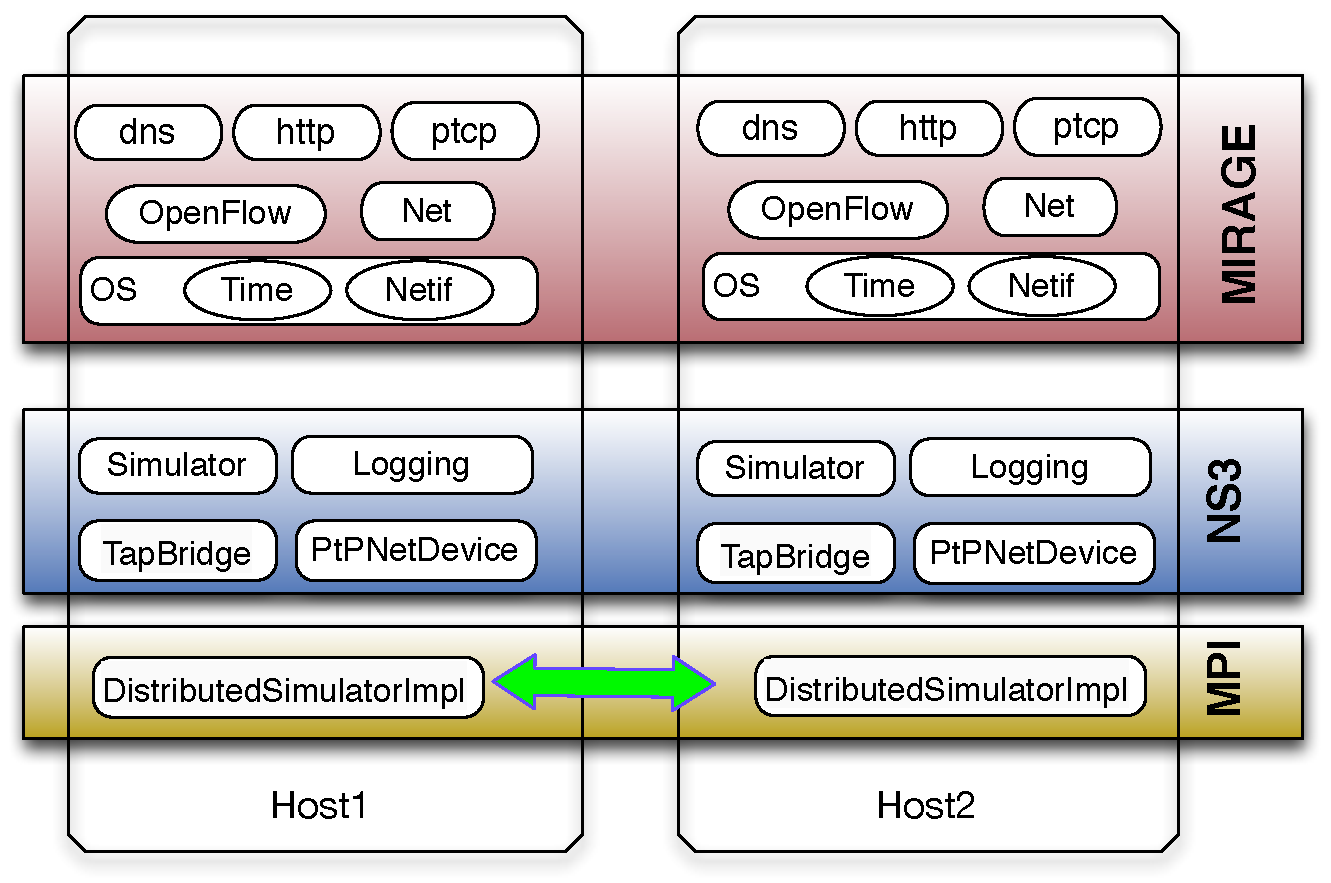
\includegraphics[width=0.45\textwidth]{sdnsim-arch-ns3}
 \label{fig:sdnsim-arch-ns3}}
\subfigure[Xen] {
 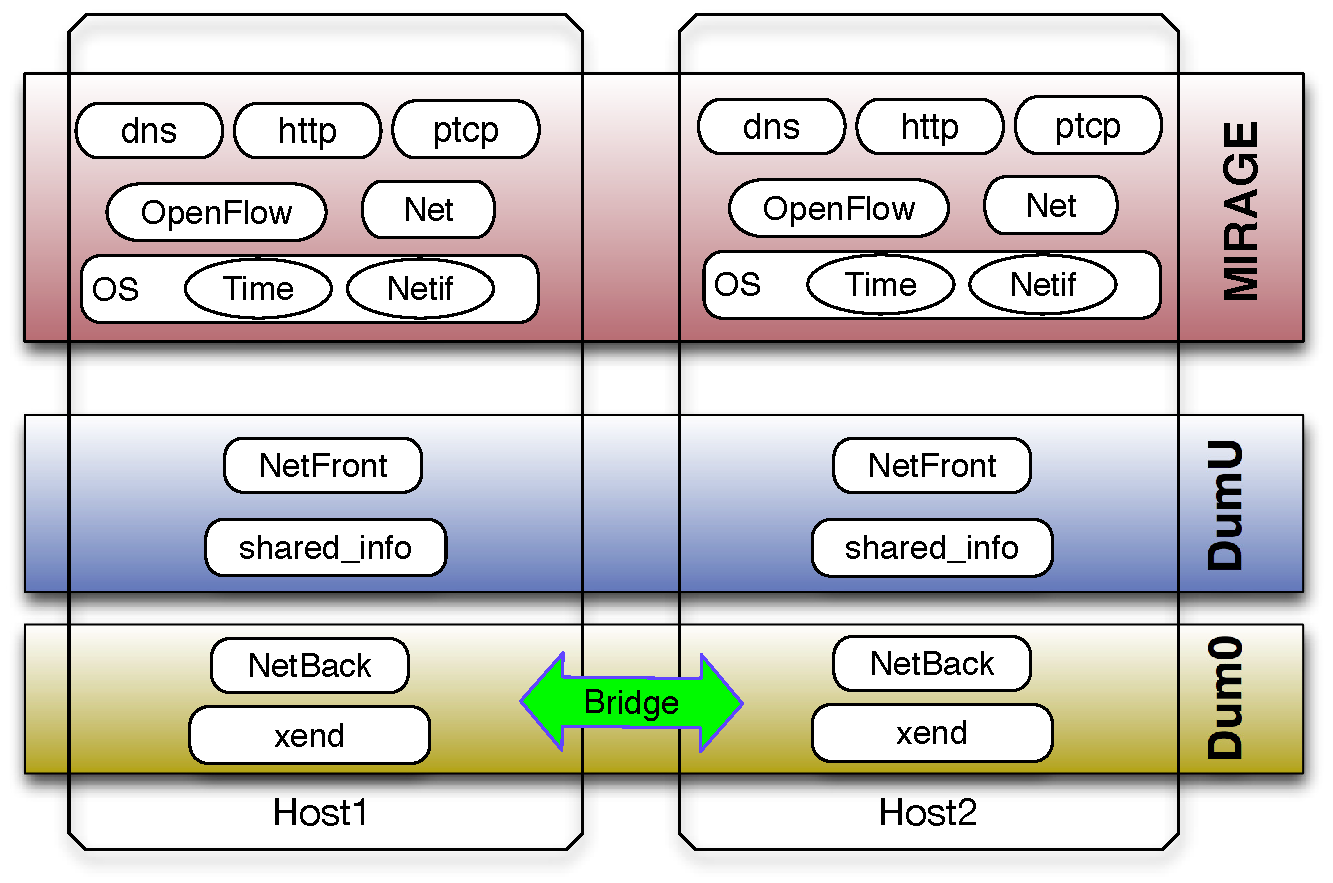
\includegraphics[width=0.45\textwidth]{sdnsim-arch-xen}
 \label{fig:sdnsim-arch-xen}}
\caption{\sdnsim host internal architecture: NS3
  simulation~\ref{fig:sdnsim-arch-ns3} and xen real-time
  emulation~\ref{fig:sdnsim-arch-xen}.}
\label{fig:sdnsim-arch}
\end{figure}

For the user perspective, the core of \sdnsim consists on a single executable
that works as one more OCaml build system. Developers write their OCaml code in
order to define the functionality of network nodes, and use a single xml file in
order to describe the network topology and match functionality to network hosts.
A sample xml file is presented in Listing~\ref{lst:sdnsim-conf}. The
configuration describes a simple client~(host1)~-~server~(host2) configuration.
For an experiment definition, developers needs to define, at minimum,  the core
code module~(topology@module), the target executable~(topology@backend) and the
duration of the experiment~(topology@duration). In order to define a host,
\sdnsim uses a host xml entity. For each host users must define the host
name~(node@name) and the host main function~(node@main), while a number of named
parameters~(node/param) can be passed to the main function. Finally, developers
can define links between hosts~(link@src, link@dst) along with the
device~(link@queue\_size, link@pcap) and propagation properties~(link@rate,
link@delay), using the link xml entity. Links can be used also to integrate
external network interfaces in the simulation, in order to allow the experiment to
interact with entities outside of the experiment scope.

The functionality of a node in the \sdnsim platform can be split in 3 layers.  A
simple representation of the architecture of an \sdnsim host can be seen in
Figure~\ref{fig:sdnsim-arch}.  At the top layer of the host is the application
logic of the host. This layer is defined by the developer, and define the
traffic load of the network and its forwarding logic. In order to allow
realistic traffic patterns, \sdnsim can reuse all the application protocol libraries
supported in the \mirage platform, namely dns, http, ssh and \of. Additionally,
we have re-implemented in OCaml the pttcp tcp test tool functionality~\ref{pttcp},
in order to allow model driven TCP flow generation. 

In the middle layer of the host architecture, we reuse the network library and
the OS abstraction defined by the Mirage platform. These libraries are mapped in
the lower layer of the respective backend. Because this platforms aims to
develop an \of capable simulation platform, the main focus for the integration
between the two lower layer is the fidelity in network functionality and time
consistency. Currently, \sdnsim supports two backends, {\it NS3} and {\it Xen}.
In order to implement the lower layer interaction, a different strategy has been 
followed for each backend. 

\subsection{Xen}

In order to run a Mirage Xen Image, the project provides a simple PV Boot
mechanism. The mechanism initializes a VM with a single virtual CPU, loads the
Xen event channel and jumps to a main function of the VM. The main function
firstly enumerates IO devices and notifies the application and then proceeds to the
main threading scheduling logic. As we have mentioned earlier, the threading
mechanism in Mirage is based on Lwt, a language extension which enables seamless
event-driven asynchronous programming. Using Lwt suntax, each closure can be
noted as blocking, and spawn a new lwt thread. At the lowest level, an lwt
thread is either tied to a blocking IO request, or a time dependent event. Using
this information, the scheduling logic works as follow: If no sleeping thread
is currently available to resume, the schduler calculated the
time left until the next time event and uses it as the timeout parameter for the
IO blocking method (named {\emph domainpoll}) provided by the Xen platform.
Domainpoll registers interest to the respective event handler and ask the Xen
scheduler to put the VM to sleep until either an event occurs or the timeout
option expires.

In order to integrate the clock of a mirage instance with the global clock of
the Xen platform, each time request is mapped to the time counter provided by Xen
shared\_info struct. In respect to the network functionality of Mirage, network
packets are mapped as IO events on the network device of the NetFront driver.
Using this simple logic, users can develop highly functional appliances which
can be deployed as small factor image over the Xen platform.

Further, in order to express network topologies over the Xen platform, 
\sdnsim takes advantage of the Xen API provided by the
latest version of the Xen platform. The API provides the ability to fully
control functionality and resource allocation for each VM running on a Xen
domain. \sdnsim, using the Xen API, is able to implement network 
topologies through vif bridging between hosts, while link
rate and propagation delay can be encoded in the vif definition. 
When \sdnsim  is instructed to run a real-time experiment, it firstly compiles 
all required VM images, creates the appropriate host definition and network
topologies and when the configuration step is completed it can fire the
experiment.

\subsection{NS3}

NS3 is a framework for discrete time packet driven network simulation. It
builds around a basic event-driven simulation engine and provides a set of
libraries that implement an extensive set of network applications, routing
protocols, data-link layer protocols and link emulations models. NS3 is widely
used in academia and is considered as the default simulation tool in the
domain of MANETs and wireless communications. 

Since the way that the NS3 platform is event driven and the scheduling mechanism
is hidden in the Simulation engine, we followed a different approach in order to
map \mirage functionality.
Firstly, in order to bridge the simulation clock with the Mirage host time, we have
mapped the gettimeofday functionality of the OS with the global Simulator
clock of the NS3 platform. Further, in order to provide accurate time events in
the \mirage platform we modified the main mechanism for time events in the
platform, the sleep function. Each sleep call is blocked and scheduled
as an NS3 timed event. The thread is resumed only when the simulator fires the
respective timed event. Finally, in order to make sure that any sleeping thread
is not paused for a long period, the OS schedules {\emph idle} timed events that
check for resume any yielded threads.

% link. We use this connection abstraction because the link state can 
% separated between hosts in order to enable distributed simulations. 

The networking functionality uses the simple link abstraction of a {\emph
  PointToPoint channel}. This model simulates a ppp link over a lossless medium,
a valid model for the full duplex non-shared medium of current network
datacenters. Traffic transmission, uses a single packet queue per network device
shared between the \mirage layer and the NS3 simulator engine.  The only
modification we make on the design of the ns3 link is to modify the network
queue functionality of the network device abstraction. The queue implement a
simple bidirectional feedback mechanism in order to avoid any buffer overflows,
as well as avoid queue polling to check if the queue has space for new packets.
For packet receipt, the NS3 device allows registering receipt callback to each
virtual network device. The packet demuxing callback implements logic to forward
packets to the appropriate listening thread.

% An important assumption of the current architecture that provides accuracy in
% simulation time is the blocking nature of the event-handling process. 
% In this way,
% the virtual clock will not increment while a host is processing an event and
% all processing complexity of hosts is assumed to incur negligible delays. 

A performance limitation that we faced during the development of the NS3 backend
for \sdnsim is the natural inability of the OCaml runtime to support
multi-threaded programming. This simplification provides more predictable
performance for the program, as the garbage collector doesn't have to manage
threads synchronisation, while scalability can be achieved through multiprocess
programs that synchronise through other IPC mechanisms. In order to make \sdnsim
scalable for large network sizes we followed a similar approach. For the
simulation engine we use DistributedSimulationImpl class, which uses message
passing techniques in order to coordinate multiple simulation
instances~\cite{Pelkey:2011ua}. This simulation mechanism uses a simple and
conservative clock synchronisation mechanism, that ensures that all events are
executed in order. 


\section{\sdnsim evaluation} \label{sec:sdnsim-precision}

In order to evaluate the performance of the \sdnsim platform we develop a number
of small scale microbenchmarks in order to evaluate the performance of the \of
protocol functionality as well as the performance of the NS-3 binding.
In~\cite{unikernel}, there is an exhaustive analysis of the performance of the
\mirage platform, which we omit from this section. In Section~\ref{sec:of-perf},
we use two off-the-self \of benchamarking platforms in order to characterise the 
performance of the controller and switch implementation. Further, in
Section~\ref{sec:sdnsim-ns3-perf} we characterise the scalability of the NS3 
backend.

% \subsection{\of library performance} \label{sec:of-perf}

\subsection{\mirage Controller}

We benchmark our controller library's performance through a simple
baseline comparison against two existing OpenFlow controllers, NOX and
Maestro. NOX~\cite{nox} is one of the first and most mature publicly available
\of controllers; in its original form it provides programmability through
a set of Python modules. In our evaluation we compare against both the master
branch and the \emph{destiny-fast} branch, a highly optimised version that
sacrifices Python integration for better performance. Maestro~\cite{maestro}
is an optimised Java-based controller that aims to achieve fairness among
switches. We compare these against the Mirage controller targeting two
different network backends: \emph{mirage-unix} targets the UNIX Sockets
backend and so uses the existing Linux TCP/IP stack, while \emph{mirage-xen}
targets the Xen hypervisor and runs as a domU virtual machine using the Mirage
TCP/IP stack.

Our benchmark setup uses the \emph{cbench}
application\footnote{\url{http://www.openflow.org/wk/index.php/Oflops}}. Each
emulated switch simultaneously generates \emph{packet-in} messages and the
program measures the throughput of the controller in processing these
requests. It provides two modes of operation, both measured in terms of
\emph{packet-in} requests processed per second: \emph{latency}, where only a single
\emph{packet-in} message is allowed in flight from each switch; and
\emph{throughput}, where each switch maintains a full 64\,kB buffer of
outgoing packet-in messages. The first measures the throughput of the
controller when serving connected switches fairly, while the second measures
absolute throughput when servicing requests.
                                                                       
We emulate 16 switches concurrently connected to the controller, each serving
100 distinct MAC addresses. We run our experiments on a 16-core AMD server
running Debian Wheezy with 40\,GB of RAM and each controller configured to use
a single thread of execution. We restrict our analysis to the single-threaded
case as Mirage does not yet support multi-threading. For each controller we
run the experiment for 120\,seconds and measure the per-second rate of
successful interactions. Table~\ref{tbl:controller} reports the average and
standard deviation of requests serviced per second.

Unsurprisingly, due to mature, highly optimised code, \emph{NOX fast} shows
the highest performance for both experiments. However, we note that the
controller exhibits extreme short-term unfairness in the throughput test.
\emph{NOX} provides greater fairness in the throughput test, at the cost of
significantly reduced performance. Maestro performs as well as NOX for
throughput but significantly worse for latency, probably due to the overheads
of the Java VM. Finally, Mirage throughput is somewhat reduced from NOX fast
but substantially better than both NOX and Maestro with both backends; the Xen
backend wins out over the UNIX backend due to reduction of layers in the
network stack. In addition, Mirage Xen achieves the best product of
performance and fairness among all tested controllers in the throughput test.
Comparing latency, both Mirage backends perform much better than Maestro but
suffer somewhat in comparison to NOX: we believe this is due to the lack of
optimisation in the Mirage TCP/IP stack.

\begin{table}\small
\newcommand\T{\rule{0pt}{2.6ex}}
\newcommand\B{\rule[-1.2ex]{0pt}{0pt}}
\centering
\begin{tabular} { l | r@{.}l r@{.}l | r@{.}l r@{.}l }
\hline
\T \multirow{2}{*}{Controller} 
   & \multicolumn{4}{c|}{Throughput (kreq/sec)}  
   & \multicolumn{4}{c}{Latency (kreq/sec)} \\
\B & \multicolumn{2}{c}{avg} & \multicolumn{2}{c|}{std. dev.} 
   & \multicolumn{2}{c}{avg} & \multicolumn{2}{c}{std. dev.} \\
\hline
\T NOX fast   & 122&6 & \quad{} 44&8 & 27&4 & \quad{} 1&4 \\
NOX           &  13&6 &  1&2 & 26&9 & 5&6 \\
Maestro       &  13&9 &  2&8 &  9&8 & 2&4 \\
Mirage UNIX   &  68&1 & 11&7 & 21&1 & 0&2 \\
\B Mirage Xen &  86&5 &  4&4 & 20&5 & 0&0 \\
\hline
\end{tabular}
\caption{\label{tbl:controller}OpenFlow controller performance.}
\end{table}

\subsection{\mirage Switch}

We also use the Oflops benchmark platform~\cite{oflops} to evaluate
performance of the Mirage switch implementation. We compare against the Open
vSwitch\footnote{\url{http://openvswitch.org}}~(OVS) kernel implementation, an
OpenFlow-enabled software switch implemented as a Linux kernel module. OVS is
currently used by many datacenter service providers to enable virtual machines
to be bridged in dom0, while its OpenFlow functionality is used by vendors to
implement OpenFlow firmware.

For this experiment we use two virtual machines, one running the Oflops code,
the other running the OpenFlow switch configured with three interfaces bridged
separately in dom0. One interface provides a control channel for the switch,
while the other two are used as the switch's data channels. This represents a
setup that might be used to enable an application to modify switch
functionality without affecting the network functionality in dom0. Using
Oflops, we generate packets on one of the data channels and receive traffic on
the other, having inserted appropriate flow table entries at the beginning of
the test. We run the test for 30\,seconds using small packets (100\,bytes) and
varying the data rate.

\begin{figure}
\centering
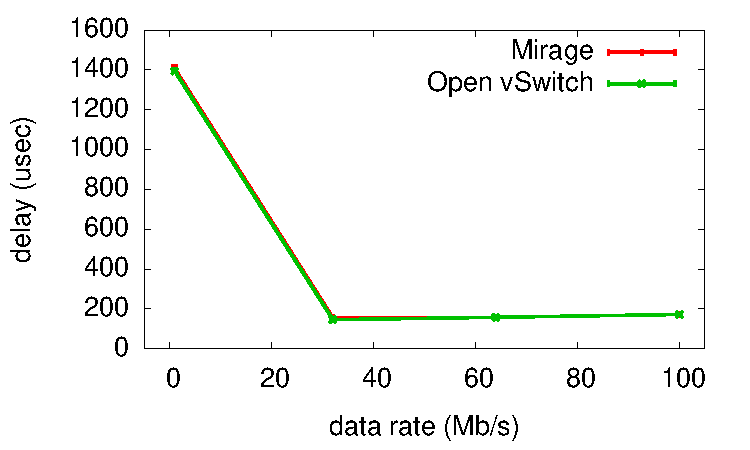
\includegraphics[width=\columnwidth]{switch-media-delay}
\caption{\label{fig:switch}Min/max/median delay switching 100\,byte packets
        when running the Mirage switch and Open vSwitch kernel module as domU
        virtual machines.}
\vspace{-2ex}
\end{figure}

Figure~\ref{fig:switch} plots as error boxes the min, median and max of the
median processing latency of ten test runs of the experiment. We can see that
the Mirage switch's forwarding performance is very close to that of Open
vSwitch, even mirroring the high per-packet processing latency with a probe
rate of 1\,Mb/s; we believe this is due to a performance artefact of the
underlying dom0 network stack. We omit packet loss due to space constraints,
but can report that both implementations suffer similar levels of packet loss.
However, the Mirage switch has a memory footprint of just 32\,MB compared with
the Open vSwitch virtual machine requirement of at least 128\,MB. We are
currently working toward better integration of the Mirage switch functionality
with the Xen network stack to achieve lower switching latency.

\subsection{NS-3 performance} \label{sec:sdnsim-ns3-perf}

In order to test the scaling properties of the NS3 backend we perform a simple
topology experiment~(Figure~\ref{Haris-Fig2}) with variable number of hosts.
The hosts are generated in pairs and are programmed to generate steady-state
full-rate TCP traffic between them.  We use two variations of the topology: A
centralised example where all hosts are  connected to a single switch, and a
localised example, where hosts are distributed between two switches and traffic
is local to the switch.Each switch is connected to an \of controller that
implements a learning switch. The experiment executes 30 seconds of simulation
time.

In Table~\ref{Haris-Table1}, we present the real execution time and the slowdown
factor of each simulation.  The results show that the platform can scale close
to linear the hosts of the simulation create small autonomous partition. In the
centralised example, the \of switch is the bottleneck of the simulation, as it
has to process sequentially all network events. In the distributed example, the
network event processing is distributed between the two switches of the
topology, thus achieving better simulation parallelization.

\begin{figure}
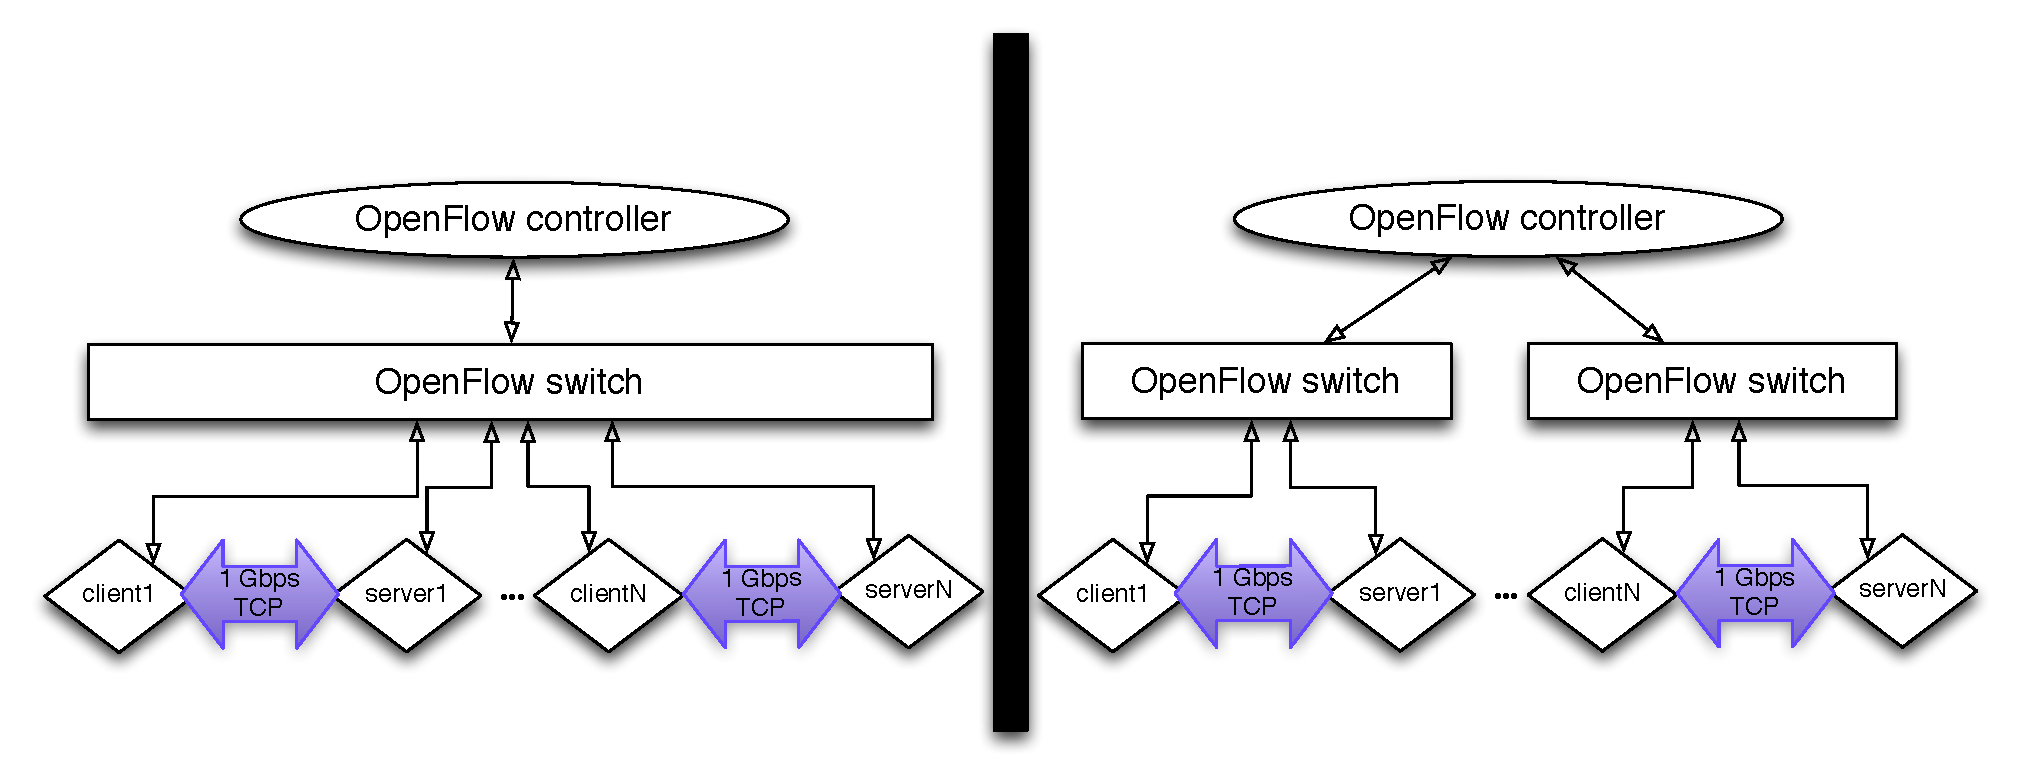
\includegraphics[width=0.9\textwidth]{sdnsim-topology}
\caption{Topology of two basic simulation scenarios for the SDNsim platform}
\label{Haris-Fig2}
\end{figure}

\begin{table}
\label{Haris-Table1}
\begin{center}
\begin{tabular}{|l|c|c|c|c|c|c|} \hline
&\multicolumn{3}{|c|}{Single Switch} & \multicolumn{3}{|c|}{two switches} \\
\cline{2-7}
Number of hosts & 2 & 8 & 12 & 4 & 8 & 12 \\
\hline 
Delay (in min) & 17 & 90 & 171 & 21 &50 & 82 \\
\hline
Slowdown factor & 34 & 180 & 242 & 42 & 100 & 164 \\
\hline 
\end{tabular}
\end{center}
\caption{\sdnsim simulation of a fat-tree topology over NS3 backend allows
  better scaling of the slowdown factor as the traffic is localised. }
\end{table}

\section{Security Tradeoffs on Datacenter Network Micro-control} \label{sec:rdsf-eval}

%%%%%%%%%%%%%%%%%%%%%%%%%%%%%%
\section{Summary and Conclusions}\label{sec:conclusion}
%%%%%%%%%%%%%%%%%%%%%%%%%%%%%%
  
We presented, \oflops, a tool that tests the capabilities and performance of 
OpenFlow-enabled software and hardware switches. \oflops combines advanced 
hardware instrumentation, for accuracy and performance, and provides an extensible 
software framework. We use \oflops to evaluate five different OpenFlow switch 
implementations, in terms of OpenFlow protocol support as well as performance.
%In our performance evaluation, we benchmark the packet processing, flow table
%modification and traffic statistics export functionalities of the switches.

We identify considerable variation among the tested OpenFlow implementations.
We take advantage of the ability of \oflops for data plane measurements to
quantify accurately how fast switches process and apply OpenFlow commands.
For example, we found that the barrier reply message is not correctly implemented,
making it difficult to predict when flow operations will be seen by the data plane.
Finally, we found that the monitoring capabilities of existing hardware switches 
have limitations in their ability to sustain high rates of requests. Further, at high 
rates, monitoring operations impact other OpenFlow commands.

We hope that the use of \oflops will trigger improvements in the
OpenFlow protocol as well as its implementations by various vendors.

%We also readily acknowledge this paper as a snapshot of work in
%progress; every set of results poses new questions but also the role
%of \oflops can evolve as new OpenFlow instantiations are introduced and
%existing ones refined; considerable opportunity exists for future
%work.

% LocalWords:  Oflops OpenFlow

%%% Local Variables: 
%%% mode: latex
%%% TeX-master: "../thesis"
%%% End: 

\chapter{Home network management scalability} \label{sec:homework} 

\ifpdf
\graphicspath{{Chapter2/Chapter2Figs/PNG/}{Chapter2/Chapter2Figs/PDF/}{Chapter2/Chapter2Figs/}}
\else 
\graphicspath{{Chapter2/Chapter2Figs/EPS/}{Chapter2/Chapter2Figs/}} 
\fi

In this chapter we explore the applications of SDN technologies to scale network
control in home networks. Drawing conclusions from existing social and user
studies, we redesign the home network control abstraction to scale management of
the home network. We present a Strawman implementation of a network design which
achieves simplicity and scalability of the control abstraction within the home
environment. Additionally, we propose an extension of our design, which bridges
the gap between the home network users performance requirements and the ISP
resource allocation policy, providing a simple, scalable and user-friendly QoS
mechanism.

In Section~\ref{s:elephant} we present a thorough review of ethnographic and
social studies and elaborate on the nature of the problems and the inherent
opportunities of the specific network environment. In Section~\ref{s:router}, we
describe our home router and how its flow-based approach enables it to help
improve the user experience. In Section~\ref{s:protocols} we present and evaluate
protocol modifications that place the homeowner in more direct control of their
network. In Section~\ref{s:qos} we present a simple QoS policy mechanism that
provides a communication channel between the home owner and the ISP and enables
a user friendly traffic scheduling mechanism for the ISP build using commodity
SDN applications. Finally, in Section~\ref{s:conclusion} we conclude the results of
our exploration.

Note that throughout this Chapter we refer to the individual managing the home
network as the homeowner without loss of generality; clearly any suitably
authorised member of the household, owner or not, may be able to exercise control
based on specifics of the local context. 

% \begin{itemize}
% \item We elaborate on the nature of the problems and opportunities inherent to
%       home networks~(\S\ref{s:elephant});
% \item We describe our home router and how its flow-based approach enables it to
%       help improve the user experience~(\S\ref{s:router}); and
% \item We present and evaluate protocol modifications that place the homeowner in
%       more direct control of their network~(\S\ref{s:protocols}).  
% \end{itemize}

%\mort{explicitly note we do not present user study but tech/infra dev deriving
%from ethno - user study is following in other papers}

% Finally, we present related work~(\S\ref{s:related}) and
% conclude~(\S\ref{s:concl}).  

\section{Technological and Social aspects of home networking} \label{s:elephant}

% Consumer broadband Internet access is a critical component of the digital
% revolution in domestic settings: for example, Finland has made broadband access
% a legal right for all its
% citizens~\footnote{\url{http://www.bbc.co.uk/news/10461048}}. A growing number
% of services are now provided over the Internet, including government,
% entertainment, communications, retail and health.  
The growth of IP enabled devices over the last decade also means many households
are now exploring the use of in-home wired and wireless networking, not only to
allow multiple computers to share an Internet connection but also to enable
local media sharing, gaming, and other applications.  In computer network
literature, a number of studies have been published that highlight the distinct
properties of the home network environment. In
Subsection~\ref{s:home_measurement} we present briefly the connectivity and
traffic mix characteristics of home networks based on the outcome of relevant
studies, while in Subsection~\ref{s:home_social} we discuss the relation of home
networking technologies with the social context of the home, based on relevant
ethnographic studies. Home networking is in parallel a social and a technical
system. These two aspects interrelate dynamically and create an interesting
feedback loop.  

% Despite the growth in Internet use and
% the explosion of interest in home networking, the opacity of networking
% technologies means that they remain extraordinarily difficult for people to
% install, manage, and use in their homes.

% {\it ``The technical know-how required to set up a network and run music or
%   video across cables or wi-fi, is `the elephant in the room that no-one wants
%   to talk
%   about.'\,''}\,\footnote{\url{http://news.bbc.co.uk/1/hi/technology/6949607.stm}}

\subsection{Home Networking as a system} \label{s:home_measurement}

Home networks are highly heterogeneous edge networks, typically
Internet-connected via a single broadband link, where non-expert network
operators provide a wide range of services to a small set of users.  Home
networks use predominanrly ADSL and cable technologies for Internet connectivity, while
int is not uncommon to use fiber, 3g and satellite technologies.
While we focus on home networks, we note that many environments, e.g.,~small
offices, coffee shops, hotels, exhibit similar characteristics and thus may
benefit from similar approaches. Such capabilities are likely to be infeasible
in more traditional settings, e.g.,~backbone and enterprise networks. In this
section we use existing studies to present the technical characteristics of
modern home network. More specifically, we present the type of devices connected to a
home network, the properties of the intra-home-network traffic, as well as, the
Internet traffic and the properties of local and Internet connectivity. 

Recent work on home network characterisation highlights high variability and 
a significant number of connected devices per household. 
% Home network measurement studies have focused both on the local network
% properties as well as the nature of the Internet traffic. Local network analysis
% provides useful insight on the way devices interact within the house and the
% possible performance limitations. Such measurement studies focused mainly on
% developing active or passive measurement tools, that runs on end-hosts in the
% network and collect data. 
In~\cite{homenetProfiler} the authors develop the Homenet measurement framework,
an end-host active measurement tool accompanied by a user survey. The user
survey reports that a home network connects on average 7-8 device, while active
probing discovers on average only 1-2 device active during measurement. Further,
the user survey reports a wide range of connected devices (e.g.~smartphones,
tablets, game consoles, etc.). This points out that the home network hosts a
wide-range of networked devices with diverse operating systems and network
stacks, and any modification in network functionality {\emph must} be backwards
compatible. Additionally, in~\cite{Hatonen10} the authors test a number of
off-the-self home routers and unveil high variability in the semantics of the
NAT and DNS functionality implemented by the router firmware. Nonetheless, since
such routers are widely deployed in home networks, users network behaviour is
resilient to such variability.
% to consider this variability as acceptable. 
% widespread usage of such routing kit, the impact to home networking appears to be
% minimal and home network environment appears to be resilient to non-standard
% router implementations. 

Home networks use predominantly wired and wireless Ethernet technologies to
establish connectivity. Modern PCs provide currently support for both
technologies. Wired network adapters, in their majority, support 802.3ab (1 Gbps
full-duplex) standard and wireless network adapters support predominantly
802.11a/g (54 Mbps) standards with hardware-accelerated encryption, while
802.11n (600 Mbps) standard gains popularity. Modern wired home network
connectivity provides lossless layer-2 transmission, but is less flexible to
accommodate spatial mobility within the household. Wireless technologies are
more user friendly, but their performance is susceptible to environmental
parameters.  The Homenet measurement~\cite{homenetProfiler} study reports than
on the analysed sample wireless signal strength is on average pretty good ($<$
-80dBm). In addition, the wireless card of the measurement PC was able to
receive on average 10 advertisements from nearby wireless networks, a third of
which was using overlapping channel.  Interestingly, these observations point
out the evolution of wireless technology and contrast earlier results
on~\cite{Yarvis05characterizationof}.  The multiple SSID receipt also highlights a
significant access control problem for homeowners.  A wireless network often
reaches beyond the limits of a household.  This problem is usually partially
mitigated using WPA security encryption.  Nonetheless, this policy is crude, as
password knowledge provides full access to the home network and there
isn't a user-friendly mechanism to revoke access.

Home network broadband connectivity has been analysed extensively by the
research community. On a governmental level, official independent authorities
engage in extensive ISP measurement to evaluate the service provided by
broadband providers~\cite{fcc, ofcom}. In~\cite{Dischinger2007}, the authors
contact an active network measurement of residential broadband connections. The
results of the analysis present significant performance differences between ISPs
and pinpoint the performance bottleneck on the last mile of the broadband link.
In~\cite{Sundaresan2011} the authors integrate various measurement mechanisms
into
the home router firmware and contact a long-term performance measurement.  In
their analysis they unveil various differences in ISP performance and measure
the impact of network throttle mechanisms, like PowerBoost~\cite{powerboost}.
The paper points out that broadband performance has multiple factors and cannot
be measurable by a single test, while critical performance factors are
distributed across the network.  Finally, Netalyzer~\cite{Kreibich10}, a
web-based java-applet evaluating network connectivity and protocol openness,
provides useful insight on broadband latency.  Netalyzer, among other tests,
incorporates a network buffer measurement tool, which floods a network path with
packets.  The analysis of the measurement results revealed that network buffer
in the ISP network induce latency of up to 200 msec. 

Home networks also have distinct network traffic properties in comparison to
other network environments.  In~\cite{Reggani12} the authors study the network
traffic from a host point of view for various network environment.  In a home
network setting, hosts generate significant traffic volumes of filesystem and
P2P applications and a large portion of the traffic remains local and is observable
only from within the network.  In terms of the home network Internet traffic
pattern, research has highlighted both significant variability and location-dependence.
In~\cite{Cho2006} authors describe that during the time of their analysis in
Japan there was a significant usage of P2P applications. More recent
studies~\cite{Maier2009} point out that users in Germany have shifted interest
towards web applications and a large portion of traffic is HTTP-based. Similar
results are pointed out in~\cite{Erman2011}, where HTTP flows from an ISP trace
are mapped to application types, and online video and one-click hosting services
appear as the predominant application classes. 

\subsection{Home Network as a social activity} \label{s:home_social}

Home networking technologies have been an interesting domain of study and
application for HCI, Ubiquitous computing and sociology, since it provides an
excellent environment to study the interaction between users and technology.
Studies in the field usually engage in user interviews in order to understand
how users perceive and interact with technology. 

An important aspect in this is understanding how people perceive home network
technologies.
In~\cite{shehanpoole08,grinter05}
the authors ask from home network users to sketch their understanding of the
home network. In the sketch analysis the authors highlight two important
observations; user opacity to the network increases inversely proportional to
their network experience -- establishing  the effectiveness of the deep
abstraction-based design of the current network stack, and users characterize
network devices within the context of the home network. Further,
in~\cite{tolmie07} the authors perform an empirical analysis of the house
members with respect to technology and the home network.  Interestingly, their
finding detect that, on average, users are the least motivated to interact with the
home network in order to optimize it as long as the perceived performance is
tolerable. Additionally, network maintenance is acceptable if it can resemble in
format the other household duties (well defined and simple tasks with short
durations), while the interest conflict that arise due to the shared nature of
some infrastructure is usually solved through negotiation between the household
members. An interesting study on this field is presented in~\cite{Chetty10}. In
this study, the authors develop a visualization system that inform home network
users with statistics on the network bandwidth usage. Interestingly, the
introduction of such a mechanism made users informed on the way the network
functions and how connectivity problems can be traced to network problem or to
other users.  Some users, though, raised privacy concerns for such technologies. 

A number of user studies have augmented the factors that shape home networking
adding as an important factor the design of the building within which the
network is installed. In~\cite{Rodden03} authors describe a 7-layers model
devised by the American writer Stewart Brand in~\cite{Brand94} which
describes how homes evolve architecturally after their initial establishment.
Using this model authors analyse the relationships between Ubquitous
technologies and home design. This study is further focused on the home
networking technologies in~\cite{chetty07}. Authors
contact a user study in order to understand how the home design relates to the
choices of users regarding their home network. The study describes how the user
network decisions are affected by the design of the house, e.g., location of the
network router, while at the same time how the users confuse the limits of the
house with the limits of their network, e.g. users assume that encrypting their
home network is not important since it is contained within the limits of the
house.  In~\cite{rodden04,crabtree03} the
authors study a number of family homes and monitor the real time communications
and the ways in which information is produced and consumer within the house. In
their study they concluide that a lot of these activities have a location
reference within the house, which is related to the involved member as well as
the house planning, while activities can be synthesized as sequences into higher
order activities. Additionally, using these observations, they propose a
framework which can model such interactions. 

Finally, in~\cite{shehan07} authors analyze some common
management and configuration problem in home networks and project them in the
respective design decisions of the network systems.  They present a weight of
evidence that problems with home networking are not amenable to solution via a
`thin veneer' of user interface technology layered atop the existing
architecture.  Rather, they are \emph{structural}, emerging from the mismatch
between the stable `end-to-end' nature of the Internet and the highly dynamic
and evolving nature of domestic environments.  

\todo{add reference to \cite{Mazurek2010} for access control requirements for
  the house.}
% Many empirical studies in recent years have explored the clear mismatch between
% current networking technology and the needs of the domestic setting,  in both
% the
% UK~\cite{}
% and the
% US~\cite{sung07:_my_roomb_rambo,}.
% These studies present a weight of evidence that problems with home networking
% are not amenable to solution via a `thin veneer' of user interface technology
% layered atop the existing architecture.  Rather, they are \emph{structural},
% emerging from the mismatch between the stable `end-to-end' nature of the
% Internet and the highly dynamic and evolving nature of domestic environments.  


\section{Motivations}\label{s:evolution}

\subsection{Home Network: Use cases}

Home networks use the same protocols, architectures, and tools once developed for the
Internet in the 1970s.  Inherent to the Internet's `end-to-end' architecture
is the notion that the core is simple and stable, providing only a semantically
neutral transport service.  Its core protocols were designed for a certain
context of \emph{use} (assuming relatively trustworthy endpoints), made
assumptions about \emph{users} (skilled network and systems administrators both
using connected hosts and running the network core), and tried to accomplish a
set of \emph{goals} (e.g.,~scalability to millions of nodes) that simply do not
apply in a home network. 

In fact, the home network is quite different in nature to both core and
enterprise networks.  Existing studies~\cite{tolmie07,shehan07,shehanpoole08}
suggest domestic networks tend to be relatively small in size with between 5 and
20 devices connected at a time.  The infrastructure is predominately
cooperatively self-managed by residents who are seldom expert in networking
technology and, as this is not a professional activity, rarely motivated to
become expert.  A wide range of devices connect to the home network, including
desktop PCs, games consoles, and a variety of mobile devices ranging from
smartphones to digital cameras.  Not only do these devices vary in capability,
they are often owned and controlled by different household members.  

To illustrate the situation we are addressing, consider the following three
example scenarios, drawn from  situations that emerged from fieldwork 
reported in more detail elsewhere~\cite{wmust2011,Chetty10}: 
 
\textbf{Negotiating acceptable use}.  {\it William and Mary have a spare room
  which they let to a lodger, Roberto.  They are not heavy network users and so,
  although they have a wireless network installed, they pay only for the lowest
  tier of service and they allow Roberto to make use of it.  The lowest tier of
  service comes under an acceptable use policy that applies a monthly bandwidth
  cap.  Since Roberto arrived from Chile they have exceeded their monthly cap on
  several occasions, causing them some inconvenience.  They presume it is
  Roberto's network use causing this, but are unsure and do not want to cause
  offence by accusing him without evidence.}

\textbf{Welcome visitors, unwelcome laptops}.  {\it Steve visits his friends
  Mike and Elisabeth for the weekend and brings his laptop and smartphone.  Mike
  has installed several wireless access points throughout his home and has
  secured the network using MAC address filtering in addition to WPA2.  To
  access the network, Steve must not only enter the WPA2 passphrase, but must
  also obtain the MAC addresses of his devices for Mike to enter on each
  wireless access point.  Steve apologizes for the trouble this would cause and,
  rather than be a problem to his hosts, suggests he reads his email at a local
  cafe.} 

\textbf{Sharing the medium socially efficient}.  {\it Richard is the teenage son
  of Derek and has a great interest in Music, downloading a lot of music from the
  Internet. Derek works some times in the night from home using the Terminal
  Services provided by his company. Tension is created between them as Derek
  blames Richard downloading activity for his poor performing remote desktop
  application. } 

In such ways, simple domestic activities have deep implications for
infrastructures that generate prohibitive technical overheads.  In the first
scenario, the problem is simply that the network's behaviour is opaque and
difficult for normal users to inspect; in the second, the problems arise from
the need to control access to the network and the technology details exposed by
current mechanisms for doing so.  

Home networks enable provision of a wide range of services, e.g.,~file stores,
printers, shared Internet access, music distribution.  The broad range of
supported activities, often blending work and leisure, make network use very
fluid.  In turn, this makes it very hard to express explicitly \emph{a priori}
policies governing access control or resource management~\cite{tolmie07}.
Indeed, fluidity of use is such that access control and policy may not even be
consistent, as network management is contingent on the household's immediate
needs and routines.

\subsection{Home Networks: Revolution!} \label{s:revolution}

Current network functionality is spread across multiple layers that implement
different abstractions, while multiple protocols are used to allow network hosts
to communication over these layers. Each layer exposes a different set of
control parameters and effective network management \emph{must} exercise control
on multiple layers. Ultimately, this control distribution architecture is not
scalable for the average user. Simply creating a user interface layer for the
existing network infrastructure will only reify existing problems.  Rather, we
need to investigate creation of new network architectures reflecting the
socio-technical nature of the home by taking into account both human and
technical considerations. Control of the network can be redefined, exposing only
the required control and semantically appropriate abstraction, in order to scale
controllability of the network.  
% For example, we
% may need to explore architectures that sacrifice scalability in favor of
% installability, evolvability, and maintainability.  

To this end we exploit local characteristics of the home: devices are often
collocated, are owned by family and friends who physically bring them into the
home, and both devices and infrastructure are physically accessible.
Essentially, the home's physical setting provides a significant source of
heuristics we can understand, and offers a set of well understood practises that
might be exploited in managing the infrastructure.  

We exploit human understandings of the local network and the home to guide
management of the supporting
infrastructure~\cite{crabtree03} by focusing on the
home router not only as the boundary point in an edge network but as a physical
device which can be exploited as a point of management for the domestic
infrastructure.  Within our router, we focus on flow management for three
reasons: 

\begin{itemize}
    \item we do not require forwarding scalability to the same degree as the
          core network; 
    \item doing so allows us to monitor traffic in a way that is more meaningful
          for users; and 
    \item we can apply per-flow queueing mechanisms to control bandwidth
          consumption, commonly requested by users.  
  \end{itemize}
%% \mort{distinction is now being pushed as: large-scale networks focus
%%      on packets not flows for scalability (plus other things of
%%      core/enterprise nets); we go for flows and explore impact of this
%%      decision} 

%% \mort{focusing on flows lets us (a) monitor traffic in a way that's
%%      (somewhat) meaningful for users (but cf.  wmust); (b) control
%%      traffic using a range of standard mechanisms such as per-flow
%%      queueing/qos} 

\section{Reinventing the Home Router} \label{s:router}
 
\begin{figure} 
  \centering 
  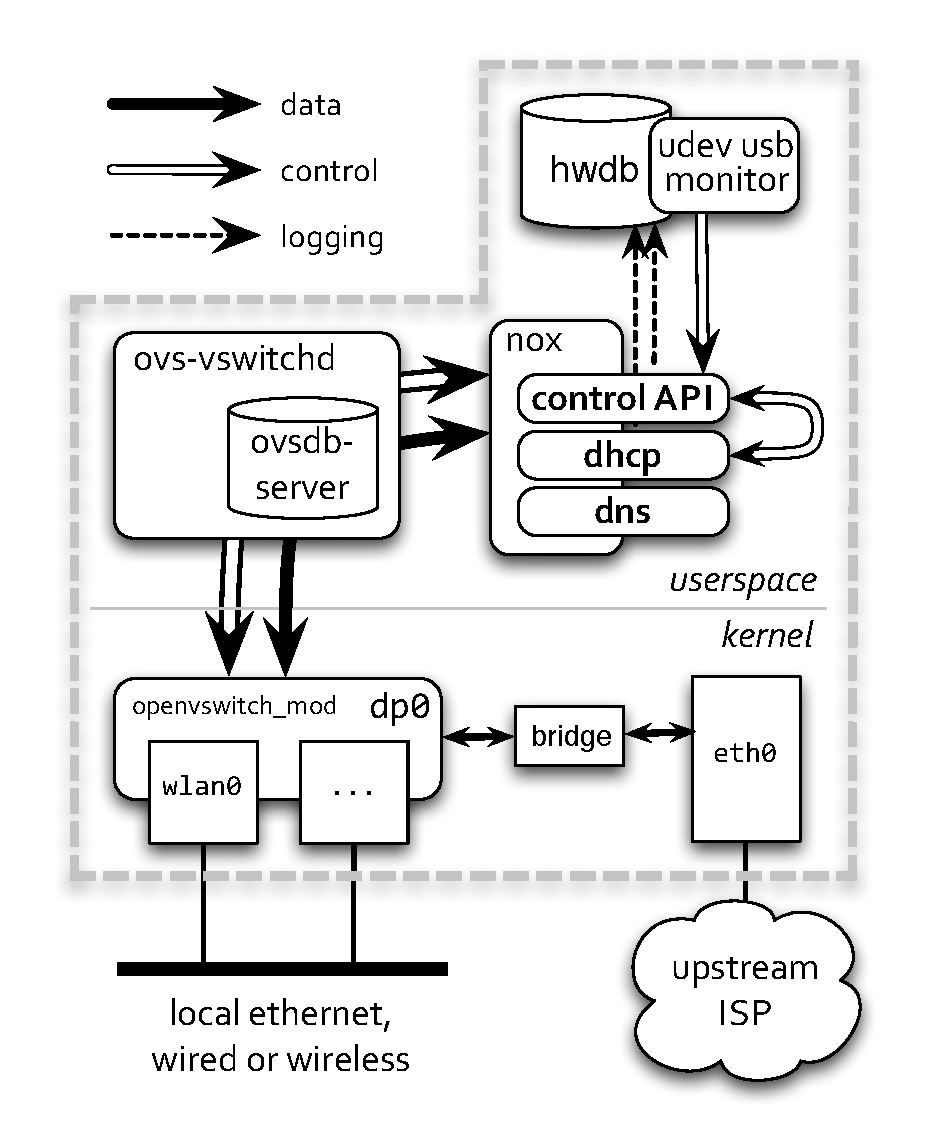
\includegraphics[trim=0.5cm 1cm 0.5cm 2.5cm, width=0.5\columnwidth]{architecture}
  \caption{\label{f:architecture}Home router architecture.  \ovs
    (\emph{ovs*}) and NOX manage the wireless interface.  Three NOX modules
    provide a web services control API, a DHCP server with custom address
    allocation and lease management, and a DNS interceptor, all logging to the
    Homework Database (\emph{hwdb}) (\S\ref{s:protocols}). 
}\end{figure}

Our home router is based on Linux 2.6 running on a micro-PC
platform.\footnote{An Atom 1.6GHz eeePC 1000H netbook with 2GB of RAM running
  Ubuntu 10.04.} Wireless access point functionality is provided by the
\emph{hostapd} package.  The software infrastructure on which we implement our
home router, as shown in Figure~\ref{f:architecture}, consists of the \ovs \of
implementation, a NOX controller exporting a web service interface to control
custom modules that monitor and manage DHCP and DNS traffic, plus the Homework
Database~\cite{sventek11:_infor_plane_archit_suppor_home_networ_manag} providing
an integrated network monitoring facility.  This gives us a setup very similar
to a standard operator-provided home router where a single box acts as wireless
access point, multiplexes a wired connection for upstream connectivity to the
ISP, and may provide a small number of other wired interfaces. 
                                                                    
We next describe the main software components upon which our router relies.
Using this infrastructure, we provide a number of novel user interfaces, one of
which we describe briefly below; details of the others are available
elsewhere~\cite{mortier11:_suppor_novel_home_networ_manag}.  Note that a key
aspect of our approach is to avoid requiring installation of additional
software on client devices: doing so is infeasible in a home context where so
many different types of device remain in use over extended periods of time.

\subsection{\of, \ovs \& NOX} \label{s:openflow}

We provide \of support using \ovs~\cite{openvswitch}, \of-enabled switching
software that replaces the in-kernel Linux bridging functionality able to
operate as a standard Ethernet switch as well as providing full support for the
OpenFlow protocol.  We use the NOX~\cite{nox} controller as it provides a
programmable platform abstracting OpenFlow interaction to events with associated
callbacks, exporting APIs for C++ and Python.

Our network control logic, discussed in Section~\ref{s:protocols}, is implemented
over the NOX controller abstraction and split between 5 different modules. The
C++ module {\it hwdb} synchronizes router state with the hwdb home database,
presented in Section~\ref{s:hwdb}, the C++ module {\it homework\_dhcp}
implements our custom DHCP server, the C++ module {\it homework\_routing}
implements the forwarding logic of the design, the C++ module {\it homework\_dns}
implements the DNS interception functionality and the Python module {\it
  homework\_rpc} exposes the control API as a Web service. 

\begin{table}
  \begin{tabular} {p{0.35\columnwidth}p{0.55\columnwidth}} 
    \textbf{Method} & \textbf{Function} \\ 
    \url{permit/<eaddr>} & Permit access by specified client\\ 
    \url{deny/<eaddr>} & Deny access by specified client\\
    \url{status/[eaddr]} & Retrieve currently permitted clients, or status of specified client \\ 
    \url{dhcp-status/} & Retrieve current MAC--IP mappings\\
    \url{whitelist/<eaddr>} & Accept associations from client\\
    \url{blacklist/<eaddr>} & Deny association to client\\
    \url{blacklist-status/} & Retrieve currently blacklisted clients\\
    \url{permit-dns/<e>/<d>} & Permit access to domain \texttt{d} by client \texttt{e}\\ 
    \url{deny-dns/<e>/<d>} & Deny access to domain \texttt{d} by client \texttt{e}\\ 
  \end{tabular} 
  \caption{\label{t:api}Web service API;
    prefix all methods \texttt{https://.../ws.v1/}.  $<$\,$X$\,$>$ and $[X]$
    denote required and optional parameters.}
\end{table}

Our router provides flow-level control and management of traffic via a single
\of datapath managing the wireless interface of the platform.\footnote{Without
  loss of generality, our home router has only a single wired interface so the
  only home-facing interface is its wireless interface; other home-facing
  interfaces would also become part of the \of datapath.} 
  % We provide NOX
  % modules that implement a custom DHCP server, control forwarding, control
  % wireless association via filtering, and intercept DNS lookups.  
Control of the router is provided via a simple web service (Table~\ref{t:api}).
Traffic destined for the upstream connection is forwarded by the datapath for
local processing via the kernel bridge, with Linux's \emph{iptables} IP
Masquerading rules providing standard NAT functionality.\footnote{While NAT
  functionality could be implemented within NOX, it seemed neither interesting
  nor necessary to do so.}

%% Without loss of generality, the device we describe in this paper has
%% only a single wired interface so the only home facing interface is its
%% wireless interface, and this is the physical interface managed by the
%% OpenFlow datapath.

\subsection{The Homework Database} \label{s:hwdb}
 
%% \mort{reduce this- it's reported elsewhere: it's a streaming database,
%%  collecting ip layer supporting rpc interaction, and defaults to providing
%%  a Flows table among others; provides the basic measurement
%%  facility accessed by the many uis via rpc}
 
In addition to \ovs and NOX we make use of the Homework Database,
\emph{hwdb}, an active, ephemeral stream
database~\cite{sventek11:_infor_plane_archit_suppor_home_networ_manag}.  The
ephemeral component consists of a fixed-size memory buffer into which arriving
tuples (events) are stored and linked into tables.  The memory buffer is treated
in a circular fashion, storing the most recently received events inserted by
applications measuring some aspect of the system.  The primary ordering of
events is time of occurrence.  

The database is queried via a variant of CQL~\cite{arasu05:_cql} able to express
both temporal and relational operations on data, allowing applications such as
our user interfaces to periodically query the ephemeral component for either raw
events or information derived from them. 
Applications need not be collocated on the router as \emph{hwdb} provides a
lightweight, UDP-based RPC system that supports one-outstanding-packet semantics
for each connection, fragmentation and reassembly of large buffers, optimization
of ACKs for rapid request/response exchanges, and maintains liveness for
long-running exchanges.  Monitoring applications request can execute temporal
query on specific types of events.  \emph{hwdb} also provides notification
functionality; applications may register interest in \emph{future} behaviour
patterns and receive notification when such patterns occur in the
database.  The work described in this paper makes use of three tables:
\emph{Flows}, accounting traffic to each 5-tuple flow; \emph{Links}, monitoring
link-layer performance; and \emph{Leases}, recording mappings assigned via DHCP.

%% By default, there are three tables, Flows, Links, and Leases.  Table
%% Flows stores the number of packets and bytes as observed (inserted) by
%% an application that accumulates these counts for each 5-tuple flow per
%% measurement interval (currently set to 1s in our deployments).  In a
%% similar manner, table Links stores the average RSSI, the number of
%% packets, the number of bytes, and the number of retransmissions
%% observed for each wireless device identified by its MAC
%% address.  Finally, table Leases stores any actions taken by the DHCP
%% server (e.g., granting or revoking a lease) with the mappings between
%% allocated IP addresses and host MAC addresses and names.  

%% \mort{fix link para}

%% We next describe details, implementation and evaluation of the two
%% strategies by which we exploit the home network context.  First we
%% consider the ways in which people may be more directly involved in
%% infrastructure protocols.


\subsection{The Guest Board} \label{s:guest-board}

% \mort{explicitly tie to ethno story} 

\begin{figure} 
  \centering 
  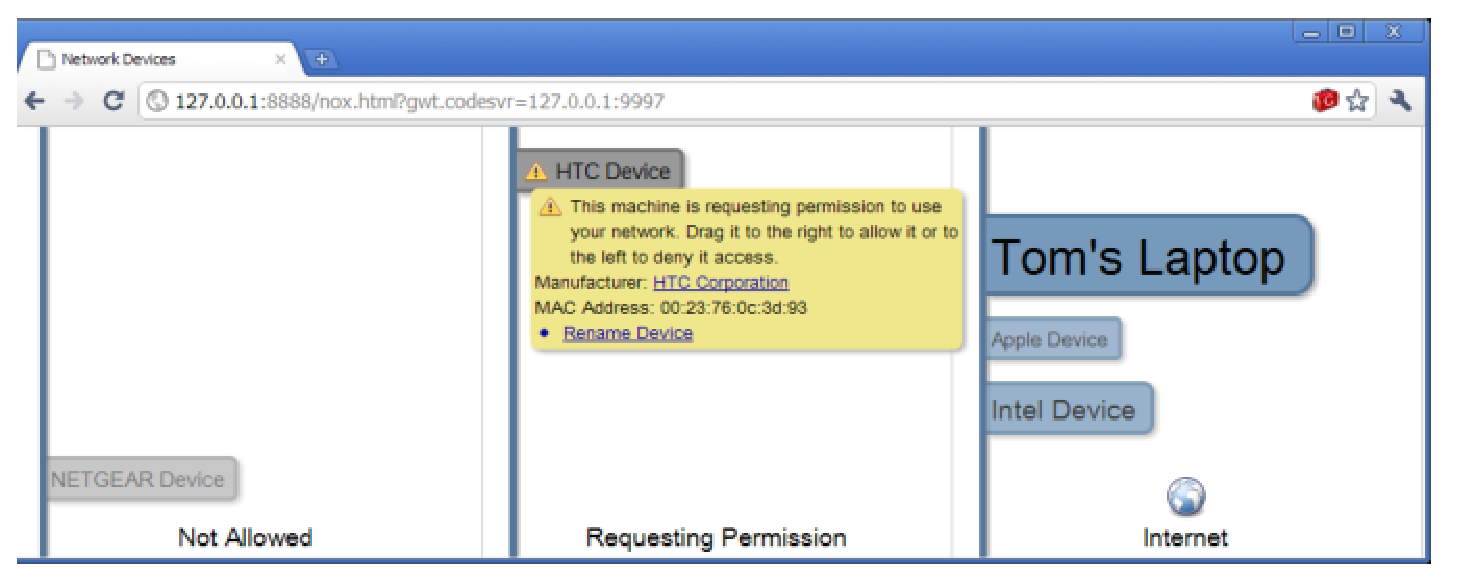
\includegraphics[width=0.9\columnwidth]{homework_guest_board}
  \caption{\label{f:guest-board}The \emph{Guest Board} control panel, showing an
    HTC device requesting connectivity.}
\end{figure}

This interface exploits people's everyday understanding of control panels in
their homes, e.g.,~heating or alarm panels, to provide users with a central
point of awareness and control for the network. We exploit this physical arrangement to
provide a focal point for inhabitants to view current network status and to
manage the network.  It provides a real time display of the current status of
the network (Figure~\ref{f:guest-board}), showing devices in different zones
based on the state of their connectivity.  The display dynamically maps key
network characteristics of devices to features of their corresponding labels.
Mappings in the current display are: 

\begin{itemize}
\item Wireless signal strength is mapped to device label transparency, so
      devices supplying weak signals fade into the background.
\item Device bandwidth use is proportional to its label size, e.g.,~Tom's Laptop
      in Figure~\ref{f:guest-board} is currently the dominant bandwidth user. 
\item Wireless Ethernet retransmissions show as red highlights on the device's
  label, indicating devices currently experiencing wireless reliability problems. 
\end{itemize}

Devices in range appear on the screen in real-time, initially in the leftmost
panel indicating they are within range of the home router but not connected.
The central panel in the control displays machines actively seeking to associate
to the access point. This zone exploits the underlying strategy of placing
people in the protocol discussed in Section~\ref{s:protocols}.  When devices
unknown to the network issue DHCP requests, the router's DHCP server informs the
guest board and a corresponding label appears in this portion of the display.
If a user wishes to give permission for the machine to join the network they
drag the label to the right panel; to deny access, they drag the label to the
left panel. The guest board provides both a central control point and, by
drawing directly upon network information collected within our router, a
network-centric view of the infrastructure. 

% The guest board provides both a central control point and, by drawing directly
% upon network information collected within our router, a network-centric view of
% the infrastructure.  The interface is implemented in HTML/CSS/Javascript
% allowing it to be displayed on a range of devices, currently under trial with
% users.  The router's measurement and control APIs described above are also being
% used to build a wide range of other interfaces for use via smartphones, web
% browsers, and custom display hardware.

%% \mort{...it is just one of several interfaces we have built that use
%%  the features of our home router, ranging from network artefacts
%%  to phyiscally mediated access via usb key tokens; see uist2011
%%  paper insub for details}

\section{Putting People in the Protocol} \label{s:protocols}

%\mort{note that this is tied to social convention of home visiting, network
%part of the home not separate to it, etc}
We use our home router to enable \emph{ad hoc} control of network policy by
non-expert users via interfaces such as the Guest Board
(Figure~\ref{f:guest-board}).  This sort of control mechanism is a natural fit
to the local negotiation over network access and use that takes place in most
home contexts.  While we believe that this approach may be applicable to other
protocols, e.g.,~NFS/SMB, LPD, in this section we demonstrate this approach via
our implementation of a custom DHCP server and selective filters for wireless
association and DNS that enable management of device connectivity on a
per-device basis. 

Specifically, we describe and evaluate how our router manages IP address
allocation via DHCP, two protocol-specific (EAPOL and DNS) interventions it
makes to provide finer-grained control over network use, and its forwarding
path.  We consider three primary axes: \emph{heterogeneity} (does it still
support a sufficiently rich mix of devices); \emph{performance} (what is the
impact on forwarding latency and throughput of our design and implementation
decisions); and \emph{scalability} (how many devices and flows can our router
handle).  In general we find that our home router has ample capacity to support
observed traffic mixes, and shows every indication of being able to scale beyond
the home context to other situations, e.g., small offices, hotels. 

\subsection{Address Management} \label{s:addresses}

DHCP~\cite{rfc:2131} is a protocol that enables automatic host network
configuration. It is based on a four way broadcast handshake that allows hosts
to discover and negotiate with a server their connectivity parameters.  As part
of our design we extend the functionality of the protocol to achieve two goals.
First, we enable the homeowner to control which devices are permitted to connect
to the home network by interjecting in the protocol exchange on a case-by-case
basis.  We achieve this by manipulating the lease expiry time, allocating only a
short lease (30s) until the homeowner has permitted the device to connect via a
suitable user interface.  The short leases ensure that clients will keep
retrying until a decision is made; once a device is permitted to connect, we
allocate a standard duration lease (1 hour).

Second, we ensure that all network traffic is visible to the home router and
thus can be managed through the various user interfaces built against it.  We do
so by allocating each device to its own /30 IP subnet, forcing inter-device
traffic to be IP routed via our home router.  This requirement arises because
wireless Ethernet is a broadcast medium so clients will ARP for destinations on
the same IP subnet enabling direct communication at the link-layer.  In such
situations, the router becomes a link-layer device that simply schedules the
medium and manages link-layer security -- some wireless interfaces do not even
make switched Ethernet frames available to the operating system. The result
is that traffic between devices in the
home, such as music distribution and file stores, becomes invisible to the
home router.  By allocating addresses from distinct subnets, all traffic
between clients must be transmitted to the gateway address, ensuring all
traffic remains visible to our home router. 
Our custom DHCP server allocates /30 subnet to each host from 10.2.*.*/16 with
standard address allocation within the /30 (i.e.,~considering the host part of
the subnet, 00 maps to the network, 11 maps to subnet broadcast, 01 maps to the
gateway and 10 maps to the client's interface itself). Thus, each local device
needs to route traffic to any other local device thought the router, making
traffic visible in the IP layer.
%% We deal with the case of
%% misbehaving/malicious clients attempting to subvert our address
%% allocations in~\S\ref{s:association}. 
% \mort{point to lack of perf implications?  or just pull to here?}
%
% The DHCPOFFER generated by our home router in response to a previously unknown
% client allocates a /30 subnet from 10.2.*.*/16 with standard address
% allocation within the /30 (i.e.,~considering the two least significant bits of
% the subnet, 00 maps to the network, 11 maps to subnet directed broadcast, 01
% maps to the gateway and 10 maps to the client's interface itself).  This
% allocation pattern ensures that all traffic for locally connected devices is
% sent via the router, since all devices are on distinct, non-overlapping IP
% subnets.  This would not be the case if addresses were allocated to clients
% from the same subnet, e.g.,~clients were all simply allocated addresses
% directly from 10.*.*.*/8.

We measured the performance of our DHCP implementation and found that, as
expected, per-request service latency scales linearly with the number of
simultaneous requests.  Testing in a fairly extreme scenario, simultaneous
arrival of 10 people each with 10 devices,  gives a median per-host service time
of 0.7s.

\subsection{Per-Protocol Intervention} \label{s:association}

Our current platform intervenes in two specific protocols providing greater
control over access to the wireless network itself, and to Internet services
more generally. 

\begin{figure} \centering 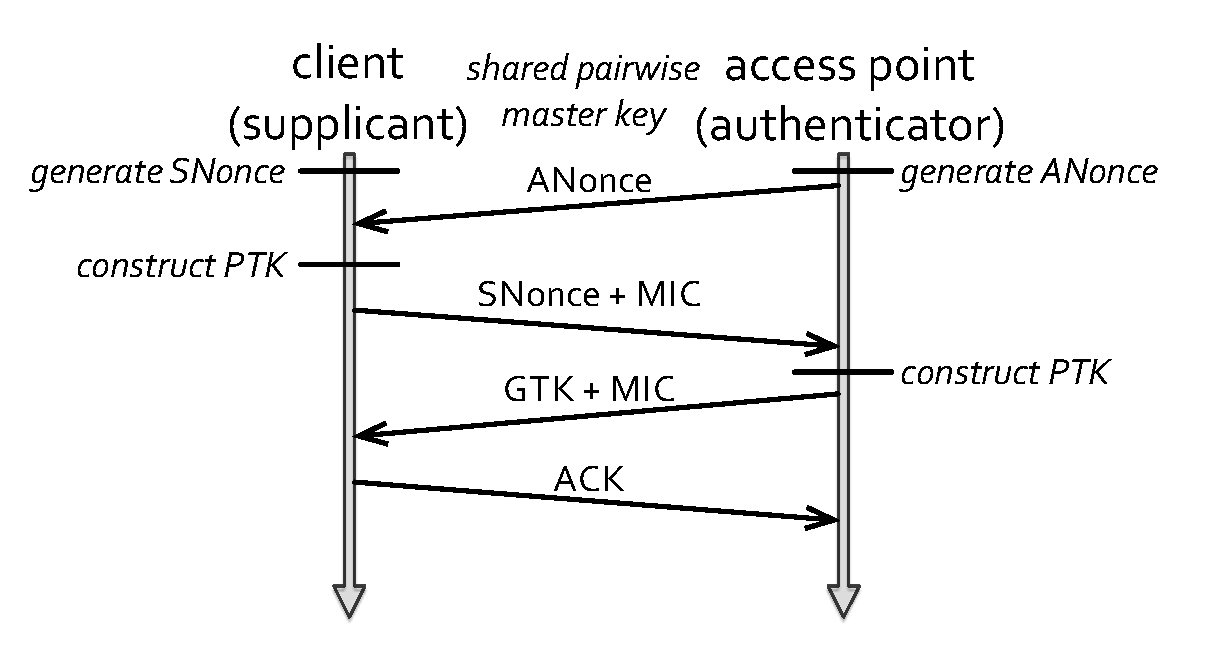
\includegraphics[width=0.8\columnwidth]{eapol}
  \caption{\label{f:association}802.11i handshake, part of the association
    process.  Note that MIC (Message Integrity Code) is an alternate term for
    MAC, used in such contexts to avoid confusion with Media Access Control.}
  \end{figure}
 
%% \mort{also intercept DNS- figures from previous section show that this
%%      will introduce negligible extra latency} 

Our home router supports wireless Ethernet security via 802.11i with EAP-WPA2,
depicted in Figure~\ref{f:association}, using \emph{hostapd}.  In EAP-WPA2
security mechanism, the
client (\emph{supplicant}) and our router (\emph{authenticator}) negotiate two
keys derived from the shared master key via a four-way handshake, through the
EAPOL protocol.  The \emph{Pairwise Transient Key} (PTK) is used to secure and
authenticate communication between the client and the router; the \emph{Group
  Transient Key} (GTK) is used by the router to broadcast/multicast traffic to
all associated clients, and by the clients to decrypt that traffic.  All
non-broadcast communication between clients must therefore pass via the router
at the link-layer (for decryption with the source's PTK and re-encryption with
the destination's PTK), although the IP routing layers are oblivious to this if
the two clients are on the same IP subnet.\footnote{The 802.11i specification
  defines a general procedure whereby two clients negotiate a key for mutual
  communication (\emph{Station-to-station Transient Key}, STK).  However, the
  only use of this procedure in the specification is in \emph{Direct Link Setup}
  (DLS) used in supporting 802.11e, quality-of-service.  This can easily be
  blocked by the access point, and in fact is not implemented in the
  \emph{hostapd} code we use, so we do not consider it further.
  %\mort{emphasise this bit?  also wifidirect - embedding of ``soft'' ap inside
  %wifi device - completely orthogonal?}i
  }

Periodically, a timeout event at the access point initiates rekeying of the PTK,
visible to clients only as a momentary drop in performance rather than the
interface itself going down.  We use this to apply blacklisting of clients
deemed malicious, such as a client that attempts to communicate directly (at the
link-layer) with another client, i.e.,~attempting to avoid their traffic being visible
to our home router.  We wait until the rekeying process begins and then decline
to install the appropriate rule to allow rekeying to complete for the client in
question.  This denies the client access even to link-layer connectivity, as
they will simply revert to performing the four-way handshake required to obtain
the PTK.  This gives rise to a clear trade-off between security and performance:
the shorter the rekeying interval, the quicker we can evict a malicious client
but the greater the performance impact on compliant clients.  

\begin{figure} \centering 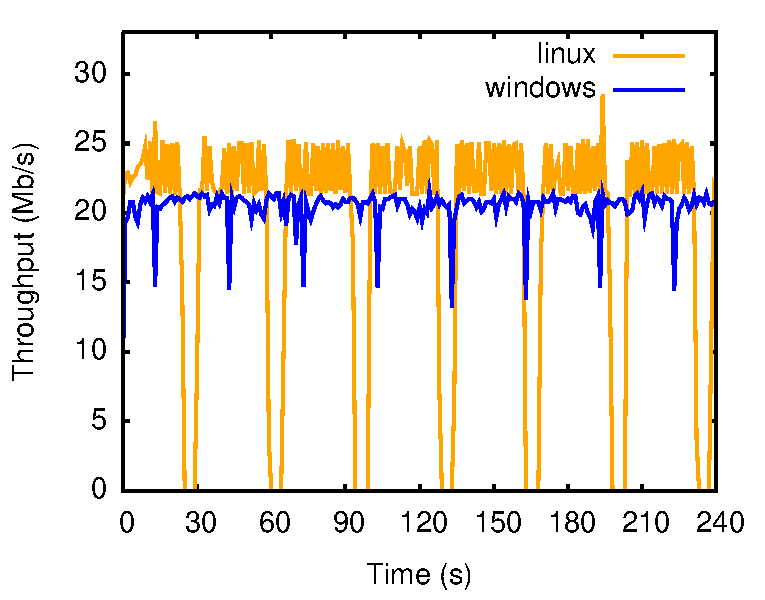
\includegraphics[width=0.7\columnwidth]{rekeying}
  \caption{\label{f:rekeying}Affect on TCP throughput from rekeying every 30s
    for Linux 2.6.35 using a Broadcom card with the \emph{athk9} module; and
    Windows 7 using a proprietary Intel driver and card.} 
\end{figure}

\begin{figure*} \centering
  % 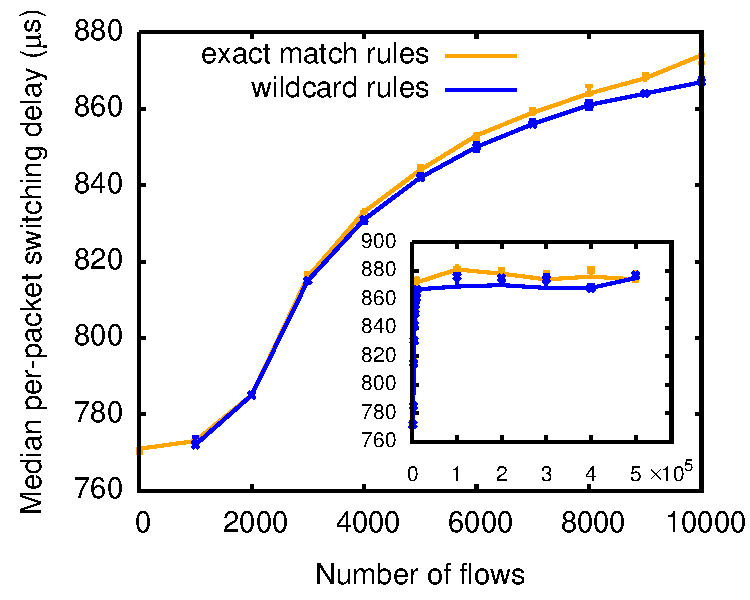
\includegraphics[width=0.49\columnwidth]{switching-delay}
  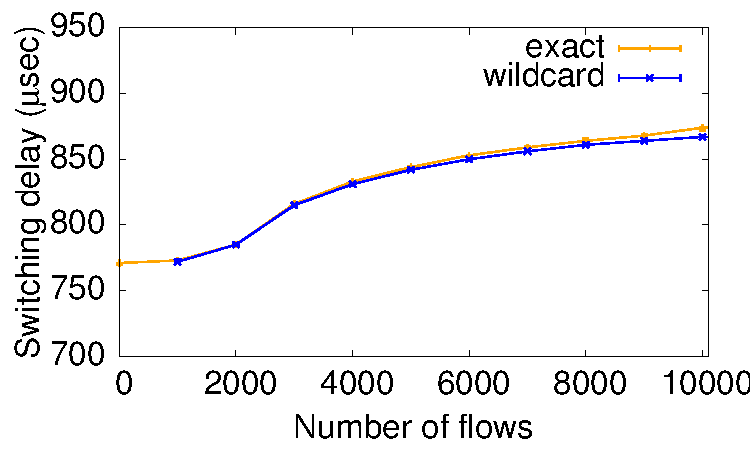
\includegraphics[width=0.49\columnwidth]{Chapter2/Chapter2Figs/latency-test}
%   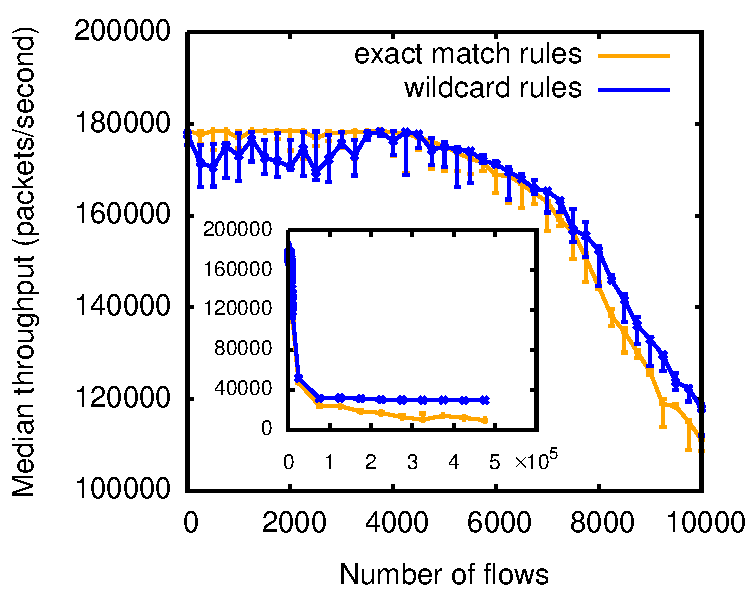
\includegraphics[width=0.49\columnwidth]{throughput}
   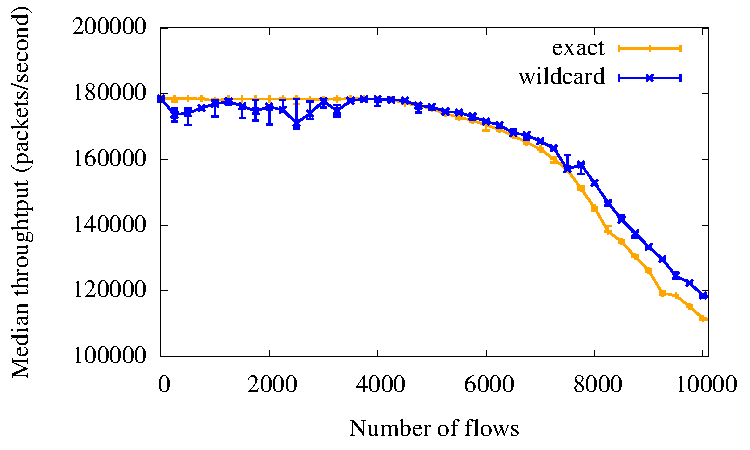
\includegraphics[width=0.49\columnwidth]{Chapter2/Chapter2Figs/throughput-test}
  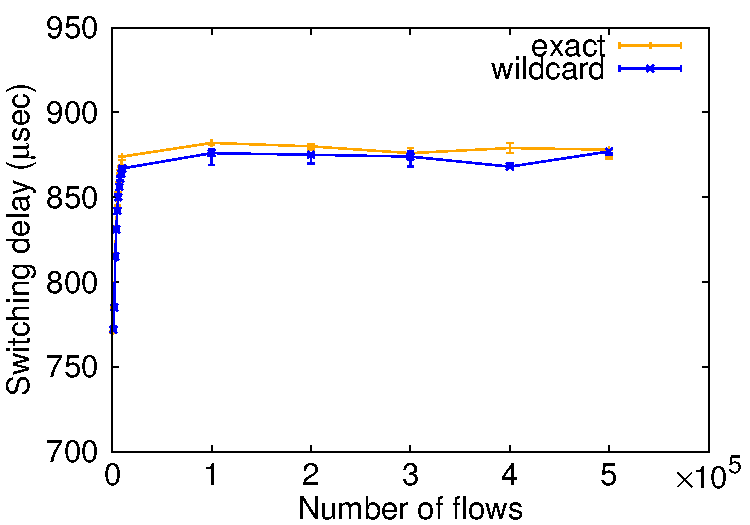
\includegraphics[width=0.49\columnwidth]{Chapter2/Chapter2Figs/latency-large-test}
   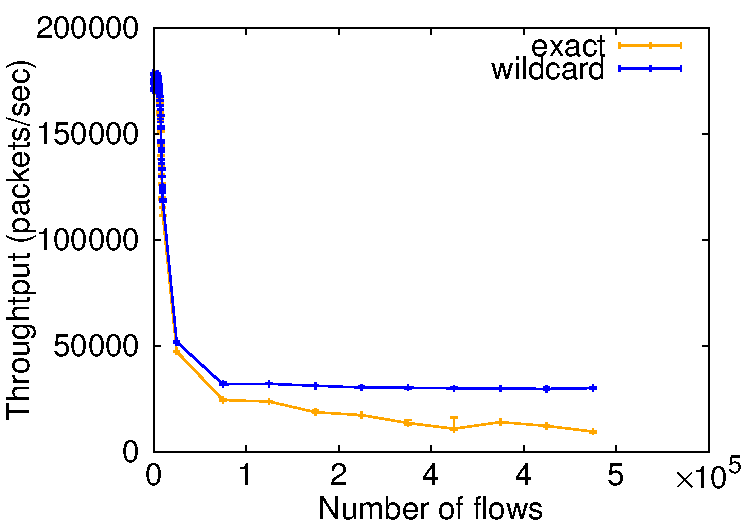
\includegraphics[width=0.49\columnwidth]{Chapter2/Chapter2Figs/throughput-large-test}
  \caption{\label{f:performance}Switching performance of \ovs component
    of our home router showing increasing per-packet latency (LHS) and
    decreasing packet throughput (RHS) with the number of flows.  The lower set
    of graphs extends the $x$-axis from 10,000 to 500,000.}
\end{figure*}

To quantify the impact of 802.11i rekeying, we observed throughput over several
rekeying intervals.  Figure~\ref{f:rekeying} shows the impact of setting the
rekeying interval to 30s: rekeying causes a periodic dip in throughput as the
wireless Ethernet transparently buffers packets during rekeying before
transmitting them as if nothing had happened.  This shows the trade-off between
performance and responsiveness of this approach: to be highly responsive in
detection of misbehaving clients imposes a small performance degradation.  As a
compromise, when a device is blacklisted, all of its traffic and subsequent
rekeying exchanges are blocked.  Thus the misbehaving device is prevented from
sending or directly receiving any traffic before rekeying takes place, The
device will be able to receive only broadcast traffic in the interim due, to the
use of the GTK for such frames, until the AP initiate the negotiation of a new
key.  This allows us to pick a relatively long rekey interval (5 minutes) while
still being able to respond quickly to misbehaving devices.

We also intercept DNS to give fine-grained control over access to Internet
services and websites.  DNS requests are intercepted and dropped if the
requesting device is not permitted to access that domain.  Any traffic the
router encounters that is not already permitted by an explicit OpenFlow flow
entry has a reverse lookup performed on its destination address.  If the
resulting name is from a domain that the source device is not permitted to
access, then a rule will be installed to drop related traffic.  Performance is
quite acceptable, as indicated by latency results in Figure~\ref{f:performance}:
the extra latency overhead introduced by our router is negligible compared to
the inherent latency of a lookup to a remote name server.  
% Extending this
% fine-grained control requires more accurate identification of traffic to
% application, particularly for more complex network uses such as BitTorrent and
% Skype, and is a problem we are investigating in ongoing work.

\subsection{Forwarding} \label{s:forwarding}
 
Our router consists of a single \ovs that manages interface
\emph{wlan0}.  \ovs is initialised with a set of flows that push
DHCP/BOOTP and IGMP traffic to the controller for processing.
\ovs by default will also forward to the controller traffic not matched
by any other installed flow, which is handled as follows:

\textbf{Non-IP traffic}.  The controller acts as a proxy ARP server, responding
to ARP requests from clients.  Misbehaving devices are blacklisted via a rule
that drops their EAPOL~\cite{rfc:3748} traffic thus preventing session keys
negotiation.
% implementing the WPA security association with the access point, so dropping
% it, prevents association.  
Finally, other non-IP non-broadcast traffic has source and destination MAC addresses verified
to ensure both are currently permitted.  If so, the packet is forwarded up the
stack if destined for the router, or to the destination otherwise.  In either
case, a suitable \of rule with a 30 second idle timeout is also installed to
shortcut future matching traffic.

\textbf{Unicast IP traffic}.  First, a unicast packet is dropped if it does not
pass all the following tests: 
\begin{itemize}
    \item its source MAC address is permitted; 
    \item its source IP address is in 10.2.x.y/16; and
    \item its source IP address matches that allocated by DHCP.  For valid
      traffic destined to the Internet, a flow is inserted that forwards packets
      upstream via the bridge and IP masquerading.  
\end{itemize} 
Unicast IP traffic that passes but is destined outside the home network has a
rule installed to forward it upstream via the bridge and IP masquerading.  For
traffic that is to remain within the home network a flow is installed to route
traffic as an IP router, i.e.~rewriting source and destination MAC addresses
appropriately.  All these rules are installed with 30s idle timeouts, ensuring
that they are garbage collected if the flow goes idle for over 30s.

\textbf{Broadcast and multicast IP traffic}.  Due to our address allocation
policy, broadcast and multicast IP traffic requires special attention.  Clients
send such traffic with the Ethernet broadcast bit\footnote{I.e.,~the most
  significant bit of the destination address} set, normally causing the hardware
to encrypt with the GTK rather than the PTK so all associated devices can
receive and decrypt those frames directly.  In our case, if the destination IP
address is all-hosts broadcast, i.e.,~255.255.255.255, the receiver will process
the packet as normal.  Similarly, if the destination IP address is an IP
multicast address, i.e.,~drawn from 224.*.*.*/4, any host subscribed to that
multicast group will receive and process the packet as normal. Finally, for
local subnet broadcast the router will rebroadcast the packet, rewriting the
destination IP address to 255.255.255.255. This action is required because the
network stack of the hosts filters broadcast packets from different IP subnets.

To assess switching performance, we examine both latency and packet throughput
as we increase the number of flows, $N$, from 1--500,000.  Each test runs for
two minutes, generating packets at line rate from a single source to $N$
destinations each in its own 10.2.*.*/30 subnet.  As these are stress tests we
use large packets (1500B) for the latency tests and minimal packets (70B)
\footnote{The 30B extra overhead is due to
  \emph{pktgen}~\cite{olsson05:_linux_packet_gener}, the traffic generation tool
  used.} for the throughput tests, selecting destinations at random on a
per-packet basis.  Results are presented as the median of 5 independent runs
with error bars giving the min and max values. 

Figure~\ref{f:performance} shows median per-packet switching delay and per-flow
packet throughput using either exact-match rules or a single wildcard rule per
host.  Performance is quite acceptable with a maximum switching delay of
560$\mu$s and minimum throughput of 40,000 packets/second; initial deployment
data suggests a working maximum of 3000 installed flows which would give around
160,000 packets/second throughput (small packets) and 500$\mu$s switching delay
(large packets).  Figure~\ref{f:stack-throughput} shows that the Linux
networking stack is quite capable of handling the unusual address allocation
pattern resulting from the allocation of each wireless-connected device to a
distinct subnet which requires the router's wireless interface to support an IP
address per connected device. Increasing the number of assigned IP address has
no impact on the processing latency and minimizes marginally the maximum packet
processing rate. This performance behaviour can also be explained by the trie 
data structure that the Linux kernel uses to lookup addresses; 
in the house setting the lookup takes O($log_2m$) time, where m is the
number of connected devices. 

\subsection{Discussion}

Our evaluation shows that \ovs can handle orders of magnitude more rules
than required by any reasonable home deployment.  Nonetheless, to protect
against possible denial-of-service attacks on the flow tables, whether
accidental or malicious, our home router monitors the number of
per-flow rules introduced for each host.  If this exceeds a threshold then
the host has its per-flow rules replaced with a single per-host rule, while the
router simultaneously invokes user interface callback to inform the homeowner of the
device's odd behaviour. 

The final aspect to our evaluation is compatibility: given that our router
exercises protocols in somewhat unorthodox ways, how compatible is it with
standard devices and other protocols?  We consider compatibility along three
separate dimensions: range of existing client devices; deployed protocols that
rely on broadcast/multicast behaviours; and support for IPv6. 

\begin{figure} 
  \centering 
  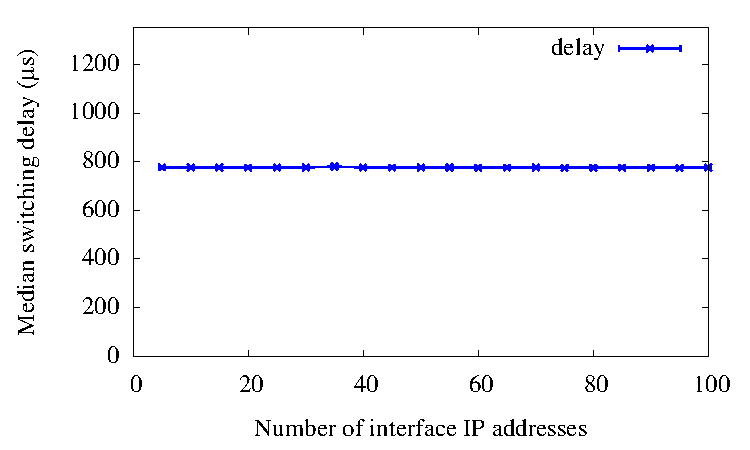
\includegraphics[width=0.49\columnwidth]{Chapter2/Chapter2Figs/stack-throughput-latency}
  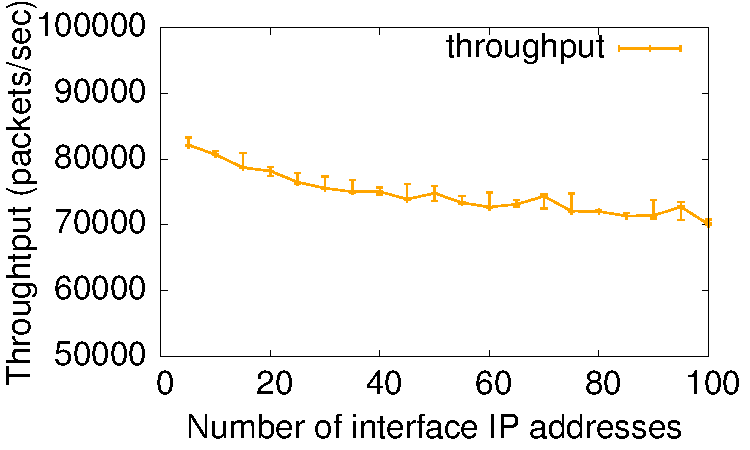
\includegraphics[width=0.49\columnwidth]{Chapter2/Chapter2Figs/stack-throughput-throughput}
  \caption{\label{f:stack-throughput}Switching performance of Linux network
    stack under our address allocation policy. Throughput (left figure) shows a
    small linear decrease while switching delay (right figure) remains
    approximately constant as the number of addresses allocated to the interface
    increases.} \end{figure}

\paragraph{Devices} Although we exercise DHCP, DNS and EAPOL in unorthodox ways
to control network access, behaviour follows the standards once a device is
permitted access.  To verify that our home router is indeed suitable for use in
the home, we tested against a range of commercial wireless devices running a
selection of operating systems. 

\begin{table*} \centering\footnotesize
  \begin{tabular}{lp{0.33\textwidth}p{0.42\textwidth}} \bf Device & \bf Denied &
    \bf Blacklisted\\

Android 2.x & Reports pages unavailable due to DNS.  & Retries several times
before backing off to the 3g data network.\\

iTouch/iPhone & Reports server not responding after delay based on configured
DNS resolver timeout.  & Requests new wireless password after 1--2 minutes.\\

OSX 10.6 & Reports page not found based on configured DNS resolver timeout.  &
Requests new wireless password after 1--2 minutes.\\

Microsoft Windows XP & Silently fails due to DNS failure.  & Silently
disconnects from network after 4--5 minutes.\\

Microsoft Windows 7 & Warns of partial connectivity.  & Silently disconnects
from network after 4--5 minutes.\\

Logitech Squeezebox & Reports unable to connect; allows server selection once
permitted.  & Flashes connection icon every minute as it attempts and fails to
reconnect.  \\ 

Nintendo Wii & Reports unable to reach server during ``test'' phase of
connection.  & Reports a network problem within 30s.\\

Nokia Symbian OS & Reports ``can't access gateway'' on web access.  & Reports
disconnected on first web access.\\ \end{tabular}
\caption{\label{t:devices}Observed interactions between devices and our home
  router when attempting to access the network.}
\end{table*}

Table~\ref{t:devices} shows the observed behaviour of a number of common
home-networked devices: in short, all devices operated as expected once
permitted access.  DNS interception was not explicitly tested since, as an
inherently unreliable protocol, all networking stacks must handle the case that
a lookup fails anyway.  Most devices behaved acceptably when denied access via
DHCP or EAPOL, although some user interface improvements could be made if the
device were aware of the registration process.  The social context of the home
network means no problem was serious: in practice the user requesting access
would be able to interact with the homeowner, enabling social negotiation to
override any user interface confusion. 

%% We initially investigated using different subnet allocations with
%% short (30s) lease times to more easily distinguish hosts that are
%% trying to connect but are waiting for the homeowner to permit them
%% access.  Unfortunately, due to a variety of issues with common client
%% DHCP implementations, e.g., Android not correctly obeying lease
%% times,\footnote{\url{http://www.net.princeton.edu/android/android-stops-renewing-lease-keeps-using-IP-address-11236.html}} 
%% this broke device interfaces sufficiently that doing so would only
%% increase user confusion.

\paragraph{Broadcast protocols} A widely deployed set of protocols relying on
broadcast and multicast behaviours are those for `zero conf' functionality.  The
most popular are Apple's \emph{Bonjour} protocol; \emph{Avahi}, a Linux variant
of Bonjour; Microsoft's \emph{SSDP} protocol, now adopted by the UPnP forum; and
Microsoft's \emph{NetBIOS}.  

Bonjour and Avahi both rely on periodic transmission of multicast DNS replies
advertising device capabilities via TXT records.  SSDP is similar, but built
around multicast HTTP requests and responses.  We tested Bonjour specifically by
setting up a Linux server using a Bonjour-enabled daemon to share files.  We
observed no problems with any clients discovering and accessing the server, so
we conclude that Bonjour, Avahi and SSDP would all function as expected. 

NetBIOS is somewhat different, using periodic network broadcasts to disseminate
hosts' capabilities.  In doing so we observed a known deficiency of NetBIOS: it
cannot propagate information for a given workgroup between different
subnets.\footnote{\url{http://technet.microsoft.com/en-gb/library/bb726989.aspx}}
However this was easy to overcome: simply install a WINS server on the router
and advertise it via DHCP to all hosts.
%\mort{although ugly, this would work at little cost and the other benefits seem
%significant. no extra attack surface because can configure nox/ovs/firewall to
%deny access to it from outside the home network}

In general, it may seem that our address allocation policy introduces link-layer
overhead by forcing all packets to be transmitted twice in sending them via the
router.  However this is not the case: due to use of 802.11i, unicast IP traffic
between two local hosts must \emph{already} be sent via the access point.  As
the source encrypts its frames with its PTK, the access point must decrypt and
re-encrypt these frames with the destination's PTK in order that the destination
can receive them.  Multicast and all-hosts broadcast IP traffic is sent using
the GTK, so can be received directly by all local hosts.  Only directed
broadcast IP traffic incurs overhead which though is a small proportion of the
total traffic; data from a limited initial deployment (about one month in two
homes) suggests that broadcast and multicast traffic combined accounts for less
that 0.1\% (packets and bytes) in both homes.
% \mort{cite?}
%, concurring with other larger (albeit non-domestic) datasets.  we have already
%discussed this previsouly : although other clients receive it at the
%link-layer, the address allocation policy means they will discard it, leaving
%it to the home router to replicate and retransmit all such traffic.  We do not
%consider this significant as data from a limited initial deployment (about one
%month in two homes) suggests that a very small amount of traffic is affected:
%broadcast and multicast traffic combined accounts for less that 0.1\% (packets
%and bytes) in both homes, concurring with other larger (albeit non-domestic)
%datasets.\mort{cite?}


\paragraph{IPv6 support} 

IPv6 support is once more receiving attention due to recent exhaustion of the
IPv4 address space.  Although our current implementation does not support IPv6
due to limitations in the current Open vSwitch and NOX releases,\footnote{\of
  provides support in its 1.4 release of the protocol; NOX currently has no
  support for IPv6; and \ovs only supports IPv6 as a vendor extension of the
  OpenFlow protocol.} we briefly discuss how IPv6 would be supported on our
platform.  While these limitations prevent a full working implementation in our
platform, we have verified that behaviour of both DHCPv6 and the required ICMPv6
messages was as expected, so we do not believe there are any inherent problems
in the approaches we describe below.

Addition of IPv6 support affects the network layer only, requiring consideration
of routing, translation between network and link layers, and address
allocation.  Deployment of IPv6 has minimal impact on routing, limited to the
need to support 128~bit addresses and removal, in many cases, of the need to
perform NAT.  \footnote{Some operators may still prefer to use NAT as part of a
  legacy of address management and operations.}  Similarly, supporting
translation to lower layer addresses equates to supporting ICMPv6 Neighbour
Solicitation messages which perform equivalent function to ARP.

%% During recent years a handful of ISPs started to provide IPv6
%% connectivity to clients and, since the exhaustion of IPv4 addresses
%% space, many more ISPs anounced their intetion to run production dual
%% stack networks. In order to address this trend as part of our design
%% we consider also an IPv6 scenario.  
%%                                     The addition of IPv6 support in
%% our design affects only the network layer of the protocol stack and
%% thus requires from us to reconsider three functionalities: routing, address
%% allocation and address translation to link layer. For the routing
%% process, the deployment of the IPv6 protocol has minimal impact to the
%% design (change of the length of the address) and in fact it reduces
%% complexity as it removes the nececity for NAT.

Address allocation is slightly more complex but still straightforward.  IPv6
provides two address allocation mechanisms: \emph{stateless} and
\emph{stateful}.  The first allows a host to negotiate directly with the router
using ICMPv6 Router Solicitation and Advertisement packets to obtain network
details, IP netmask and MAC address.  Unfortunately this process requires that
the router advertises a 64 bit netmask, of which current plans allocate only one
per household, with the result that all hosts would end up on the same subnet.
The second builds on DHCPv6 where addresses are allocated from a central entity
and may have arbitrary prefix length.  This would enable our router to function
in much the same manner as currently, although it would need to support the
ICMPv6 Router Advertisement message to support router discoverability by hosts. 

%% For the address allocation functionality, the introduction of the IPv6
%% protocol requires to change the functionality of the DHCP server. IPv6
%% provides 2 methods of address allocation in networks. The first
%% mechanism, called stateless address alocation, allows to a host to
%% self negotiate with the router, using ICMPv6 Router solicitation and
%% advertisment packets, the detail of the network and generate its IP
%% address using the subnet netmask and its MAC address.  Unfortunately,
%% this setup requires from the router to advertise a 64 bit long
%% netmask, resulting in all hosts being under the same network as,
%% according to current deployment plans, each ISP client is entitled to
%% a /64 prefix. The second mechanism, called stateful address
%% allocation, is build around the DHCPv6 protocol and is pretty similar
%% to the current DHCP mechanism implemented as part of our design. The
%% addresses are allocated from a central entity and can have arbitrary
%% prefix length. Additionally, since the DHCPv6 protocol doesn't aim to
%% configure routing for hosts, the router in required to implement
%% support for Router Advertsment message in order to allow hosts to
%% discover the router of the network.

%% Finally, in order to translate IPv6 addresses to lower layer
%% addresses, we need to enable on the router the ability to reply to
%% ICMPv6 Neighbour Solicitation message, similarly as in the case of ARP
%% packets.

%% While the implementation limitations noted above prevent a full
%% working implementation, we tested the basic functionality required by
%% our approach as follows.  

In order to test the functionality of our approach, we set up a simple hardcoded
version of our design. Specifically, we allocate a public IPv6 /64 prefix to our
home router. The router uses the ISC DHCPv6 server implementation, configured to
allocate addresses from a /120 subnet.  Additionally on the router we run the
RADVD daemon to reply appropriately to ICMPv6 messages.  Using this network
setup, we test MacOSX, Windows and Linux IPv6 network stacks and verified
correct network configuration and Internet connectivity. 


\section{User-centric resource allocation} \label{s:qos}

\begin{figure}
  \centering
  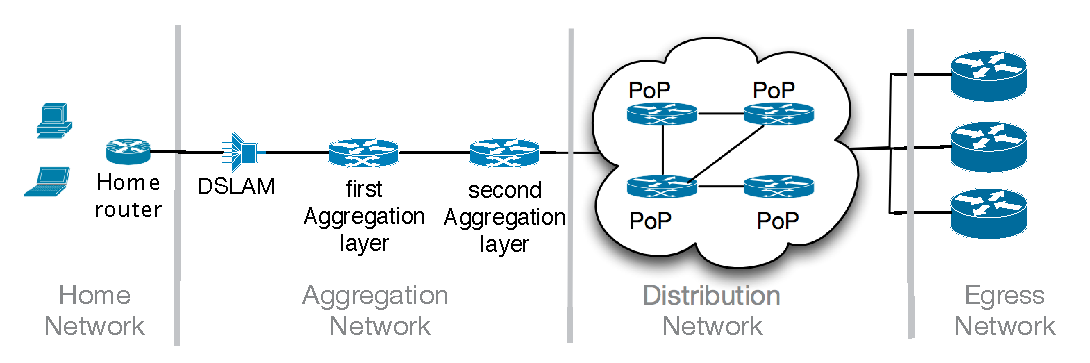
\includegraphics[width=0.95\columnwidth]{isp_plan}
  \caption{\label{fig:isp_plan} The path for each network packet of 
    the home network to the Internet. ISP network can be split in 3 parts:
  The {\it Aggregation Network}, the {\it Distribution Network}\/ and the {\it
    Egress Network}.}
\end{figure}

As we have discussed in Section~\ref{sec:intro:net_evolution}, network
application evolution has increased both the per-host resource requirements, as
well as, the complexity of the resource allocation mechanism. Effectively,
developing network architectures that can provide global application-specific
network performance guarantees is a difficult task. The network community uses
two common practices to tackle the resource allocation problem: network resource
over-provision and application-aware traffic engineering.  Resource
over-provision increases available resources, in order to remove performance
bottlenecks.  Application-aware network engineering extends the network policy
to  manage efficiently traffic from specific applications, e.g.~in an enterprise
network VoIP devices are connected to a separate high-priority VLAN\@. In
broadband networks these approaches have limited applicability. On one hand,
resource over-provision cost is non scalable on the edges of the broadband
network~\footnote{optical link installation cost varies between \$50-\$200 per
  foot, while fibers installation in municipal areas has an annual cost of
  \$1.91 per foot~\cite{backhaul-cost}. Upgrading such links also has a
  significant network equipment upgrade cost.}, while, on the other hand,
application-aware network engineering raises legal issues for Internet
providers~\cite{hahn06}. In this section, we propose an architectural extension
in the last-mile of the ISP, which enables homeowner to propagate
per-application resource requirements. Using this mechanism, we scale the
resource allocation problem in ISP management, while users can improve their
network experience and gain higher understanding .
In the rest of this section,  we present the architecture of current broadband
networks and discuss the inherent limitations in resource allocation
(Section~\ref{s:qos:motivation}), we present a highly efficient network
architecture for user-driven resource allocation
(Section~\ref{s:qos:architecture}) and evaluate the impact of our approach on
the performance of various traffic types (Section~\ref{s:qos:eval}).

\subsection{ISP resource allocation} \label{s:qos:motivation}

%This problem can be traced back
%to two main observations. Firstly, network performance has a multidimensional
%definition. Performance requirements may include limits over the  throughput and
%latency of a flow and are highly application-specific.  
%Secondly, home network traffic is highly asymmetric.
%Upload traffic volumes on average are significantly lower than download volumes.
%This is due, in part, to the properties of modern home network links, but also
%due to the nature of modern network applications that function in a
%client-server mode.  In order to control sufficiently resource allocation a
%system should consider independently both directions of the traffic. This is not
%thought possible for homeowners, as their network control is limited within the
%home network. 
% Download traffic, for example, is controlled by the
% home owner only on the last section of the path and thus we cannot develop a
% sufficient policy enforcing system that has traffic control solely within the
% home network limits.

In order to better introduce the reader to our system, we present in
Figure~\ref{fig:isp_plan} a visualisation of a broadband ISP network
architecture.  Although, exact network topology typically remains secret to each
ISP, there is a high level design pattern. In this figure we present the network
devices traversed by a packet sent from the home network to the Internet.  In
the Figure, we segment the network topology into four sections, the {\it home
  network}, {\it aggregation network}, {\it distribution network} and {\it
  egress network}. The aggregation network contains the Digital subscriber line
access multiplexer (DSLAM), translating DSL packets to Ethernet format over the
last mile,  the Broadband Remote Access Server (BRAS), an authenticating and
policy enforcing network device, and a number of layers of aggregation switches,
multiplexing the traffic from the various BRAS onto the distribution network.
Traffic from the aggregate network is routed through the distribution network
towards the egress network of the ISP or another aggregation switch, if the
packet is destined to an internal IP address. The distribution network consists
of a small number of large routers interconnected using high capacity links. An
ISP may typically use network tunnelling technologies, like MPLS, in the
distribution network, in order to reduce forwarding information on the routers.
The egress network of the ISP consist of large routers, hosted in AS IXP
networks and connecting the ISP with peering ASes and the rest of the Internet.

In the broadband network architecture, a number of research papers have
identified a significant bottleneck in the last-mile of the
network~\cite{Dischinger:2007bg,Akella2003}: the link between the DSLAM and the
aggregation network. This bottleneck can be explained by the high
oversubscription ratio of such links. The oversubscription ratio commonly varies
between the values 10:1 and 50:1~\cite{canada-subscription}, depending on the
number of users connected to the DSLAM, but it is not standardised and is
strongly affected by market dynamics~\cite{sky-oversubscription}.  

Through our network design, we aim to bridge a fundamental communication gap
between the ISP and homeowner. Users perceive network traffic as an ensemble of
flows belonging to a specific application; each application has a specific
prioritisation within the house context and the user-computer interaction,
e.g.~Skype VoIP traffic has a higher priority than web browsing traffic and
parents' teleworking traffic is more important than kids' entertainment traffic.
ISPs, on the other hand, manage the traffic of a specific household as a packet
aggregate with a specific source IP address and resource allocation mechanisms
are implemented as monthly or daily traffic caps for the specific IP
address~\cite{virgin-caps,bt-caps}.  Network caps  rate-limit heavy-hitting
households and provide long-term fairness between broadband users. Nonetheless,
this approach is not sufficient for a class of Internet applications, like
remote desktop and VoIP, for which performance is not tightly coupled with the
available bandwidth. Through our design, we believe that there is an incentive
for the ISP and homeowner entities to establish a
collaborative resource control framework. Homeowner can annotate high priority flows
within their traffic aggregate and thus improve user experience. ISPs can
increase user-friendliness of their network policy and offload some of the
complexity of their resource allocation mechanism to the end-users. 
% In addition, a sufficient
% resource mechanism requires the enforcement of the resource allocation policy
% both in the home network and within the ISP network. The bottleneck link of the
% network path is beyond the control of the homeowner and, since home traffic is
% highly asymmetric, the allocation policy cannot be implemented through control
% of a single traffic direction. 

Our architecture establishes a communication channel between the household and
the ISP and enables user-driven dynamically resource control on the bottleneck
link towards the aggregation network. More specifically, the ISP virtualises
switch resources over the last-mile and delegates control over a subset of the
available resources to a homeowner-managed \of controller.  In the virtualized
resources we additionally allocate minimum guaranteed bandwidth and a set of
hierarchical priority queues for each household. The household controller, in
real time, uses the \of protocol to forward high priority flows to the
appropriate priority queue. 

% Application priority policy  is
% express by the homeowner through a simple interface, that exposes application
% bandwidth consumption. 

While the proposed solution is not able to provide a complete system to
Internet-scale resource scheduling, we believe that it provides a sufficient
mechanism to handle in a user-friendly manner congestion on the edge-network and
scale the configuration complexity. 

% The
% architecture of the proposed system is described in Section~\ref{sec:qos_arch},
% while, in Section~\ref{sec:qos_eval}, we present a number of simple experiment
% to investigate the behaviour of the proposed system with various types of
% competing traffic.

\subsection{User - ISP communication} ~\label{s:qos:architecture}

In the proposed architecture we split system functionality between three
points in the network: a data-collection daemon on the end-systems of the home
network, a policy enforcing daemon on the home network router and an
\of controller to translate user performance requirements into ISP control
policy.

\paragraph*{End-system}

In order to map network flows to application, we develop a light cross-platform
daemon running on home network hosts and recording connection table content.
These information are collected from the connection table of the host network
stack and stored in the HWDB database. The daemon accesses the connection table
entries using the {\it netfilter-conntrack}~\cite{netfilter} in Linux systems,
the {\it Windows Filtering Platform}~\cite{win-wfp} in Windows systems and the
{\it sysctl} \/for Darwin/MacOSX system. 
% These libraries expose similar APIs and
% allow applications to register callbacks in the kernel network stack, which is
% triggered on every connection table change. 
In order to match each network tuple
with the respective applications, we use the {\tt lsof} command in unix-like
systems and the {\tt netstat -p} command in Windows.

\paragraph*{ISP infrastructure}

\begin{figure}
  \centering
  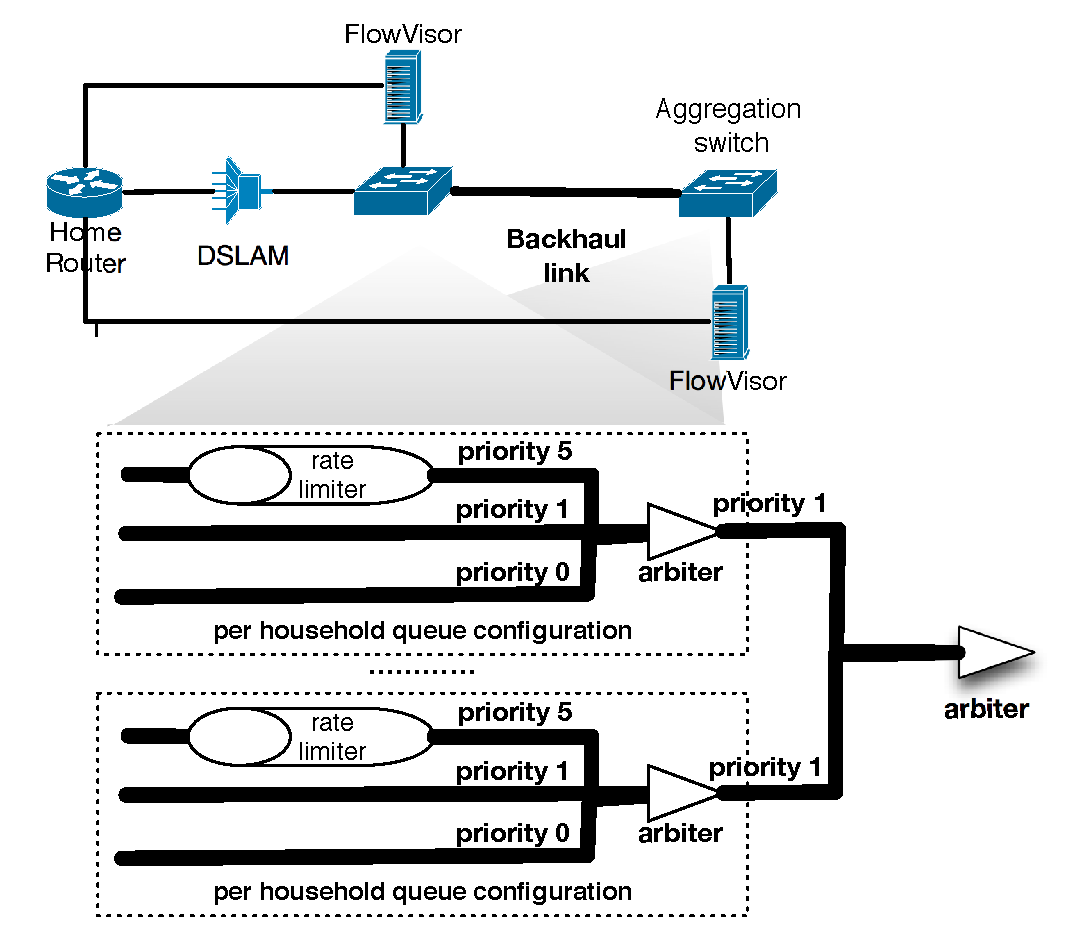
\includegraphics[width=0.7\columnwidth]{queue_design}
  \caption{User-driven network resource allocation architecture. 
    \label{fig:queue_design} Switch handling the downlink from the backhaul
    network exposes a
    virtual slice to the homeowner through a FlowVisor instance.  The switch
    allocates three queue primitives per-household: A {\it low latency,
      high priority} \/queue, a {\it medium priority} \/queue and a {\it default}
    \/queue.}
\end{figure}

We present the network on the edge of the ISP network in
Figure~\ref{fig:queue_design}.  In our user-centric resource allocation design
the first layer of aggregation switches must expose \of control.  The switch
control plane is virtualised using the FlowVisor
controller~\cite{flowvisor-osdi}. Each home router is running an \of controller
which connects to the FlowVisor service and exercises control over the home
Internet traffic. Specifically, the ISP virtualises the \of forwarding table and
exposes only a subset of the entries to each user.  The FlowVisor instance
propagates {\tt pkt\_in} messages to the home controller with a source or
destination IP address equal to the home public IP address and the FlowVisor
discards any {\it flow\_mod} packet which does not contain an equivalent IP
address. This FlowVisor configuration enforces a strong security mechanism; home
controllers cannot control or eavesdrop traffic from other households. 

At the aggregation switch and the home router we setup three priority queues for
each household (The home router queues handle the upstream traffic of the
household, while the aggregation switch queues handle the downstream traffic of
the household): A {\it low latency, high priority}~(LLHP) queue, a {\it medium
  priority}~(MP) queue and a default queue.  The LLHP queue has the highest
priority between the household queues and uses a leaky bucket mechanism to rate
limit traffic to the minimum guaranteed bandwidth per-household. This queue can
be used by low-bandwidth low-latency applications. The HP queue doesn't enforce
any rate limit, but it has a priority which is between the LLHP and the default
queue.  HP queue can be used by latency-tolerant high-priority applications.
Finally, the default queue is used to handle all other traffic types.  The queue
hierarchies from each household are multiplexed towards the output port with
equal priorities.  Large scale queue hierarchies are currently supported by
service provider grade network equipment (e.g.~Cisco ASR 9000 router provide
500k queues per line card~\cite{cisco-asr-qos}) and ISPs use this functionality
to implement their capping policy. By default, all network flows are forwarded
to the default queue and the home \of controller at run-time can assign flows to
higher priority queues based on the user configured policy.  This resource
allocation mechanism is constraint per-household by the number of flows that the
FlowVisor exposes to each home.  This network design can be extended to evolve
further the ISP broadband economical model; Users can enhance network
performance by purchasing additional flow table entries and increase minimum
guaranteed bandwidth on the edge. 

Because our system design provides extensive forwarding control to end-users, we
fortify the design with a set of mechanisms to reduce the ability of end-users
to compromise network functionality.  Firstly, fair allocation of flow table
entries to each household, ensures fair utilisation of the forwarding resources
in the aggregate switch. Secondly, the FlowVisor instance rate limits \of
control channel interactions per household to mitigate DoS attacks. Finally, the
Flowvisor instance discards flows that may create loops in the network,
e.g.~{\tt flow\_mod} messages with an Output action  that forwards packet to the
incoming port. 

\paragraph*{Home Router}

\begin{figure}
  \centering
  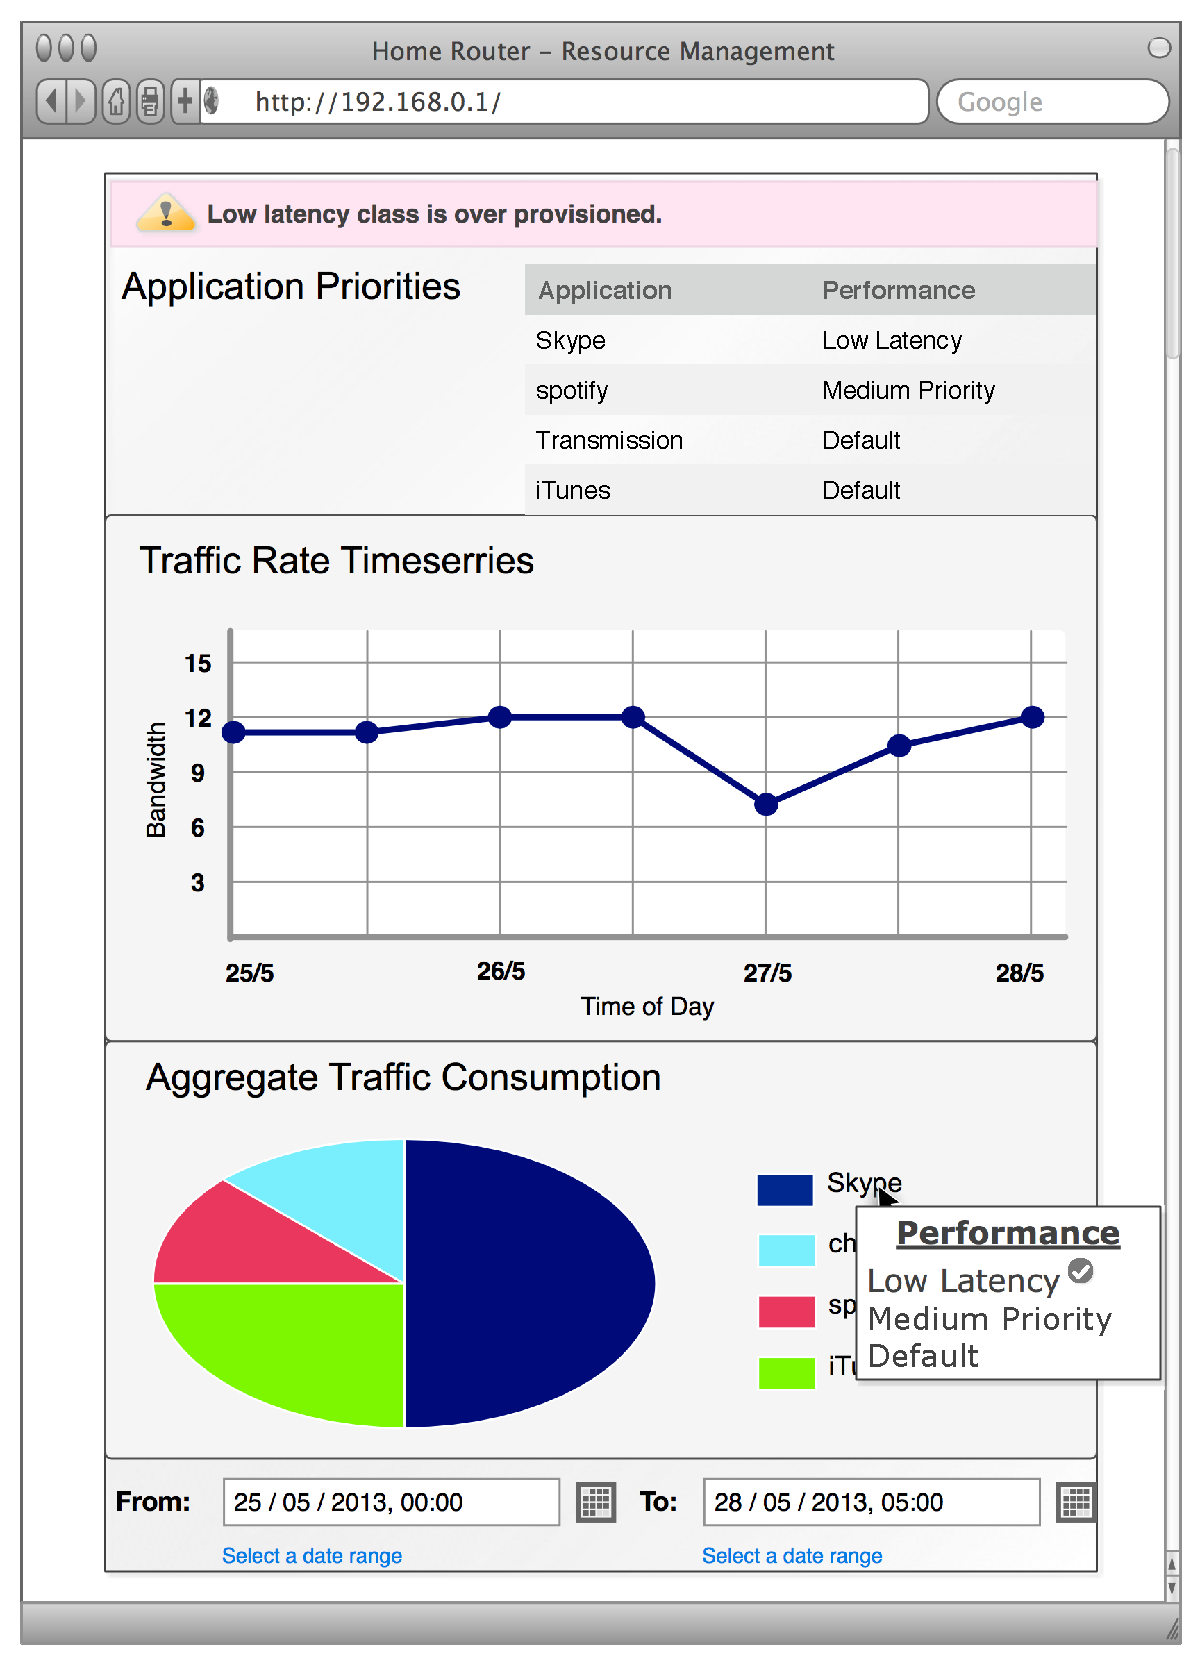
\includegraphics[width=0.8\columnwidth]{homework_intf_qos}
  \caption{\label{fig:homework_intf_qos} Performance mechanism  user control.
    The user is able to view the network utilisation per application, as well as
    express application prioritisation.}
\end{figure}

In our design, the home router is the rendez-vous point between the
policies of the two network. In order to support the state requirements of this
functionality we add in the hwdb database three new tables: {\it Application
  tuple}, {\it Application timeseries} and {\it Application priorities}.
Application tuple table stores mappings between applications and 
network tuples. This table is populated with data from the end-hosts, while the
router installs a monitoring hook in order to receive new flow arrivals.
Application timeserries table stores per-application network utilization
information. The table is populated with data from the router using the
flow stats message of the \of protocol, while the data are used by the web
visualisation in order to inform users for the per-application network consumption. 
Finally, the Application priority table stores theapplication prioritisation
policy pf the user. This table is populated with data through the interface
of the system and the controller uses it to map new flows to the appropriate
queue.

We expose the resource management mechanism through a user-friendly web
interface depicted in Figure~\ref{fig:homework_intf_qos}.  Through this
interface the user can view the aggregate and time serries resource consumption
per application and configure application priority policy. Additionally, the
interface notifies the user when the policy over-utilizes the LLHP queue.
Specifically, we use the packet loss counter of the \of {\tt queue\_stats}
message to trigger notifications during high packet loss incidents.  Through
this interface we try to address the issues raised by the work
in~\cite{Chetty10}. 

During operation, the proposed design extends the forwarding logic described
earlier. Specifically, for each network flow, once the controller has verified
that the flow is in accordance with the policy and destined to a non-local IP
address, the controller maps the flow to an application and to a priority queue,
through the HWDB database. The controller sends a {\tt flow\_mod} message with an
{\tt enqueue} action to assign the flow to the appropriate queue. In addition,
if the application priority is not the default, then the controller will also
send a {\tt flow\_mod} packet to the FlowVisor instance, to setup the incoming
direction of the flow. 
% In order to ensure that there is an
% application mapping for the flow, in case of an incoming connection the switch
% will establish only the incoming direction if the flow on the local switch and
% will assign queue only when the outgoing direction of the flow is used. This way
% we will have ensured that the end-host daemon will have inserted the appropriate
% information. 

\subsection{Evaluation} \label{s:qos:eval}

\begin{figure}
  \centering
  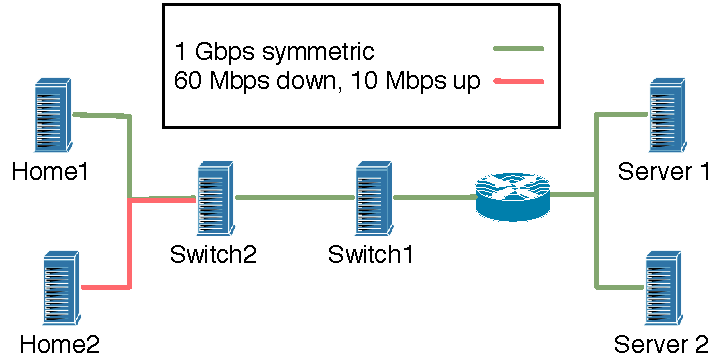
\includegraphics[width=0.8\columnwidth]{queue_eval_setup}
  \caption{\label{fig:queue_eval_setup} Experimental setup to evaluate the
    proposed resource management system.}
\end{figure}

We evaluate the proposed architecture using a lab testbed, depicted in
Figure~\ref{fig:queue_eval_setup}. {\it Home1} and {\it Home2} emulate the
networking activity of an ensemble of Home Connections. We focus the
analysis on the behaviour of Home2, that emulates a single connection in the
vicinity of an ensemble of Home connections, emulated by node Home1. 
{\it Server1} and {\it Server2} instances run a number of listening daemon that
generate traffic, based on traffic requests, from the Home instances and
simulates Internet wide Services. Fιnally, {\it Switch1} and {\it  Switch2}
emulate the switches that control the backhaul link. Steady state TCP is
generated using the iperf tool~\cite{iperf}. We also utilize pttcp tool, in
order to simulate stochastic models of short lived TCP flows. 

\section{Conclusions} \label{s:conclusion}

This paper has drawn upon previous user studies to reflect on the distinctive
nature of home networks and the implications for domestic network
infrastructures.  Two particular user needs that arose from these studies were
for richer visibility into and greater control over the home wireless network,
as part of the everyday management of the home by inhabitants.  We  considered
how to exploit the nature of the home network to shape how it is presented and
opened to user control.  

Simply put, the home is different to standard networking environments, and
many of the presumptions made in such networks do not hold.  Specifically,
home networks are smaller in size, the equipment is physically accessible and
access is often shared among inhabitants, and the policies involved are
flexible and often dynamically negotiated.  Exploiting this understanding
allows us to move away from traditional views of network infrastructure, which
must be tolerant of scale, physically distributed, and impose their policies
on users. 

We use the \ovs and NOX platforms to provide flow-based management of
the home network.  As part of this flow-based management, we exploit the
social conventions in the home to manage introduction of devices  to the
network, and their subsequent access to each other and Internet hosted
services.  This required modification of three standard protocols, DHCP, EAPOL
and DNS, albeit in their behaviour only \emph{not} their wire formats, due to
the need to retain compatibility with legacy deployed stacks.
                                                         
Our exploration suggests that, just as with other edge networks, existing
presumptions could usefully be re-examined to see if they still apply in this
context.  \emph{Do we wish to maintain net neutrality in the home?}
Inhabitants do not appear to see network traffic as equal, often desiring
imbalance in performance received by different forms of traffic.  \emph{Must
the end-to-end argument apply?} Householders understand and exploit the
physical nature of their home and use trust boundaries to manage access; we
have exploited these resources to explicitly manage the network.  \emph{Should
communication infrastructures remain separate from the devices that use them?}
In the home setting this separation proves problematic as people, ranging from
the home tinkerer to the DIY expert, wish to interact directly with the
network as they do with other parts of their homes' physical infrastructures.
Our exploration suggests use of a range of displays and devices existing not
as clients exploiting the infrastructure but as extensions of the
infrastructure making it more available and controllable.

Inability to understand and control network infrastructure has made it
difficult for people to understand and live with it in their homes.  We have
developed a home router that both captures information about people's use of
the network and provides a point of interaction to control the network.  Our
initial developments have explored the extent to which residents may be
involved in some of the protocols controlling the network; other protocols
suitable for modification are under consideration.

%\section{Related Work} \label{s:related}
% 
%Many authors have argued that home networks should be treated differently to
%other IP-based networks.  For example, Calvert
%\etal.~\cite{calvert07:_movin_towar_middl} make a case against application of
%the end-to-end principle in home networking.  They argue that there are a
%number of key aspects peculiar to the home environment that the standard
%Internet protocols do not address.  They derive a series of requirements for a
%home network architecture, and a design providing functions to fulfil these
%requirements.  Many of the points they make, e.g., their ``smart middle''
%design, resonate with our argument, and indeed, we believe our home router
%meets the requirements and provides the functions they describe.
%
%%% \mort{no need to spend so much on interfaces- a sweeping ``but they
%%%  don't go deep enough to be interesting'' should be enough}
%Both before and after the general architectural arguments made above, a number
%of authors have proposed novel user interfaces to aid the homeowner in managing
%their network.  GesturePen~\cite{swindells02:_that} uses line-of-sight radio
%interaction with purpose-built receiver tags to control network access;
%Network-in-a-Box~\cite{balfanz04:_networ}, where infrared port alignment
%provides a physical metaphor for access, plugging in to security mechanisms
%such as EAP-TLS and RADIUS.  They also describe an interesting ``phone home''
%service via the Windows Remote Access and IPSec policy mechanisms that enables
%remote clients to connect back to appear as if inside the home network.
%
%ICEBox~\cite{yang07:_icebox} again concentrates on the problem of enabling the
%homeowner to correctly configure new devices when they are brought onto the
%network using a control panel approach similar to our Guest Board.  They note
%that a future version might well subsume the home router.
%Eden~\cite{yang10:_eden}, by several of the same authors, follows this up by
%replacing the home router.  Their implementation allows per-flow traffic
%control, but the paper lacks technical details.
%%   makes use of the standard Linux \emph{tc} and
%% \emph{iptables} facilities to allow the homeowner to exercise per-flow
%% traffic control; they do not discuss technical specifics in any
%% detail.
%
%All these approaches primarily address the interaction design problem, focusing
%on user interface solutions to the problems of managing a home network.  Most
%rely upon specialized hardware or software installation on client devices.  In
%contrast, our home router does not require client modification as its protocol
%modifications are fully backward compatible with existing stacks.  It thus
%supports a very wide range of devices while making possible greater control of
%connectivity.
%
%%% \mort{probably need to leave following refs in}
%
%% Addressing the problems of troubleshooting,
%% Netprints~\cite{aggarwal09:_netpr} is a system for cooperative
%% diagnosis of home network misconfigurations.  They take a black-box
%% approach in that they do not predefine specific models, and they focus
%% on application specific problems rather than the home network as a
%% whole.  Client software scrapes labeled configuration information from
%% devices, and computed feature vectors describing the more dynamic
%% aspects of the system (e.g., observed traffic).  These data are
%% collected in a central server and fed into a decision tree based
%% learning system to perform subsequent diagnoses given observed data.,
%% Kandula \etal.~\cite{kandula09:_detail} also proposed a system for
%% diagnosis of problems, aimed specifically at small enterprise
%% networks.
%
%Several authors have proposed solutions to the specific problem of lack of
%visibility into what the network and connected devices are doing.  In this
%context, HostView~\cite{joumblatt10:_hostv} uses a client daemon to log when
%users experience network problems.
%% also relies on client
%% software but focuses more simply on generating labeled data by
%% enabling the user to notify the system when some user-perceived
%% problem occurred.  
%Calvert \etal.~\cite{calvert10:_instr_home_networ} present requirements for a
%general purpose ``always on'' local logging service, building a simple example
%using \emph{tcpdump} running on a
%NOXBox,\footnote{\url{http://www.noxrepo.org/manual/noxbox.html}} dumping
%traffic into flat files.  Both focus on network monitoring as a tool for
%troubleshooting.  Finally, in presenting the Homework Database, Sventek
%\etal.~\cite{sventek11:_infor_plane_archit_suppor_home_networ_manag} describe
%it as a component in their home network information plane.  Their system uses a
%general-purpose policy engine to exercise control over the network by
%configuration of the router derived from the interaction of monitored data and
%policy.
%
%We claim that, in general, these monitoring systems do not take into account
%the specific challenges and opportunities inherent in the home network context.
%Our home router goes further in exploiting the home context via specific
%modifications to the normal behaviour of key protocols, as well as implementing
%a novel network control interface.
%
%This class of argument, that the generic Internet protocols are not appropriate
%in a particular environment, has previously been made in the enterprise network
%space.  Approaches such as Anemone~\cite{cooke06:_reclaim},
%Ethane~\cite{casado07:_ethan} and Network Exception
%Handlers~\cite{karagiannis08:_networ} have all proposed systems that address
%the general problem of enterprise network management in different ways.  They
%all make the argument that enterprise networks are basically different to the
%traditional Internet, presenting different problems and permitting different
%solutions.  This resonates strongly with our claims that home networks should
%be treated differently, and in some ways with our approach of providing more
%intelligent centralised control.  It should be noted however, that these
%enterprise network solutions are no more applicable to home networks than
%traditional Internet approaches were applicable in the enterprise!
%
%Finally, looking back to 1984 and some of the original discussions of IP
%subnetting, Mogul~\cite{rfc:917} and Postel~\cite{rfc:925} discussed using
%subnetting to hide site LAN interconnection from networks outside the site.
%They introduce techniques such as ARP-based subnetting, ARP bridging, and
%extension of ARP itself.  ARP bridging in particular is very similar in
%practice to the approach we take, although we assign a subnet per-host rather
%than per-LAN, and we manage address allocation and connectivity using protocols
%unavailable at the time.

%% \mort{add intserv, maybe diffserv refs - note different domain and
%%  scale} 

% \section{Conclusions} \label{s:concl}
%  
% This paper has drawn upon previous user studies to reflect on the distinctive
% nature of home networks and the implications for domestic network
% infrastructures.  Two particular user needs that arose from these studies were
% for richer visibility into and greater control over the home wireless network,
% as part of the everyday management of the home by inhabitants.  We  considered
% how to exploit the nature of the home network to shape how it is presented and
% opened to user control.  
% 
% Simply put, the home is different to standard networking environments, and
% many of the presumptions made in such networks do not hold.  Specifically,
% home networks are smaller in size, the equipment is physically accessible and
% access is often shared among inhabitants, and the policies involved are
% flexible and often dynamically negotiated.  Exploiting this understanding
% allows us to move away from traditional views of network infrastructure, which
% must be tolerant of scale, physically distributed, and impose their policies
% on users. 
% 
% We use the \ovs and NOX platforms to provide flow-based management of
% the home network.  As part of this flow-based management, we exploit the
% social conventions in the home to manage introduction of devices  to the
% network, and their subsequent access to each other and Internet hosted
% services.  This required modification of three standard protocols, DHCP, EAPOL
% and DNS, albeit in their behaviour only \emph{not} their wire formats, due to
% the need to retain compatibility with legacy deployed stacks.
%                                                          
% %%                                                          platofrm
%                           
% %% We draw upon these characteristics of the network and the social %%
% conventions of the home to develop two distinct mechanisms, %% implemented
% using the NOX and \ovs platforms as part of a %% redevelopment of the
% home router.  The first exploits the social %% conventions of visiting to
% manage the introduction of machines to the %% network.  This is reflected in a
% modification to the DHCP protocol to %% put people explicitly inside the
% protocol, allowing the homeowner to %% be prompted for advice and information.
% The second exploits the home's %% physical arrangement to develop a physical
% approach to access control %% based on commodity USB storage keys.  
% 
% Our exploration suggests that, just as with other edge networks, existing
% presumptions could usefully be re-examined to see if they still apply in this
% context.  \emph{Do we wish to maintain net neutrality in the home?}
% Inhabitants do not appear to see network traffic as equal, often desiring
% imbalance in performance received by different forms of traffic.  \emph{Must
% the end-to-end argument apply?} Householders understand and exploit the
% physical nature of their home and use trust boundaries to manage access; we
% have exploited these resources to explicitly manage the network.  \emph{Should
% communication infrastructures remain separate from the devices that use them?}
% In the home setting this separation proves problematic as people, ranging from
% the home tinkerer to the DIY expert, wish to interact directly with the
% network as they do with other parts of their homes' physical infrastructures.
% Our exploration suggests use of a range of displays and devices existing not
% as clients exploiting the infrastructure but as extensions of the
% infrastructure making it more available and controllable.
% 
% Inability to understand and control network infrastructure has made it
% difficult for people to understand and live with it in their homes.  We have
% developed a home router that both captures information about people's use of
% the network and provides a point of interaction to control the network.  Our
% initial developments have explored the extent to which residents may be
% involved in some of the protocols controlling the network; other protocols
% suitable for modification are under consideration.  We are currently involved
% in the deployment and study of use of our home router to better understand
% relevant user needs and how we might more systematically exploit the data we
% are collecting.  We are also exploring how to use this data in other areas
% such as security and power management.  


%%% Local Variables: 
%%% mode: latex
%%% TeX-master: "../thesis"
%%% End: 

\chapter{Secure and Scalable Internet-scale Connectivity}
\label{sec:signpost}
\ifpdf
    \graphicspath{{Chapter3/Chapter3Figs/PNG/}{Chapter3/Chapter3Figs/PDF/}{Chapter3/Chapter3Figs/}}
\else
   \graphicspath{{Chapter3/Chapter3Figs/EPS/}{Chapter3/Chapter3Figs/}}
\fi

In this chapter we explore application of the SDN technology in connectivity and
naming scalability.  The work is motivated by the user requirement to create a
network federation between its devices.  We call this functionality a
\emph{Personal Cloud}.  Currently, Personal Clouds use third-party Cloud
services as information caches, to bridge the inter-device communication
requirements. Device federation is currently limited due to the connectivity and
naming limitations of the Internet architecture.  This architecture is a
consequence of the connectivity scalability limitations of the Internet, as
discussed in Section~\ref{sec:intro:motivations}. Nonetheless, as users offload
personal information to third-party services, they become subject to privacy
threats and performance degradation.

We argue that end-devices require an adaptable network control architecture, in
order to overcome  connectivity limitations and control their data and
resources.  The network community provides an abundant of free and open
mechanisms, which can be reused dynamically to provide inter-device
connectivity.  We introduce \signpost, a network control plane for end-devices,
capable of delivering continuous and secure connectivity between user devices.
\signpost integrates existing network testing approaches to detect network
environment conditions and configures existing software packages to establish
end-to-end connectivity between devices. 

In order to understand the feasibility and performance of the proposed
architecture, we present a strawman implementation of the core control logic and
its integration with a number of network connection and notification services.
Currently, \signpost supports SSH~\mycite{RFC4245}, OpenVPN~\mycite{openvpn},
TOR~\mycite{dingledine2006}, NAT-punch and Privoxy~\mycite{privoxy} 
mechanisms, while it can also propagate Multicast-DNS notifications across
devices.

For the rest of this chapter, we present a preliminary categorisation of
Personal Cloud platforms and, motivated by some key observation, we define the
key design requirements for our
platform~(Section~\ref{sec:signpost-introduction}). Furthermore, we present the
\signpost abstraction~(Section~\ref{sec:sp-signpost}) and
architecture~(Section~\ref{sec:signpost-architecture}), followed by an elaborate
description of a strawman \signpost implementation and an evaluation of its
functionality~(Section~\ref{sec:signpost-evaluation}).  Finally, we conclude our
observations~(Section~\ref{sec:signpost-conclusion}).

\section{Personal Clouds}\label{sec:signpost-introduction}

The digital revolution of our era has mirrored a large part of our life in the
digital domain. For example, human labour is commonly stored in PDF and word
processing files, while social interactions are partially captured in digital
photo collections.  Effectively, our physical presence has an increasing digital
counterpart, accessible primarily through computing devices.  Nonetheless, the
increase in the adoption of personal computers introduces challenges in the
management of our digital footprint.  Complimentary to personal computers, users
currently own and use tablets, smartphones and other purpose-build computing
units (e.g.~home entertainment systems and gaming consoles), while the IoT
paradigm~\mycite{Atzori2010} will extend further.  From a user perspective, each
device fulfils a specific role in managing digital resources, thus requiring
access only to a subset of the user digital presence, but these roles are fluid
and intercept.  For example, a smartphone is primarily a communication device,
but end-users may use it as a media player. In the latter case, the smartphone
and the home entertainment system provide similar functionality to the user and
require access to the same subset of his digital presence. As a result, the
transition from a single PC to a multi-device paradigm requires global and
homogeneous access and control mechanisms of digital information and
resources. We define this abstraction as the user \emph{Personal Cloud}. 

This section presents existing Personal Cloud mechanism and discusses their
functional limitations~(Section~\ref{sec:sp-approaches}) and defines the core
\signpost design goals~(Section~\ref{sec:sp-challenges}). 

\subsection{Approaches} \label{sec:sp-approaches}

Personal Cloud functionality is readily available in a number of applications,
providing a wide range of abstractions. This section provides a simple taxonomy,
based on their architecture. 

\paragraph*{Decentralised Personal Cloud}

Decentralised Personal Cloud application class contains standalone
connectivity mechanisms, managed by end-users.  Computer networks by design 
provide the middleware to enable information and resources sharing between
computers. As a result, the network community provides an extensive collection
of applications and protocols supporting Personal Cloud functionality, such as
remote desktop access (e.g.~Remote Frame Buffer protocol~\mycite{RFC6143}), file
sharing (e.g.~NFS~\mycite{RFC1094}, SAMBA file service~\mycite{samba}), remote login
(e.g.~SSH~\mycite{RFC4253}), remote printing (e.g.~IPP~\mycite{RFC2911})~et al.
Such systems employ a client-server architecture and extend the computer
abstraction to preclude inter-device connectivity.  A user can setup and manage
sharing services on his personal devices and enhance his computing experience.
Furthermore, the setup complexity of some services has motivated the
development of automation mechanisms like Multicast-DNS, UPnP and ZeroConf,
which allow a user to seamlessly browse and access available services. 

Decentralised Personal Cloud applications provide extensive control over
personal data and strong privacy guarantees. Decentralised approaches are a
popular mechanism to share data  within the local network, like the home
network, Nonetheless, Internet-scale deployment of such mechanism faces
significant scalability problems, primarily due to the following three issues:

\begin{itemize}
  \item {\it Connectivity}\/: Decentralised Personal Cloud effectiveness is
    defined by Internet connectivity limitations.  The current Internet
    architecture does not guarantee global and homogeneous service
    accessibility, as we have discussed in Section~\ref{sec:intro:motivations},
    limiting the applicability of client-server models.  End-users commonly
    connect to the Internet through edge networks optimised for outgoing
    connectivity, while ubiquitous middleboxes limit service accessibility. For
    example, NATed networks by default restrict incoming Internet connectivity,
    while mobile and enterprise networks enforce network policies, using
    firewalls, which limit device connectivity for security reasons.

  \item {\it Authentication}\/: In the context of security, there are two  
    primary authentication architectural paradigms: out-of-band communication
    and pre-deployed information~\mycite{RFC5387}. The majority of decentralised
    applications use pre-deployed authentication mechanisms, based either on
    password or public key schemes. Although the approach is effective, it
    exhibits limited flexibility to support management automation and
    responsiveness to user credentail compromises. Out-of-band
    authentication mechanisms address effectively the aforementioned problems,
    but existing applications often lack support, while enabling such mechanism
    requires significant management effort. 

  \item {\it Usability}\/: Decentralised Personal Cloud applications introduce
    significant usability challenges to inexperienced users. Configuration
    interfaces of relevant software vary significantly, while in some cases
    effective configuration requires deep understanding of the system (e.g.~the
    SSH client in Linux has 26 command line parameters and 70 configuration
    options).  In addition, due to the previously discussed connectivity
    limitations, users must resolve to a ``trial and error'' approach to
    evaluate the effectiveness of an application configuration in a specific
    environment and potentially use multiple mechanisms to achieve
    connectivity, like tunnelling software.  Effectively, the configuration of
    decentralised personal cloud applications is complex and long in terms of
    time,  highly disengaging for inexperienced users, as discussed in
    Section~\ref{s:evolution}.\\ 
    As an example, we describe the required steps to access files from a remote
    device using the SSH service, following the decentralised approach. Initially,
    the user must configure the SSH service on the server host, both in terms of
    access control and service functionality, and any firewall and NAT device
    deployed in the local network. Additionally, the user must configure
    dynamically a naming service if the public IP of the server is dynamic,
    e.g.~DynDNS~\footnote{\url{http://dyn.com/dns/}}\@.  SSH connectivity is
    subject to the ability of the user in the remote network to use the SSH
    protocol on the preconfigured port.  In case this is not possible, the
    user has to try a different connection establishing mechanism.
\end{itemize}

\paragraph*{Centralised Personal Cloud}

A popular alternative to decentralised Personal Cloud services uses third-party
services to share information and resources between devices.  In this class of
applications we consider applications like the Google service suite, the Dropbox
file sharing service, the LogMeIn Remote Desktop service and other alike
services.  These applications provide a simple, intuitive and ubiquitous
mechanism to share data and resources between the devices of a user or even with
the user social circle.  Centralised Personal Cloud applications rely resilient,
high availability and responsive services.  Although the approach provides an
effective solution, some of its properties are ambivalent and demotivate user
engagement. 

\begin{itemize}
  \item{\it Identity}\/: Cloud applications provide an effective control
    framework to disseminate information between devices and users.  Each user
    has an online identity, verifiable by the service provider.
    Users can define information access policies using these identities and
    guarantee secure delivery. Nonetheless, such identities are susceptible  to
    privacy attacks. \mycite{Krishnamurthy2009} present a privacy attack using
    online identities from Online Social Networks. Specifically,
    the service provider exposed identification breadcrumbs to advertising
    services, thus allowing user monitoring.  Facebook has openly verified the
    existence of such services~\mycite{beacon-facebook}.  

\item {\it Performance}\/: The elasticity of cloud computing infrastructures,
  used commonly to host centralised personal cloud applications, provides
  high performance scalability.  Nonetheless, such applications 
  commonly underutilize the wealth of computational and network resources
  available in edge networks and devices.  Two devices connected to the same
  subnet will experience bloated RTT when they connect using a centralised
  service, while the cost and latencies of cloud storage are orders of
  magnitude higher in comparison to local storage. \mycite{Wittie2010} report
  that Internet path latency and packet losses affect extensively the 95th
  quantile of cloud service network performance, while \mycite{Dean13} present
  a wide range of parameters which influence user-perceived performance,
  spanning from the CPU scheduler to hardware design in the cloud infrastructure.

\item {\it Cost}\/: 
  The majority of relevant services provide weak user service level
  agreements~(SLA) and minimum guarantees to users and their data. As a result,
  if the service is compromised and sensitive information are leaked, the SLA
  minimize the legal obligations of the provider towards affected
  users~\mycite{cnet-dropbox}. In addition, recent
  allegations~\mycite{facebook-nsa} claim intentional data access rights
  granting to unauthorized entities.  Although a significant number of such
  services provide cost-free access, the cost of personal information leak can
  be significant and unobserved by the user~\cite{Liu2011}.

\item {\it Availability}\/: Cloud services run on well connected
  datacenters, managed by highly-skilled engineers, ensuring performance,
  functionality and security. However, centralised architectures have a single
  point of failure by design. For example, two devices, belonging to different
  users and connected to the same local network, cannot exchange a file over
  Dropbox, if the Dropbox service is inaccessible~\footnote{Dropbox provides
    local network synchronization functionality between devices, which though is
    used only for performance reasons and require service
    connectivity~\url{https://www.dropbox.com/help/137/en}}. 

% \item {\emph Generality}\/: Cloud applications develop distributed services
%       optimized for specific functionality. Google Drive provides online
%       document storage, Youtube provides online video hosting and Facebook
%       provides Online Social Network Services. Users are limited on their ability
%       to share information or resources by the offered capabilities of the
%       service provider and there isn't a sole service provider that can
%       support functionality for the complete ensemble of Personal Cloud services. 
\end{itemize}

\subsection{Design Goals} \label{sec:sp-challenges}

In the previous section, we present the capabilities and limitations of existing
Personal Cloud approaches. Decentralized Personal Cloud applications lack
user-friendliness and their functionality is subject to the network policy.
Centralised Personal Cloud applications introduce privacy vulnerabilities and
are a performance bottleneck. The security and performance trade-offs are a
direct consequence of the scalability limitations in current Internet
architecture. 

We believe that an efficient and secure Personal Cloud framework should employ a
hybrid approach to scale connectivity, security and usability.  User information
must remain on user devices and the system must provide user-controlled privacy.
The wealth of available decentralized Personal Cloud applications cannot support
global connectivity and, thus, functionality and require  cloud support
establish  a control channel between hosts. Nonetheless, cloud mediation is not
always required to provide inter-device connectivity, as the host can evaluate
the network policy and negotiate the use of a connection establishing software,
like tunnelling software.  We set the following high-level goals for our system
architecture:

\begin{itemize}
  \item {\it Naming}\/: A sufficient
    architecture require a high availability naming mechanism translating global
    names into accessible network end-points.    

  \item {\it Connectivity}\/: A personal cloud architecture must provide
    connectivity, and thus functionality, in all network environments.  The
    system should be able to recover when exogenous factors disrupt
    connectivity.     

  \item {\it Control}\/: A Personal Cloud system should expose a user-friendly
    access control abstraction.  Access policies should operate on the level
    of devices or users and rely on strong authentication and encryption
    mechanisms. Additionally, the control should be sufficiently dynamic to
    respond to security changes, e.g.~propagate trust revocation for a
    compromised device. In addition, the control abstraction should
    incorporate diverse security aspects and allow the user to control the
    trade-offs between performance and security.
   
  \item {\it Backward Compatibility}\/: The framework should provide support to
    existing decentralised applications without any code modification.

  \item {\it Usability}\/: The system should expose a simple control abstraction
    to end-users in order to orchestrate the connection establishment
    process. All low-level network interactions should be managed by the
    system and remain hidden by the end-user. Ultimately, the
    abstraction of the system should be compatible with the existing
    functionality of decentralised Personal Cloud. 

 \end{itemize}


\section{Finding your way with \signpost}\label{sec:sp-signpost}

\signpost is a decentralised naming and connectivity framework with
user-controlled security.  The system provides an Internet-wide overlay network
between the devices of a user, enabling device federation.
\signpost uses a cloud-based inter-device control channel to
coordinate end-to-end network path establishment between devices using existing
connection establishing software and protocols.  In order to ensure functionality
under any circumstance, the \signpost control channel is integrated with the
Internet naming service, a high availability and resilient service. 

At the core of the \signpost architecture, we define a generic testing and
configuration model which automates connection establishment using a wide range
of relevant software. Section~\ref{sec:sp-tactics} presents in detail the
proposed model and Section~\ref{sec:sp-implementation} presents the integration
with a representative set of connection establishing software. \signpost provide
backwards-compatibility with existing applications on the network layer. The
applications can use \signpost paths by routing traffic to  \signpost addresses,
while the control API for inter-device connection establishment is integrated
with the \textit{gethostbyname()} OS method.  Each device is exposed to the
users as a domain name and a name lookup for a device triggers the establishment
of a \signpost path. 

\begin{figure}[ht]
  \begin{center}
	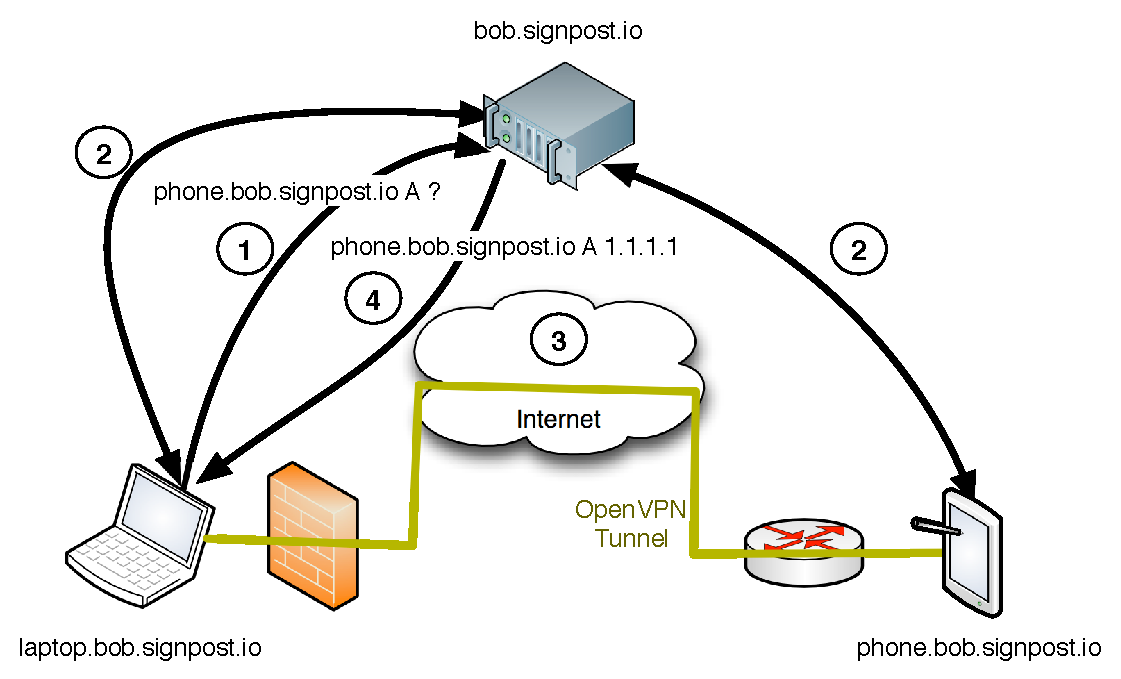
\includegraphics[width=0.6\textwidth]{Chapter3/Chapter3Figs/sp-illustration}
  \end{center}
  \caption[\signpost example use-case.]{An example use-case of the \signpost
    abstraction. Alice establishes a direct communication channel between 
    her smarthphone and her home PC over the Internet.}
  \label{fig:signpost-user-abstraction}
\end{figure}

In order to introduce the reader to the \signpost abstraction, 
Figure~\ref{fig:signpost-user-abstraction} depicts a simple use case example.  In this
scenario Alice, while at work, wishes to access
files from her laptop, situated behind a home router through her smartphone. In order to express
his interest to connect to his laptop, Alice performs a name lookup for the domain
name \fqsn{laptop.bob} to his local \signpost resolver~(step~\ding{192}).  The
name request propagates through the public DNS infrastructure to his \signpost
cloud service, which we call the {\it \signpost controller}. A verified name
request to the \signpost controller initiate the connection establishment logic
of the system, which triggers the two devices to try multiple connection
establishment mechanisms and setup an end-to-end path~(step~\ding{193}). Once an
initial path is available~(step~\ding{194}), the controller replies to the
initial name request with a local \signpost-specific IP address. Traffic to this
address is routed by the device network stack to the established inter-device
network path~(step~\ding{195}).  In parallel, \signpost continues to evaluate
different connection mechanisms, aiming to discover paths with higher
performance, and monitors path availability, thus recovering automatically
from disconnections. 

\section{\signpost Architecture}\label{sec:signpost-architecture}

\begin{figure}
  \begin{center}
	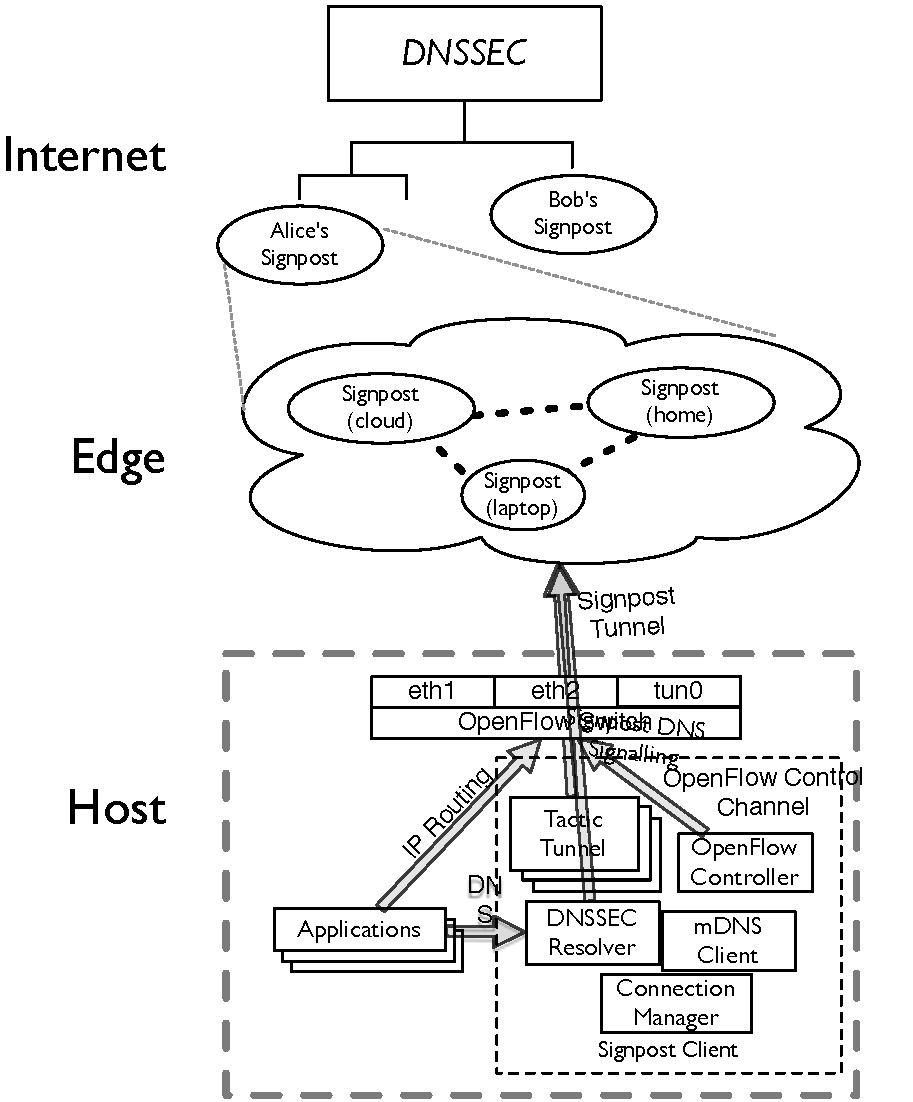
\includegraphics[width=0.9\textwidth]{Chapter3/Chapter3Figs/signpost-arch}
  \end{center}
  \caption[\signpost architecture.]{\signpost architecture over three different
    perspective: The user device, the Internet and the naming hierarchy.}
  \label{fig:signpost-arch}
\end{figure}

Figure~\ref{fig:signpost-arch} presents the architecture of \signpost over three
different viewpoints.  In the lower section of the figure, we present the design
of the \signpost software and its integration with existing applications.
\signpost logic is contained in a single executable, and requires from the guest
OS to expose a flow control abstraction, like the \of protocol, and to redirect
DNS queries to the embedded DNS resolver.  The software consists of three
subsystems: The \textit{Connection Engine}~(Section~\ref{sec:sp-engine}),
responsible to set up and manage \textit{Network
  Tactics}~(Section~\ref{sec:sp-tactics}) in order to establish end-to-end paths,
the local DNS resolver and the \of-based \textit{\signpost
  router}~(Section~\ref{sec:sp-forwarding}), which enhances the normal OS routing
functionality with \signpost network control logic.  
%%
The middle section of Figure~\ref{fig:signpost-arch}, presents the inter-device
connectivity architecture of \signpost. The system setups an Internet-wide
inter-device control channel, enabling capability and parameter negotiation
between devices. The architecture  uses a special \signpost node, which we call
\emph{\signpost Controller}, to run on a well-connected host and bridge the
device control channel across the Internet, effectively orchestrating connection
negotiation and establishment. 
%
The upper section of Figure~\ref{fig:signpost-arch} presents the naming
organisation of the \signpost architecture. The system reuses the naming
abstraction of the DNS service. Each device has a global domain name, while the
domain hierarchy and name aliasing expresses the control relationship between
devices and users.  We extend the normal name resolution functionality of the
DNS protocol and introduce an \textit{Effectful name resolution} functionality
for \signpost-enabled domains; a name resolution expresses user interest to
connect to another device and triggers the test and setup of a network
path~(Section~\ref{signpost-naming}).  The rest of the section we present in
detail the architecture of the \signpost system using a bottome-up narration. 

\subsection{Network Tactic} \label{sec:sp-tactics}

\begin{table*}
\centering \footnotesize
\begin{tabular}{|l|c|c|c|c|c|c|p{1.5cm}| }
  \hline
  Tactic name & Purpose & Layer & Transport & Authenticate & Encrypt &
  Anonymize & \signpost
Support\\
 %% & Comment & Source \\
\hline
Avahi       & Discover         & 7      & UDP         & No     & No     & No & Yes\\
 %% & Linux-based, bonjour-compatible system for local network resource discovery
 %% & \url{avahi.org/} \\
Samba       & Discover         & 7      & UDP         & No     & No     & No & No \\
 %% & Windows local network resource discovery protocol, implemented in WINS & \\
Bonjour     & Discover         & 7      & UDP         & No     & No     & No & Yes\\
 %% & Used for local network resource discovery
 %% & \url{developer.apple.com/opensource/} \\
Universal PnP & Discover         & 7      & UDP         & No     & No     & No & Yes\\
dns2tcp     & Tunnel             & 7      & UDP         & No     & No     & No & No \\
 %% & IP over DNS & \url{www.hsc.fr/ressources/outils/dns2tcp/index.html.en} \\
DNScat      & Tunnel            & 7      & UDP         & Yes    & No     & No & No \\
 %% & VPN with PPP & \url{tadek.pietraszek.org/projects/DNScat/} \\
HTTP-Tunnel & Tunnel            & 7      & TCP         & No     & No     & No & No \\
 %% & uses HTTP & \url{www.nocrew.org/software/httptunnel.html} \\
iodine      & Tunnel            & 7      & UDP         & Yes    & No     & No & Yes\\
 %% & IP over DNS & \url{code.kryo.se/iodine/} \\
NSTX        & Tunnel            & 7      & UDP         & No?    & No     & No & No\\
 %% & IP over DNS. Deprecated. Recommends iodine 
 %% & \url{thomer.com/howtos/nstx.html} \\
% IMAP        & Data transfer     & 7      & TCP         & Can be & Can be & No \\
 %% & & \\
Proxytunnel & Tunnel            & 7      & TCP         & Can be & Can be & No & No\\
 %% & can use both HTTP and HTTPS & \url{proxytunnel.sourceforge.net/} \\
ptunnel     & Tunnel            & 4      & ICMP        & Yes    & No     & No & No\\
tuns        & Tunnel            & 7      & UDP         & Yes    & No     & No & No\\
 %% & IP over DNS. Doesn't split IP packets, but sets size so small that OS does
 %%   fragmentation. Neat. Only uses CNAME for maximum compatibility with
 %%   infrastructure. Poor performance :( 
 %% & \url{www.loria.fr/~lnussbau/tuns.html} \\ 
SSH         & Tunnel/Encrypt & 7      & TCP         & Yes    & Yes    & No & Yes\\
IPSec       & Tunnel/Encrypt & 3 (4*) & IP          & Yes    & Yes    & No & No\\
 %% & In layer 4 when traversing NATS (over UDP or TCP) & \\
OpenVPN     & Tunnel/Encrypt & 7      & UDP/TCP     & Yes    & Yes    & No & Yes\\
 %% & & \url{openvpn.net/} \\
libjingle   & Nat punch         & 7      & UDP/TCP     & Yes    & Yes & No & No\\
 %% & For punching holes. Negotiation over XMPP
 %% & \url{code.google.com/apis/talk/libjingle/index.html} \\
privoxy     & Anonymize         & 7      & TCP         & No    & No   & Yes & Yes\\
tor         & Anonymize         & 7      & TCP         & No     & Yes & Yes & Yes\\
 %% & & \url{www.privoxy.org} \\
% SMTP        & Data transfer     & 7      & TCP         & Can be & Can be & No \\
stunnel     & Encrypt        & 7      & TCP         & Yes    & Yes    & No & No\\
TCPCrypt    & Encrypt        & 4      & TCP         & No     & Yes    & No & No\\
\hline
\end{tabular}
\caption[List of available connection establishing
mechanisms.]{\label{tbl:signpost-tunnels}List of available connection
  establishing mechanisms. The table presents for each mechanism, its primary
  functionality, the layer providing connectivity and the protocol used to
  establish connectivity and the support of the mechanism for Authentication,
  Encryption, Anonymisation and \signpost integration.}
\end{table*}

In order to provide end-to-end connectivity, \signpost reuses available
functionality from the wide range of free and open source connection
establishing mechanisms. Table~\ref{tbl:signpost-tunnels}, presents a survey of
such mechanisms along with their network requirements and security properties,
highlighting significant diversity between available mechanisms.  For example,
some mechanisms provide connectivity, bypassing strict network policies,  other
mechanisms enhance security and privacy in end-to-end Internet paths, while a
third class enables connection automation.  Furthermore, available mechanisms
vary significantly on the operating network layer and the exposed connection
abstraction. Connection mechanisms expose connectivity over a specific transport
layer port or through a network layer device.  In terms of protocols, the
majority uses UDP or TCP sockets, but some mechanisms use other network
protocols, like ICMP\@.  Finally, authentication exhibits significant diversity,
spanning from user-based authentication, using either passwords or certificates,
to simple pre-shared passphrases, while some mechanisms lack support. 

\begin{figure}
  \begin{center}
	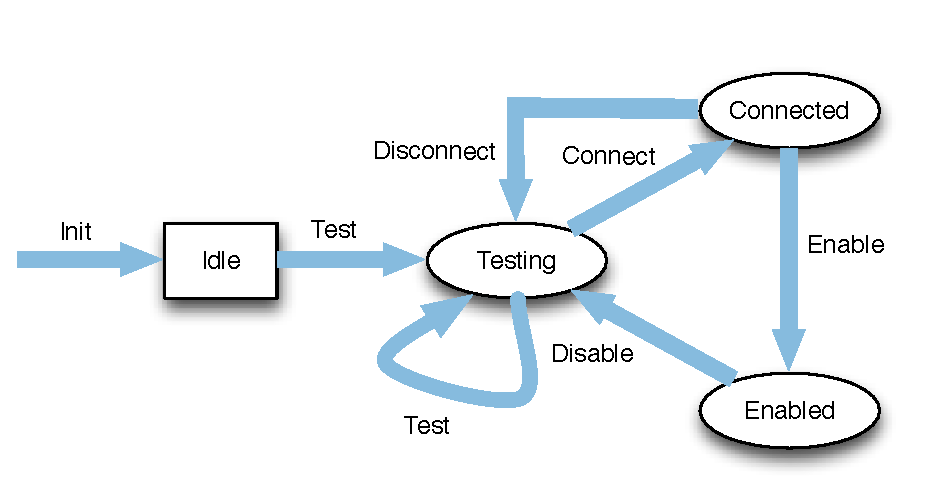
\includegraphics[width=0.8\textwidth]{Chapter3/Chapter3Figs/signpost-tactic}
  \end{center}
  \caption{\signpost Tactic lifecycle.}
  \label{fig:signpost-tactic}
\end{figure}

In order to accommodate the variances between available connection establishing
mechanisms, \signpost defines a \textit{Network Tactic} abstraction; a generic
model encapsulating testing and control requirements and automating the
end-to-end path setup process for a connection mechanism.  A Network Tactic is
modelled as a 4 state automaton for each pair of devices, presented in
Figure~\ref{fig:signpost-tactic}.  A Tactic is initialized in the \emph{Idle}
state.  A test method invocation transfers the Tactic to the \emph{Test} state
and triggers Tactic-specific connectivity tests to discover the network policy
and configuration requirements.  If testing is successful, the Tactic can
progress to the \emph{Connected} state through an invocation of the connect
method, responsible to configure the underline Tactic to provide an end-to-end
path. Once the end-to-end path is established, the Tactic can progress to the
\emph{Enabled} state and forward traffic between the two devices over the path.
Finally, the Tactic abstraction provides methods to backtrack from each state,
tearing down any established path. 
% In order
% to avoid packet reordering, \signpost permits the parallel existence of multiple
% connected tactics for a set of devices, but a single path can be enabled at
% any point.

Furthermore, because \signpost Tactics require inter-device synchronisation and
state distribution, their functionality is distributed between the \signpost
controller and \signpost devices and split logically in two layers: the
\emph{Southbound layer}, implements low-level Tactic operations and runs on
\signpost clients, and the \emph{Northbound layer}, implements the state
transitions of the Tactic automata, translating them into low-level operations,
and runs on \signpost controllers. 

The two layers of a Tactic employ the control channel between the devices and
the \signpost controller to communicate using a JSON-RPC
service~\mycite{jsonrpc}.  The control channel is exposed as a TCP service on
port 5353.  \signpost requires a control channel with high availability to
ensure Tactic parameter negotiation, even in heavily policed networks.  If
direct connectivity fails, the system uses as a fallback mechanism an
Iodine~\mycite{iodine} DNS tunnel. Iodine uses the DNS protocol to transmit data
between two hosts on UDP port 53, by encapsulating tunnel traffic in well-formed
DNS packets which can travel through recursive DNS resolvers. Iodine can provide
connectivity as long as the naming service, an important service for Internet
connectivity, is not blocked in the network. The choice of Iodine provides
sufficient capacity and latency to support the \signpost control channel, while
better integration of control messages with the DNS packet format can improve
the channel performance. 

In order to present the separation between the two layers, we present the
implementation details of the  \openvpn Tactic test method. For the specific
functionality, the Southbound layer of the Tactic provides two operation: the
\textit{init} operation, initializing an \openvpn server, and the \textit{test}
operation, testing client connectivity to an \openvpn service. The Northbound
test method uses the Southbound operations to evaluate connectivity between two
devices. During connection testing between two devices, the test method will in
parallel execute on both device initially the init operation and then the test
operation toward the other device.  The first device returning a successful test
result becomes the client of the \openvpn tunnel.  If the test times-out or both
devices return a negative result,  then the controller will initialise a local
\openvpn server and execute the test operation on both devices towards the
controller.

\subsection{Forwarding} \label{sec:sp-forwarding}

\signpost exposes connectivity on the network layer of the host, thus achieving
backwards compatibility with existing decentralized applications. A \signpost
cloud is abstracted as a local subnet and each device is assigned a persistent
local IP\@. An ARP proxy, integrated with the \signpost software, 
replies with the MAC address \texttt{fe:ff:ff:ff:ff:ff}\/ to all \signpost-local
IP addresses, thus reducing broadcast traffic and focusing forwarding decisions
on the network layer.  \signpost relies on programmable network control
mechanisms, like the \of protocol, to dynamically define forwarding policy and
detect connection problems.

The majority of the \signpost control logic is defined by Network Tactics.
Non-\signpost traffic is forwarded based on the routing configuration of the
host.  For \signpost traffic, control is delegated to Tactics, which are
responsible to install appropriate forwarding rules.  Tactics can inject and
intercept traffic and exercise control proactively or reactively.
section~\ref{sec:sp-implementation} presents the  integration details between
the \signpost architecture and connection establishing mechanisms and elaborate
on different network control approaches.  

\subsection{Connection Manager} \label{sec:sp-engine}

\signpost Tactic management is implemented by the \textit{Connection Manager}
module.  The module runs on the \signpost controller, controlling path
establishment, selecting optimal paths between device pairs and ensuring
connectivity.  Path establishment uses the Tactic abstraction to isolate
low-level connection details.  In terms of path selection, \signpost can
establish multiple end-to-end paths between two devices, but multipath
connectivity is not supported by popular transport protocols, while newer
multipath-enabled protocols, like SCTP~\mycite{RFC3286} and multipath
TCP~\mycite{RFC6824}, are not yet available in production systems.  As a result,
\signpost can use only a single end-to-end path between each pair of devices.
Path search is initiated by the connect method of the Connection Manager module,
with parameters the device names and a list of security properties. Path
selection takes under consideration two aspects: performance and security
properties.  

Path performance in \signpost reflects the resource availability in a path. The
current implementation of \signpost uses a set of simple and static heuristics
to predict path performance, based on the properties of the underlying Tactics.
More specifically, Tactics using the \signpost controller as a path relay exhibit
lower performance in comparison to direct paths, while Tactics using
connectionless protocols, like UDP, are considered more efficient than Tactics
using connection-oriented protocols, like TCP\@.  These simple rules provide an
approximation of the Tactic performance.  Path performance characterisation can
also incorporate active network measurements to improve flexibility and
estimation accuracy. 

In terms of security properties, \signpost considers three elementary
functionalities for each Tactic: \textit{encryption}, \textit{authentication}
and \textit{anonymity}.  An encrypted Tactic applies strong cryptography on both
directions of the path, while an authenticated Tactic uses strong authentication
during the establishment of the path.  Finally, an anonymising Tactic provides
built-in user identity obfuscation on the path.  Each Tactic provides a subset
of these functionalities, based on the capabilities of the underlying connection
mechanism (Table~\ref{tbl:signpost-tunnels}), and there is no single Tactic
supporting all security properties and ensuring connectivity under any network
environment. In order to address this limitation, \signpost defines a
\textit{Tactic synthesis} operation; a path can be constructed by layering
multiple connectivity mechanisms and effectively creating a path providing the
aggregate security properties. For example, an anonymised and authenticated path can
be established using an SSH tunnel over a TOR circuit between the two devices.
It is important to point out at this point that \signpost uses existing
frameworks to enhance security for an end-to-end path and does not develops a
security framework from scratch. The security properties of a path are a side
effect of the used Tactics.  End-users can use security properties to define
security policies towards specific devices. The policy is expressed through a
configuration file and users specify security requirements on a per domain
basis. 

Path selection is modelled as a dynamic optimization problem with security
requirements modelled as constraints and path performance modelled as the
objective function.  Path performance is represented by a positive integer
weight, with higher values reflecting lower performance of the path. The weight
of a path is equal to the sum of the individual weights of the Tactics
synthesizing the path.  Path selection uses a Breadth-first search mechanism
over the complete space of all possible Tactic combinations.  During a
connection request the system spawns a thread for each Tactic, testing
end-to-end connectivity.  If the test is successful, the Tactic will try to
connect the two hosts. If the connection is also successful and either there is
no other Tactic enabled or the enabled Tactic has a higher performance value,
then the Manager will progress the state machine of the Tactic to the
\emph{Enabled} state and disable any existing enabled Tactics. If the Tactic
doesn't fulfil the security policy, the Manager will recursively try to layer
more Tactics over the established path and find a Tactic synthesis with
sufficient security properties. The Manager returns a successful result when the
algorithm finds a path configuration fulfilling the security policy, but the
search will continue to search for better paths.  The search will terminate when
all remaining Tactic combinations have a higher performance weight or they are
synthesized by more that three Tactics.  Effectively, the search algorithm
establishes rapidly a first path between two devices and progressively optimize
path performance, while the devices remain interconnected. 

Finally, the connection manager  module is additionally responsible to monitor
enabled paths and detect disconnections. The module uses \texttt{flow\_stats}
\of messages to identify packet transmissions during a monitoring period, and
thus infer path liveness. If the path is idle during that period period, the
module uses a UDP heartbeat service, to verify path connectivity. During a
heartbeat timeout, the connection manager tears down the path and repeats the
path search  process.  A Tactic can employ application-specific
connectivity evaluation mechanisms, e.g. \openvpn provides a keep-alive mechanism. 

\subsection{Effectful Naming} \label{signpost-naming}

The majority of Internet-connected devices are essentially anonymous from a
network perspective, being assigned transient names (e.g.,~via DHCP). The IPv6
protocol~\mycite{RFC1883} addresses a number of such limitations, but the protocol
deployment on the edges of the Internet has been slow and limited. A fundamental
goal for the \signpost architecture is to support stable and secure resolution
of device  names to concrete end-to-end paths.  \signpost uses the DNS
protocol~\mycite{RFC1034} to support its naming functionality for two reasons.
Firstly, DNS is an effective solution for the naming problem. It is an
Internet-wide service, supported by all network applications and never blocked
in a network. The introduction of the \dnssec protocol extensions provides
additional bi-directional authentication.  Secondly, the DNS service supports
inherently delay-tolerant service indirection, used extensively across the
Internet.  Many services employ user-friendly domain names to represent virtual
service end-points which are refined during name resolution, directing user to
the best service mirror based on the end-host location and the service
load~\mycite{RFC3568}. Effectively, a domain name resolution represent the
interest of a user to connect to a service, which the service provider can
direct to a concrete end-point based on the network context.  

The Internet naming service provides good scaling properties, using a
hierarchical architecture. Every domain name consists of a sequence of name
tokens organised in a hierarchical tree structure with a single root, the empty
string. Every node on the tree can be coupled with a number of DNS Resource
Records (RR) and provide rich information for the domain name, like its network
addresses and name aliases. In order to scale the performance of the naming
service across the Internet, the design of the system allows service delegation
for a zone to other servers using the NS RR type.  In addition, the DNS
service defines a record caching mechanism, to improve lookup performance and
service load. 

A DNS packet (queries and responses)  contains a standard header and four
sections: the \emph{question}, containing the name being looked up; the
\emph{answer}, containing RRs answering the question; the \emph{authority},
pointing to an authoritative server for the question; and the \emph{additional}
records, containing any additional information pertaining to the question. Name
resolution then follows one of two paths. A \emph{recursive resolution} occurs
when the server does not have the answer and so it acts as a resolver itself,
pursuing the answer on behalf of the client. In contrast, an \emph{iterative
  resolution} occurs when the server does not have the answer and responds by
referring the client to a server ``closer'' to the answer.

\signpost reuses the DNS naming service abstraction and extends its
functionality, introducing the idea of \textit{Effectful name resolution}.
Effectfull name resolutions have as a side-effect  the creation of an end-to-end
path towards the requested destination.  Effectively, \signpost perceives name
resolutions as an intention to connect to the requested device and translate the
name resolution in an explicit connection request to the Connection Manager
module. This extension to DNS functionality is similar to the indirection
functionality of the protocol. In addition to pointing the requester to an
appropriate network adress, \signpost ensures a path towards that address. 

% \begin{itemize}
% \item\emph{Ubiquity}. DNS is among the most widely deployed services on the
%      Internet. Effectively every Internet-connected client supports name
%      resolution, and has access to the DNS when connected. 
% \item\emph{Reach}. As such a critical part of the Internet's infrastructure, and
%      unlike TCP, HTTP and similar protocols, DNS tends not to be manipulated by
%      middleboxes other than modified DNS servers
%      themselves~\mycite{rfc:3234,handley-mbox}.
% \item\emph{Security}. The DNSSEC security extensions have recently been deployed
%      on the live root servers~\mycite{rfc:4033}.  DNSSEC provides origin
%      authentication and integrity protection for DNS records, and (along with
%      SSL) represents one of the two global public key infrastructures.
%    \end{itemize}

% Details of the DNS protocol can be found in RFC 1035~\mycite{RFC1035} and its
% many extensions and updates in the RFC repository. Before we discuss Signposts
% in detail, it is necessary to briefly recap key elements of DNS.

\paragraph{Secure Names For All Internet Users}

\begin{figure}
  \centering
    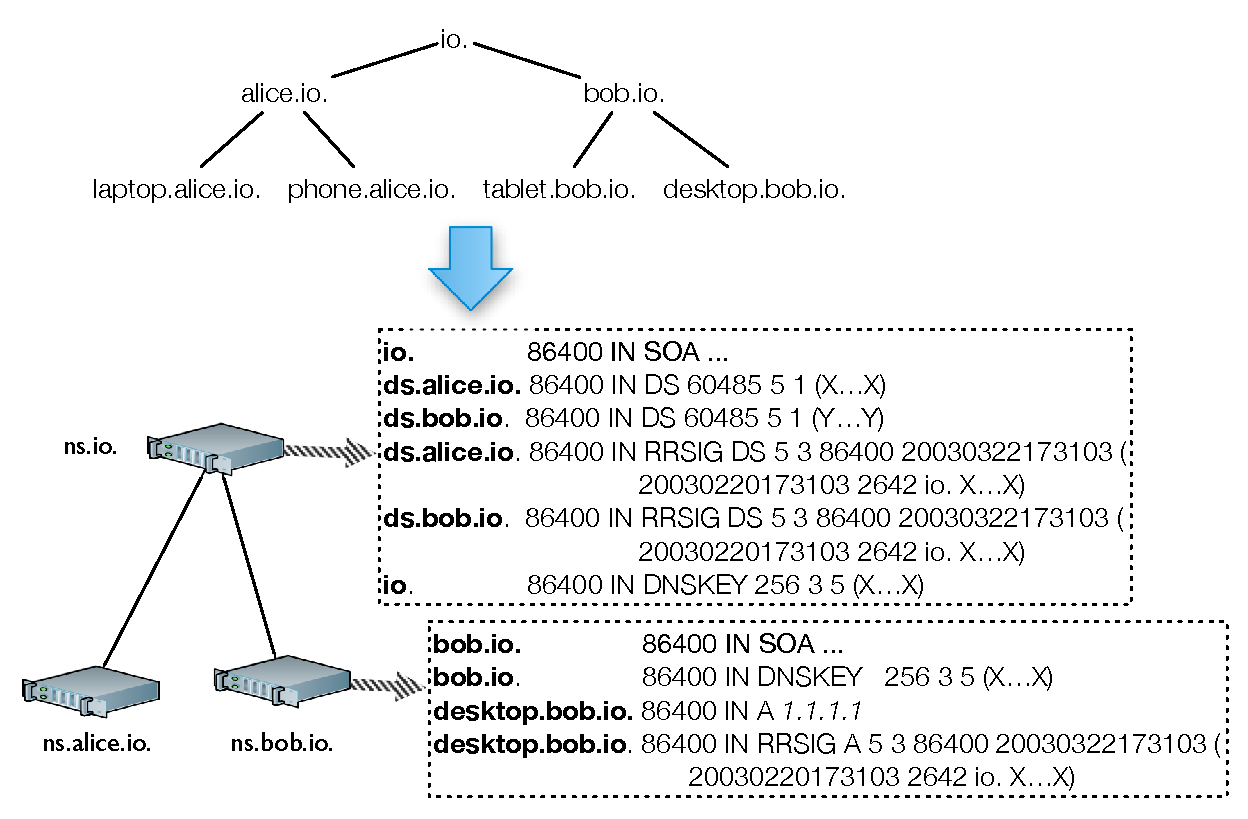
\includegraphics[width=0.9\textwidth]{Chapter3/Chapter3Figs/DNSSEC_hierarchy}
    \caption[Example \dnssec zone files.]{Example \dnssec zone files for the
      \spsn{signpost.io} and \fqsn{bob} domains. The \spsn{signpost.io}
      nameserver zone file contains a DS RR with the hash of the bob.io.  DNSKEY
      RR and an RRSIG RR signature of the DS RR signed with the DNSKEY of the
      \spsn{signpost.io} domain. \fqsn{bob} uses its DNSKEY to sign an A RR for
      \fqsn{desktop.bob}}
  \label{fig:dnssec_hierarchy}
\end{figure}

The initial definition of the Internet naming service provided weak security
guarantees and was vulnerable to man-in-the-middle and cache
poisoning~\mycite{DNSPoisonning} attacks.  In order to enhance the security
primitives the IETF standardised a number of DNS protocol extensions, described
as \dnssec.  \dnssec defines three RR types~\mycite{RFC4034}, enabling response
authentication as presented in Figure~\ref{fig:dnssec_hierarchy}.  In \dnssec,
each zone owns one or more cryptographic keys to sign authoritative DNS
responses. The \dnssec extensions define four new DNS RR types to accommodate
the authentication functionality. The RRSIG RR type can carry RR signatures,
while the NSEC RR type reflects the lack of specific RRs for a domain to a
resolver.  The DNSKEY RR type disseminates public keys of a domain to resolvers,
which in turn can use them to authenticate response signatures. Finally, the DS
RR type expresses the trust of a domain to a signing key of another domain. With
respect to Figure~\ref{fig:dnssec_hierarchy}, the domain \fqsn{bob} signs an A
record for the host \fqsn{desktop.bob} through an RRSIG RR using Bob's DNSKEY\@.
Bob's key is registered with the \spsn{signpost.io} domain through a DS RR, containing the
hash of the key and signed using an \spsn{signpost.io} public key.  Effectively, the \dnssec
extensions form a chain of trust as part of the naming service and ensure
query response and key authenticity. The resolver requires, as in the X509
certificate architecture, only a list of authenticated anchors, configured
out-of-band and injected in the authentication chain.

\signpost uses the \dnssec RR types to establish an authenticated control
channel between the devices of the user. Each \signpost user must have
authoritative control of a domain zone, serviced by the \signpost controller,
and register a signing key to the \dnssec chain of trust. Each device has a
domain name under the domain  of the user. With respect to
Figure~\ref{fig:signpost-arch}, Bob is granted control of the zone \fqsn{bob}
where he registers his laptop under the domain name \fqsn{laptop.bob}. As a
result, each \signpost user has a globally accessible authenticated public
identity for each device via a public-private key-pair. Using this key-pair, a
user can sign and authenticate messages, bootstrap public key cryptography
mechanisms and run key-exchange mechanisms such as
Diffie-Hellman-Merkle~\mycite{RFC2631} and derive new shared private keys
between any two devices over unsecure channels.

The base \dnssec RR types  provide a mechanism to authenticate responses from a
nameserver to a DNS resolvers. In terms of the \signpost architecture, we are
interested additionally to authenticate DNS requests. Authenticated requests
enable the server to present a different view over the resource mappings,
depending on the querying entity\footnote{{\em ``DNS servers can play games.  As
    long as they appear to deliver a syntactically correct response to every
    query, they can fiddle the semantics.''---\,RFC3234~\mycite{RFC3234}}}.
\signpost uses the SIG(0) RR type, defined in~\mycite{RFC2931}, to sign DNS
requests using the key of the device.  
% The record was introduced in order to allow authorized
% clients to update RR records on an authoritative server, while it permits a
% client also to point to the signing entity, in order to fit the authentication
% within the \dnssec key structure. 

% Using DNSSEC here instead of SSL has several important advantages. Firstly,
% DNSSEC has maintained the integrity of its trust chain better than SSL (which
% has a large set of root certificate providers), and has explicit support for
% incomplete trust chains via look aside validation~\mycite{RFC5074}.  Secondly,
% DNSSEC has few network dependencies and exploits all of the distributed benefits
% of DNS, such as caching, proxy lookups, and a low-latency protocol.  Lastly, a
% domain also has a single, well-defined owner if registered under a top-level
% domain, whereas URL-based identity schemes such as
% OpenID~\mycite{Recordon:2006:OPU:1179529.1179532} depend on trusting the
% underlying owner of the domain for that URL.\todo{will we discuss icann
%   implications of so many new internet names later on?}

%% \subsection{Centralised Named Routing}
%% \label{s:topo1}

\paragraph{\signpost integration with \dnssec} 

\signpost evolves the \signpost client and controller DNS functionality.
Specifically, the controller runs a programmable DNS service, which is
authoritative for the user domain. The server serves is authoritative for the
user domain,  signs responses on-the-fly, verifies SIG(0) signed queries and
translate them into Connection Manager requests. A request for an A RR for
domain name \fqsn{laptop.alice}, signed with a SIG(0) record with a key from
host \fqsn{desktop.alice}, will be translated into a connection request between
Alice's laptop and desktop devices.  
% In order to enforce liveness of \signpost
% RR records in the Internet, we set a zero TTL value on all RR records, thus
% disabling any DNS caching.
In the client side of the \signpost architecture, we use a local \signpost-aware
DNS resolver. DNS queries for non-\signpost hosts trigger a recursive search of
the DNS name tree, in order to retrieve the requested RRs.  For \signpost 
requests, the resolver sings the query with a SIG(0) record using the private
key of the device. 

The DNS functionality provides additionally offline in a local network.
Specifically we use DNS-based service discovery~(DNS-SD)~\mycite{RFC6763}, an an
RR organisation specification which enables service advertisement and browsing
in a local network. DNS-SD uses the Multicast-DNS~\mycite{RFC6762} service and
provides an efficient local service discovery mechanism. The combination of
DNS-SD and multicast-DNS is currently a popular service discovery mechanism in
local networks, supported by most operating systems.  The \signpost system
advertises, using the DNS-SD mechanism, a \signpost service record with name
\spsn{\_sp.\_tcp.local} along with an RRSIG RR and the DNSKEY RR of the device,
signed with the private key of the user domain. Another \signpost client can
verify a destination \signpost service, using a locally cached copy of the
\signpost controller public key, and establish a control channel.  In offline
mode, a query receiver functions as a \signpost controller, responsible to
server RR request for its domain name only. 

\subsection{Security and Key Management} \label{signpost-security}

\signpost extends the \dnssec protocol architecture to develop a public key
distribution mechanism.  Firstly, \dnssec exhibits better trust chain integrity
in comparison to SSL, which has a large set of root certificate providers, and
supports incomplete trust chains via look aside validation~\mycite{RFC5074}.
Secondly, a domain in \dnssec has a single, well-defined owner, registered under
a top-level domain, whereas URL-based identity schemes, like
OpenID~\mycite{Recordon06}, is subject to the trust to the domain owner.

\signpost key hierarchy extends the \dnssec key hierarchy and introduces an
additional layer of device keys in each user domain. \dnssec deployment
specifications dictate the use of at least two RR signing keys~\mycite{RFC4641}: A
\textit{Zone Signing Key (ZSK)} and a \textit{Key Signing Key (KSK)}.  ZSK signs
the KSK, and its hash is stored as a DS RR in the top-level zone.
KSK is used by the controller to sign authoritative RRs\@.  The
use of two keys by the authentication mechanism provides a
persistent anchor in the \dnssec key hierarchy for each domain and enhances
flexibility in key revocation; KSK rollover requires only a few record
modification in the zone file.  \signpost introduces an additional layer
of \textit{Device Signing Keys (DSK)}, which are signed using the KSK and used
by the devices to bootstrap authentication.  In order to join a Personal Cloud,
a device must generate a DSK and add it in the zone file of the \signpost controller
using a DNSKEY
RR and a signed RRSIG RR. Any device with an anchor in the global \dnssec key
infrastructure can verify any \signpost signed request, by following the key
chain in the \dnssec tree.

\section{Evaluation}\label{sec:signpost-evaluation}

In this section we evaluate the \signpost system and its compatibility with
distributed Personal Cloud applications.  Specifically, we
present a strawman \signpost implementation and its integration with a set of
Tactics (Section~\ref{sec:sp-implementation}), we measure the performance of the
available \signpost Tactics in a realistic testbed
(Section~\ref{sec:sp-tactic-eval}) and we discuss the experience in the
integration of \signpost with a set of popular applications
(Section~\ref{sec:sp-compatibility}). 

\subsection{\signpost implementation} \label{sec:sp-implementation}

\signpost is implemented predominantly in OCaml, a type-safe functional language
providing enhanced security and fast prototyping.  The implementation uses
existing protocol libraries to integrate DNS and \of programmable protocol
support to the core daemon of the system.  Our strawman implementation is fully
functional under Linux and Android, using the \ovs switch implementation, and
MacOSX, using a userspace switch implementation from the ocaml-openflow library.
Our \signpost implementation supports  the following connection establishing
mechanisms: 

\begin{itemize}

  \item \emph{Direct}: The Direct Tactic evaluates the
    ability of  two devices to connect directly without any
    tunnelling mechanism. The Tactic test method evaluates if direct
    bi-directional connectivity is possible between the two devices on a set of
    well-known service ports (e.g. TCP and UDP connectivity on ports 53, 80, 443
    and 8080). If the tests are successful, the Tactic inserts \of
    rules on both devices to translate \signpost addresses to 
    network addresses. 

  \item \emph{\openvpn}: The \openvpn Tactic integrates the
    respective tunnelling mechanism with the \signpost architecture. The Tactic
    test method evaluates inter-device and device-\signpost controller
    connectivity on UDP port 1194. The Tactic connect method uses the
    \signpost keys to bootstrap the \openvpn authentication mechanism.  Because
    of some limitation in OpenSSL certificate chain evaluation, for each path
    the Tactic generates transient private keys, signed by the user private key,
    and injects in the trusted certificate configuration of the \openvpn
    software a certificate for the destination device key signed by its private
    key.  The Tactic configure the \openvpn software to expose connectivity
    through
    an Ethernet TAP interface~\mycite{tuntap}, which is added to the local
    switch datapath. Each TAP device is assigned an IP in the 10.0.0.0/16 subnet
    and appropriate ARP announcement packets are broadcasted, to bootstrap state
    in the internal \openvpn ARP cache. Finally, The Tactic enable method
    inserts \of rules to forward packets over the \openvpn tunnel and translates
    source and destination addresses, similarly to the direct Tactic. 
%     rules establish full bi-directional connectivity.  
%     \todo{Mention OpenVPN ARP cache}

  \item \emph{SSH}:  The SSH Tactic provides inter-device connectivity using the SSH
    protocol. The Tactic configures and runs an SSH server on every \signpost
    device on port 10000, configured exclusively to provide tunnelling
    functionality using key-based authentication. We spawn a separate SSH
    daemon on each device, to enable tighter service configuration.  Tactic
    testing evaluates direct TCP connectivity between the devices or through the
    \signpost Controller.  The connect method of the SSH Tactic appends the
    public key of the destination device in the \texttt{authorized\_key} and the
    \texttt{known\_host} SSH configuration files and uses the device private key to
    authenticate the client and server during connection.  The SSH Tactic
    associates the SSH tunnel with a local TAP Ethernet interface on each device
    and the Tactic inserts appropriate \of rules to forward traffic to the TAP
    interface.

  \item \emph{Privoxy}: The Privoxy Tactic enables HTTP request anonymisation using the
    Privoxy~\mycite{privoxy} HTTP proxy. The Tactic provides a mechanism to purge
    HTTP requests and responses from user identification elements, buts does not
    ensures connectivity guarantees. The Tactic test method
    configures a Privoxy HTTP proxy server on each device, configured with a
    strict anonymisation policy, and succeed only when the Tactic is used in a
    synthesised path and the Tactic is tested over an existing connection
    establishing Tactic (e.g.~direct, \openvpn,~etc.).  Privoxy connect method
    handles TCP flows in a proactive manner.  For each
    SYN packet, the Tactic install bi-directional flows, forwarding data from
    the application to the local listening port of the Privoxy daemon.

\begin{figure}
  \begin{center}
	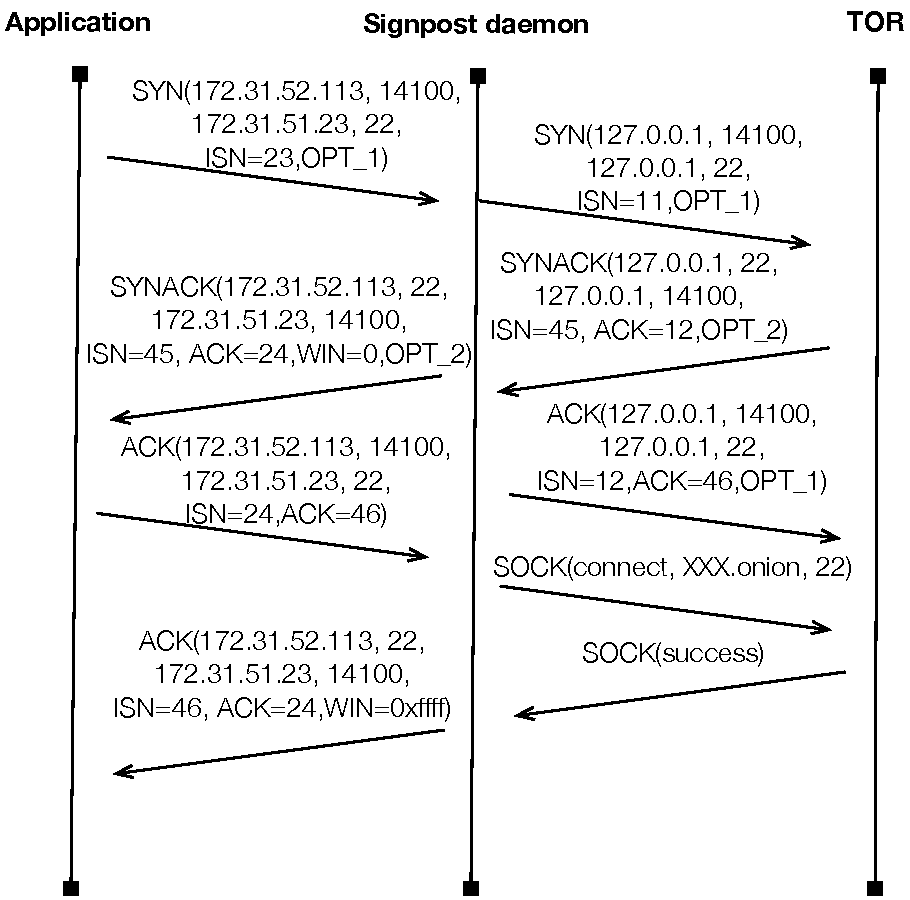
\includegraphics[width=0.7\textwidth]{Chapter3/Chapter3Figs/tor-example}
  \end{center}
  \caption[TOR Tactic connection establishment sequence diagram.]{TOR Tactic
    connection establishment diagram. The Tactic translates each
    TCP connection request to the destination device to a SOCKS
    request to the TOR proxy.}\label{fig:signpost:tor-example}
\end{figure}
  
  \item \emph{TOR}: The TOR Tactic enables connectivity between devices over the
    TOR anonymised network~\mycite{dingledine2006}. The Tactic configures a TOR
    client on each device, exposing a SOCKS proxy and uses the TOR hidden
    service functionality to support inter-device connectivity. The Tactic
    generates for each host an anonymized domain name under the \spsn{.onion}
    domain and employs the embedded name lookup capability of the SOCKS protocol
    to provide host discoverability over end-to-end TOR circuits. The TOR test
    method initializes the TOR client, propagates the domain name of the device
    to the \signpost controller and tests the effectiveness of the Tactic in the network
    environment.  
    
    The TOR Tactic uses a reactive control scheme. For each SYN packet to a
    \signpost host, the Tactic injects packets to initiate a TCP connection with
    the local SOCKS proxy and sends a SOCKS request to establish a TOR circuit
    to the destination device.  On TCP connection establishment with the local
    SOCKS proxy, the Tactic responds to the initial SYN request with a SYNACK
    packet with sequence and ACK numbers which accommodate the additional bytes
    of the SOCKS request, and a zero receive window, to suppress any further
    data transmissions from the application.  Once a positive SOCKS response is
    received, the Tactic sends to the initiating TCP flow an ACK packet with a
    non-zero window and insert appropriate \of rules to translate on the fast
    path IP addresses and port numbers.  On negative SOCKS response, the Tactic
    injects TCP RST packets to tear-down all flows.
    Figure~\ref{fig:signpost:tor-example} presents a sequence diagram of the
    Tactic interactions.  In order to replicate a similar abstraction for UDP
    and ICMP traffic, we setup a VTUN~\mycite{vtun} tunnel over TOR, thus
    enabling IP-level connectivity.  We avoid using the tunnel for TCP
    connections, to reduce header capacity losses of the tunnelling mechanism. 

  \item \emph{DNS-SD}: The DNS-SD Tactic enables service advertisement between
    \signpost devices. DNS-SD~\mycite{RFC6763} is a common OS service enabling
    hosts to advertise services in the local network.  The Tactic aids existing
    decentralised Personal Cloud applications to discover available services
    running on other \signpost devices. Similarly to Privoxy, the Tactic does
    not provide connectivity and thus can only be used in synthesized paths.
    The Tactic connect method intercepts DNS-SD packets from the network stack
    of the device and propagates them over the control channel to the other
    devices of the user.  \signpost daemons inject equivalent DNS-SD multicast
    packets through the \of protocol to the network loopback device and thus
    provide service discovery.

\begin{figure}
  \begin{center}
	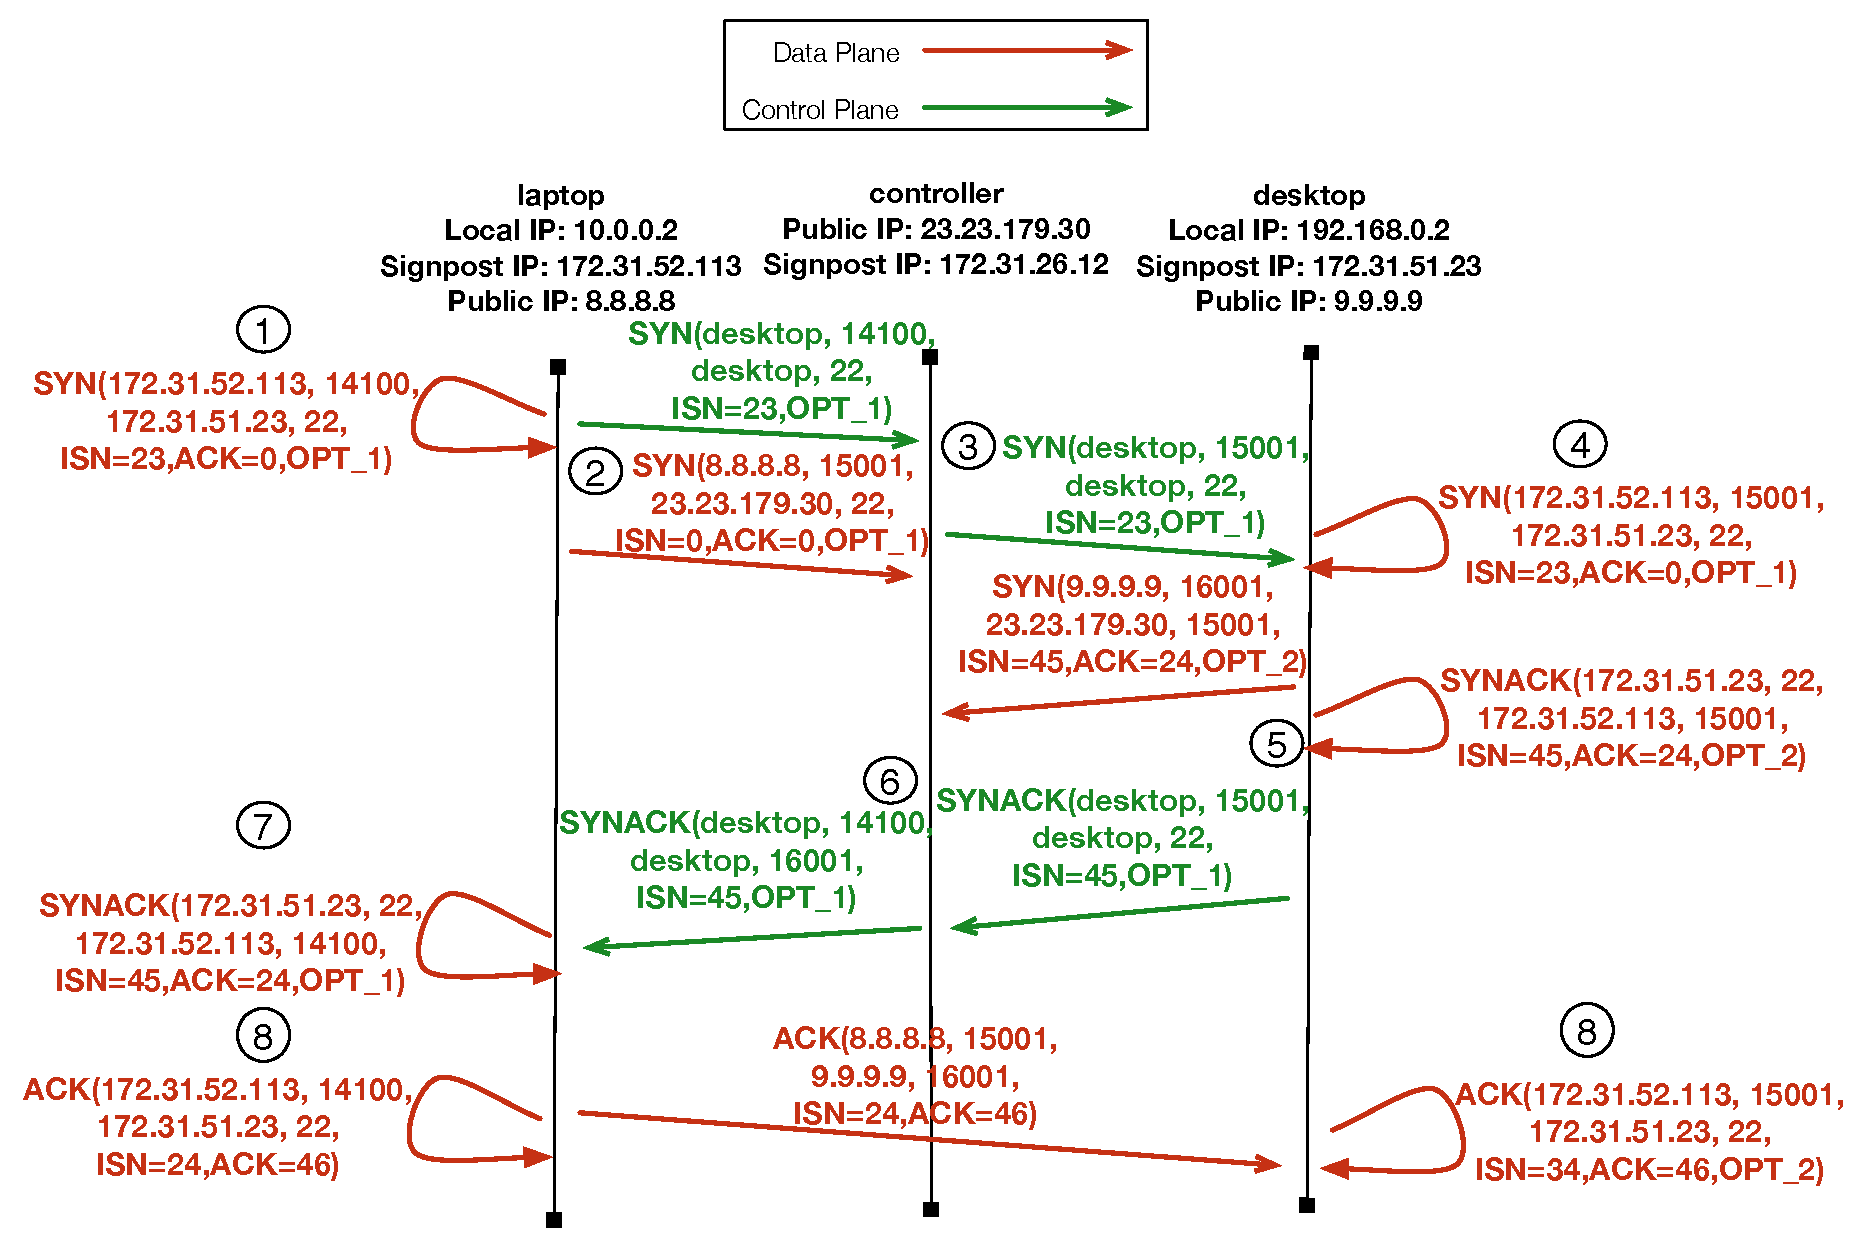
\includegraphics[width=0.99\textwidth]{Chapter3/Chapter3Figs/nat-punch-example}
  \end{center}
  \caption[NAT-punch Tactic connection establishment sequence
  diagram.]{NAT-punch Tactic connection establishment sequence diagram.The
    device \signpost daemon injects crafted packets to create appropriate state
    in the local NAT, while the controller detects the applied port mapping for
    both hosts of the \signpost path.}
  \label{fig:signpost:nat-panch-example}
\end{figure}
  
  \item \emph{NAT-punch}: The Tactic implements a packet injection technique which
    allows TCP and UDP flows to bypass NAT boxes. The Tactic supports only
    Full-cone NAT, Address-restricted NAT and Port-restricted
    NAT~\cite{RFC3489}.  The NAT-punching Tactic uses the \signpost controller to infer
    the port mappings configuration of the local NAT\@. We present a sequence
    diagram between two device and the \signpost controller to establish a TCP
    connection using the NAT-punch Tactic~\ref{fig:signpost:nat-panch-example}.
    Specifically, for a new TCP connection, the daemon intercepts the SYN packet
    (Step~\ding{192}), propagates important header fields~(Port number, initial
    sequence number and TCP options) over the control channel to the remote
    device and sends a SYN packet from the device to the \signpost controller in
    order to infer the port mapping policy and create appropriate state in the
    NAT (Step~\ding{193}). When the \signpost controller receives the SYN, it
    extracts the source port mapping applied by the NAT and forward it, along
    with the TCP initial sequence number, to the destination device
    (Step~\ding{194}).  Once the destination device receives the control message
    from the \signpost controller, it will generate a SYN packet, using the header fields
    of the initial SYN packet, and send it both to the listening service and the
    \signpost Controller~(Step~\ding{195}). In the destination device, the
    \signpost daemon intercepts the SYNACK response of the listening service and
    propagate the TCP header fields over the control channel to the connection
    initiating device~(Step~\ding{196}).  Once the exact port-mapping is
    inferred by the Controller, the information is propagate to the initiating
    device~(Step~\ding{197}), which will inject a SYNACK packet to the local
    stack to progress the TCP-handshake~(Step~\ding{198}). Finally, once the two
    device know the NAT port-mapping and have created appropriate state in the
    NAT flow table, the Tactic inserts \of rules to translate appropriately
    incoming and outgoing traffic of the flow~(Step~\ding{199}).

    For UDP traffic, the Tactic controller will intercept the initial UDP packet
    of the flow and propagate it over the control channel to the remote device,
    as well as, transmit a similar packet to the \signpost controller in order
    to generate appropriate state in the intermediate NAT services. The remote
    device sends a similar UDP packet to the \signpost controller. Once the
    controller has received both UDP packets, it will notify both devices to
    transform appropriately flow IP address and port numbers, using \of flows. 
\end{itemize}

\subsection{Tunnel Evaluation} \label{sec:sp-tactic-eval}
\begin{figure}
  \begin{center}
	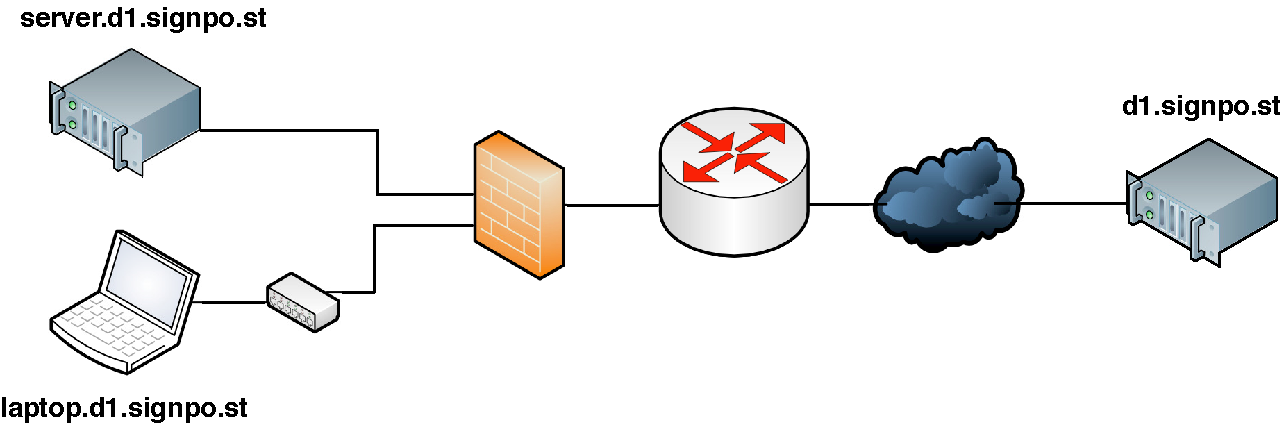
\includegraphics[width=0.9\textwidth]{Chapter3/Chapter3Figs/measurement_topology}
  \end{center}
  \caption[\signpost Tactic evaluation topology.]{\signpost Tactic evaluation
    topology. \textit{server} and \textit{laptop} hosts are connected on
    different subnets of the CL network. The laptop is connected to the network
    through a NATed home router and a stateful firewall enforces network policy
    between the two subnets.  The \signpost \textit{controller} is hosted on an
    Amazon EC2 micro instance~\mycite{ec2instances}.}
  \label{fig:signpost:measurement_topology}
\end{figure}
 
\begin{table}
\centering
\begin{tabular}{|l|>{\centering\arraybackslash}m{1.2cm}|>{\centering\arraybackslash}m{1.7cm}|>{\centering\arraybackslash}m{1.5cm}|>{\centering\arraybackslash}m{1.2cm}|>{\centering\arraybackslash}m{1.7cm}|>{\centering\arraybackslash}m{1.5cm}| }
  \hline
  \multirow{2}{*}{Tactic name} & \multicolumn{3}{|c|}{Direct connectivity} &
  \multicolumn{3}{|c|}{cloud-assisted connectivity} \\
\cline{2-7}
& setup (sec) & throughput (Mbps) & RTT (msec) & setup (sec) &
throughput (Mbps) & RTT (msec) \\
\hline
Direct       & 1.0  & 94.1 & 1.5   & -    & -     & -     \\
\openvpn     & 13.3 & 66.0 & 1.23  & 20.0 & 1.9   & 172.0 \\
SSH          & 6.8  & 86.5 & 2.73  & 8.8  & 1.7   & 829.0 \\
TOR          & 60.2 &  2.4 & 912.0 & -    & -     & -     \\
NAT-punch    & 1.2  & 94.1 & 1.5   & -    & -     & -     \\

% iperf -c quorum101.cl.cam.ac.uk  -i 1 -F /dev/urandom -t 60
% fping 172.31.28.49 -e -b 1400 -c 6000 -p 1 -D -s -e -q
\hline
\end{tabular}
\caption[\signpost Tactic performance.]{\signpost Tactic performance evaluation
  results in terms of latency to setup a path, throughput and RTT delay. Direct
  cloud-assisted paths exhibit two orders of magnitude higher performance and
  lower throughput.
\label{tbl:signpost:tactic_perf}}
\end{table}

In order to evaluate the performance of our strawman implementation, we conduct
a series of measurements for each Tactic.  Our testbed
consists of three hosts, two \signpost devices and a \signpost controller,
presented in Figure~\ref{fig:signpost:measurement_topology}. The \signpost
clients~(\fqsn{laptop.d1}, \fqsn{server.d1}) are connected to the production
network of the Computer Laboratory on different subnets through 100 MbE links.
The network enforces a security policy both between the devices and toward the
Internet using a stateful firewall.  Additionally, the host laptop is connected
to the network through a home router with NAT functionality. The \signpost
controller of our experiment runs on an Amazon EC2 micro
instance~\mycite{ec2instances}. Using \signpost, we establish all possible
end-to-end Tactics~\footnote{We exclude the privoxy and DNS-SD Tactics because
  they improve functionality on established paths only.} and measure the path
setup delay, the achievable throughput and the round trip delay for each Tactic.
More specifically, in each experiment we initialize the
\signpost daemon on each device, and establish connectivity using a specific
Tactic. For each established path we measure the delay to complete a \signpost
name resolution and initialize a \signpost path, the path throughput,
using a steady-state TCP measurement probe, and the average path RTT,
using a 1~Mbps UDP measure probe. We conduct our measurement ten times for each
possible configuration and present the medians value in
Table~\ref{tbl:signpost:tactic_perf}. 

From the result of our experiment we note the difference in capacity and latency
when a path uses the \signpost controller. Edge network connectivity provides
two to three orders of magnitude higher performance in comparison to
cloud-assisted paths.  In addition, we highlight the trade-off between security
and performance between Tactics. For example, the TOR anonymization
functionality degrades significantly the performance and latency, deeming
inadequate for responsive applications. The performance degradation is primarily
due to the onion routing scheme used to obfuscate the source and destination
addresses of the flow and the sharing nature of the system.  \signpost exposes a
clear control abstraction of the trade-off between performance and security. 

An important aspect of Tactic performance is the path setup latency. This delay
is important because the DNS protocol employs time-outs in name resolutions to
detect unresolvable domain names. Linux and OSX have a maximum delay of 15
seconds~\footnote{\url{http://linux.die.net/include/resolv.h}} (3 retries with 5
seconds time-out per request), while for windows the delay varies between 12 to
15 seconds depending on the OS
version~\footnote{\url{http://blogs.technet.com/b/stdqry/archive/2011/12/15/dns-clients-and-timeouts-part-2.aspx}}.
Bootstraping a \signpost path incurs noteworthy setup latencies but the DNS
naming service is designed to handle such latencies.  Based on
Table~\ref{tbl:signpost:tactic_perf} results, the majority of the Tactics
exhibits setup latencies within the resolver time-out limit, except the TOR
Tactic. TOR setup latency is dominated by the circuit establishment latency of
the onion overlay.  The current implementation exposes the setup latency to
applications and thus may experience DNS name lookup timeouts for the first flow
of a path. An optimistic approach can mitigate potential resolver time-outs
(e.g.~use of DNS aliases to delay the response). It is important at this point
to clarify that the measured setup latencies occur only for the first flow
of a path and subsequent flows will experience name resolution delays
equal to the round-trip time to the \signpost controller. 

Finally, using the aforementioned topology we also measured the performance of
Tactics synthesis. The results of the experiments report that the throughput and
RTT of such paths is equal to the minimum value between the Tactics forming the
network path, while the setup latency is equal to the sum of the individual
Tactics. 

\subsection{Application compatibility} \label{sec:sp-compatibility}

In this section we evaluate the compatibility of \signpost with applications
providing resource and information sharing. Our evaluation focuses on the
effectiveness of \signpost integration with such applications.  We use the
topology in Figure~\ref{fig:signpost:measurement_topology} and consider two
primary classes of applications: \emph{File Sharing} and \emph{Resource
  sharing}.  In terms of file sharing we test three popular applications, namely
the Linux NFS implementation~\mycite{RFC5661}, git-annex~\mycite{git-annex} over
rsync and SSH Secure Copy.  In terms of resource sharing we tested the
functionality of CUPS remote printing, DAAP media sharing, VNC remote desktop
and SSH remote access. 

We report that all applications function correctly from a network perspective
over all Tactic configurations. Nonetheless, user-perceived performance is
proportional to the underlying Tactic performance
(Table~\ref{tbl:signpost:tactic_perf}).  Some Tactics incur significant RTT
delays and impact the user-experience in reactive applications. For example, the
SSH software exhibited significant responsiveness problem when routed over
TOR\@. In addition, through the integration testing we identified limitations in
the openness of our architecture and modified accordingly our implementation.
For example, we observed that the Linux SSH client and server use different
values for the ToS bits, depending on the payload of the packet, and require the
respective \of rule to wildcard the ToS field value in the NAT-punch and TOR
Tactics. Our design choice to integrate \signpost with existing network
applications in the network layer of the OS is effective and enables seamless
integration with existing network applications.

\section{Summary} \label{sec:signpost-conclusion}

This chapter focused on the problem of Internet-scale inter-device connectivity.
Our work is motivated by the end-user requirement for resource and information
sharing services using network device federation between its personal devices; a
generic abstraction which we term Personal Cloud. We elaborated on the available
mechanisms and highlighted trade-offs between available solutions. We identified
a significant connectivity and naming problem in the current Internet
architecture.  We argued that the abundant of connection establishing mechanisms
provides a sufficient toolset to connect devices across the Internet, but
requires a distributed control framework to orchestrate the automatic
establishment of end-to-end path using these mechanisms. We presented \signpost,
a distributed naming and connectivity framework which enables global device
naming,  automates the testing and  configuration of end-to-end paths and
provides secure and backwards-compatible connectivity to existing network
applications. 

\signpost evolves two aspects of user device control plane. Firstly, the control
plane is extended to accommodate \textit{Network Tactics} functionality;
mechanisms enabling ad-hoc end-to-end connectivity, like tunnelling software and
NAT punching techniques. The architecture develops a generic model coupled with
a secure and high-availability Internet-wide control channel, enabling
inter-device Tactic testing and configuration orchestration.  In addition, the
rich security properties provided by existing network Tactics, allow the system
to expose a security control abstraction, providing trade-off control between
performance and security.  Secondly, the architecture integrates the control
plane logic with the naming service. \signpost provides Internet-wide
persistent device names and a global and secure key distribution mechanism,
building on top of the \dnssec extensions.

We presented our strawman \signpost implementation and its  integration with
network connectivity applications and evaluated the performance of \signpost
paths and its compatibility with existing network applications. We elaborated on
the integration details of \signpost  with direct, \openvpn, TOR, SSH, Privoxy,
DNS-SD and NAT-punch software and connection techniques, supporting  the
generality of the \signpost Tactic model. Additionally, we measure the
performance of integrated Tactics in a typical deployment scenario and verify
the backward compatibility of the system with a number of popular decentralised
network applications. In the next chapter, we conclude the results of our research and
discuss future work directions.

% \begin{itemize}
%   \item This is an elementary approach for Personal Cloud computing. 
%   \item A number of issues remain unandressed but can easily fit in the
%         \signpost architecture
%   \item extending the policy mechanism, we can integrate in a Personal cloud
%         devices from other users. Need though to develop a more refined policy
%         that will enable the user to control access from devce outside of its
%         personal to a subset of the available services. 
%   \item Tighter DNS integration of the control protocol.
%   \item 
% \end{itemize}


\def\baselinestretch{1}
\chapter{Conclusions and Future Work} \label{sec:conclusions}

\def\baselinestretch{1.66}

This chapter concludes the dissertation by summarising the work it described,
and noting areas in which further work is required.

\section{Summary}

This dissertation has addressed issues of control plane performance scalability
using the SDN paradigm.  Chapter~\ref{s:introduction:introduction} began by
motivating the requirement to scale the functionality of existing network
protocols and technologies in order to support the design limitation which are
highlighted by increased adoption of networks.  We argued that control plane
performance is multi-dimensional (e.g.~resource control, management,
connectivity), which have variable importance for application and depend highly
on the deployment environment. We claimed that speciailized control plane
architectures can mitigate network bottlenecks, introduced by protocol design,
while ensuring backwards compatibility and high performance, by addressing the
requirement and opportunities of the deployed environment. 

Chapter~\ref{ch:background} then considered background and related work to the
problem of network control. We provided a bottom-up design discussion on
available network control mechanisms. We elaborated on the architecture of
current network devices and presented a generic design model of the integration
between the control and data plane in a single device in order to highlight the
physical limitations in  network performance. Furthermore, we reviewed
the current production-level network control protocols and mechanisms for the
data link and network layers and it was argued that their ability for responsive
flexible and user friendly control is reduced. Furthermore, we surveyed a
series of experimental approaches which address network control limitation and
provide flexible, distributed and evolvable control.  Namely we present Active
Network, Devolved Control of ATM Networks and Software Defined Networking. In
order to highlight the opportunities provided by these mechanisms, we concluded
this chapter with an extensive presentation of novel control applications build
on top of the SDN paradigm. 

The bulk of the experimental contribution of this dissertation was reported in
the following three chapters. Chapter~\ref{sec:sdn_scalability} analysed the
elementary scalability of the SDN paradigm. In this chapter, we presented two
measurement platforms, enabling network experimenters to evaluate the
performance of SDN architectures. \oflops is a high-precision
hardware-accelerated \of switch measurement platform which enables experimenters
to understand the performance behaviour of \of-enabled devices, and \sdnsim, a
lightweight high-precision network simulation and emulation framework. Using
\oflops, we develop and run a series of tests characterising the elementary
functionalities of the \of protocol and detect significant variance between
switch protocol implementations. \sdnsim is a high precision experimentation
environment, which allows users to implement their control logic and traffic
models and evaluate the performance of an SDN architecture. The platform
provides the ability to simulate, using the \ns{3} platform, or emulate, using
the Xen virtualisation platform, a experimental definition.  The platform
provides enhanced realism on the performance characteristics of the network
control plane, while through our evaluation we highlighted the scalability of
experimentation.  Using \sdnsim, we replicate the functionality of a small-scale
datacenter network and highlighted the effectiveness of control centralisation.

Chapter~\ref{sec:homework} elaborated the problem of management scalability in
modern home networks. Using ethnographic and measurement studies of the home
setting, we identified significant mismatches between the user-requirement and
user-understanding of network functionality and the existing technologies.
Motivated by this observation, we redesign the home router, implementing a
series of control modifications which enhance user control and bridge the user
perception with the underlying network functionality. The proposed architecture
is extended with a collaborative resource control mechanism which integrates
users application-level requirements with the ISP policy, in an effort to
develop a user-friendly control scheme for the last-mile bottleneck in
residential broadband networks. We presented the development of a strawman
implementation of our system and verified that the architectures incurs minimal
impact on network functionality, the protocol modifications remain
backwards compatible with a number of popular devices, OSes and applications and
that the resource control mechanism improves the support for latency and
bandwidth sensitive applications in congested residential networks. 

Chapter~\ref{sec:signpost} discussed Internet-scale naming and connectivity
scalability.  Through the work of this chapter, we aimed to develop a
decentralised and Internet-wide federated network between the devices of a user.
We motivated our effort by presenting the limitations of existing approaches in
terms of usability and privacy and argued that an evolved control plane for
end-hosts can address such limitations and support all required functionality.
We proposed the \signpost architecture providing secure, continuous and
decentralised inter-device connectivity. \signpost reuses existing connectivity
mechanisms to provide ad-hoc end-to-end path between devices. The system
provides a global naming structure and uses the DNS protocol to establish a
global control channel through which \signpost automates distributed evaluation
and configuration of connection establishing mechanisms.  We presented a
strawman implementation  of the \signpost architecture and its integration with
the \openvpn, TOR, SSH, Privoxy, NAT punching and DNS-SD mechanisms.  Using the
\signpost strawman implementation, we characterised the low impact of the
architecture to network functionality and its backwards compatibility with
existing applications. 

\section{Summary of Contributions}

The dissertation makes the following three contributions:

\paragraph{Control plane scalability} 
In this thesis we present the first scalability characterisation of \of
implementations. We highlighted the significant performance diversity between
implementations which can affect the performance and the correctness of control
architectures.  Furthermore, we developed \sdnsim, an experimentation platform
for SDN architectures, providing the ability to emulate and simulate network
experiments. \sdnsim provides high fidelity on replicating the control channel
of the network and provides intuitive control between fidelity and scalability. 
Using \sdnsim we evaluate the performance of a hierarchical control architecture
in a small-scale datacenter.

\paragraph{Management scalability}

This thesis presented a novel control architecture establishing scalable
management for home network. We presented a flow-based controller, which exploit
the social conventions in the home to manage introduction of devices  to the
network, and their subsequent access to each other and Internet hosted services.
Additionally, we proposed a modification in the control architecture of the ISP
network, which enables users to express and enforce their resource requirements
in a user-friendly manner. We provided strong evidence on the scalability,
backwards compatibility and effectiveness of our solution.  

\paragraph{Connectivity and naming scalability}

This thesis analysed the significant limitation introduced by the current
Internet architecture on the connectivity ability between the devices of users.
In order to mitigate these limitations we presented \signpost, a decentralised
control architecture providing global names for user devices and continuous
connectivity between them. We presented the flexibility of \signpost to
encapsulate a wide range of connection establishing mechanism and provided
strong evidence on its backward-compatibility with existing applications and its
performance scalability. 

\section{Future Work}
  
The experimental results and the practical solutions presented in the thesis
provide fruitful seeds to cultivate a wider research agenda on control plane
evolvability.

\subsection{Distributed network control}

One the first use cases of the SDN paradigm was the centralisation of control in
order to improve policy effectiveness and ease network management.  Nonetheless this
vision has evolved and refocuses on the development of distributed control
architectures. Control distribution is motivated by two observations.  Firstly,
load and latency of the control channel increases proportionally to the size of the
network, while reliability guarantees relax. Secondly,
defining one global control policy which is able to encapsulate multiple policy
aspects (e.g.~security, performance, access control) exhibits significant
complexity. Applications have shifted to a multi-controller paradigm using
either centralised proxies~\cite{flowvisor-osdi} or separating the network
in domains and use distribute algorithms to synchronise state between
controllers~\cite{Koponen10}. 

The work presented in Chapter~\ref{sec:sdn_scalability} provide a scalable
control experimentation platform, a powerful tool to understand further the
impact of  distributed design patterns on the performance of a network.
Hierarchical control, as presented through the evaluation experiment using the
\sdnsim, has low impact on network performance, but a complete architectural
design requires further evaluation of mechanisms with strong control plane
responsiveness and reliability guarantees. 

\subsection{User-centric networking}

As we have discussed in Chapter~\ref{sec:homework}, current network technologies
exhibit a significant mismatch with the user requirements. The outcomes from the
previous two chapter have provided strong evidence on the ability of networks to
reconsider control and augment it with meaningful user input. Rather than
relegating users to an artifact of the application layer, accommodating users
and their relationships at all layers of the system can improve user
satisfaction and network functionality. We consider two main extensions on the
work of the thesis, towards this goal. 

Firstly, a number of areas arise from the work in Chapter~\ref{sec:homework}.
The presented control architecture provides novel opportunities to augment home
network functionality and exploit the wider social context of the home setting.
In the local network, home guests can inject their configuration in the local
network policy and improve their experience. This approach is not limited in
the local network and can expand to wider contexts. For example, neighbours can
negotiate  resource control by taking advantage of the social context in a
neighbourhood. Users can coordinate socially to share unutilized resources on
the last mile of the residential connection,  e.g.~exchange high priority
traffic for specific timeslots with neighbours.

Secondly, a number of pieces of work arise from Chapter~\ref{sec:signpost}.  The
\signpost design at the moment is limited in its policy expressiveness, which
though is sufficient to address our motivations.  Nonetheless, the
authentication primitives can provide a scalable and global mechanism to develop
novel network policy frameworks and address a series of problems stemming from
the inability of the network layer to authenticate network end-points.
Furthermore, the hierarchical structure of the \signpost architecture can be
used to reflect higher level social relationship and increase the in-network
flexibility. Bigraph theory provides a sufficient framework to model and scale
the complexity of such control designs. 

% For example, the devices of a user who is a member of the University
% of Cambridge can connect through the \signpost architecture with the university
% network control plane,  when a device is connected to the university network. 
% At run-time the device \signpost daemon can negotiate with the university
% \signpost controller the device network requirements and reflect them in the
% University network control.

\section{Conclusion}

In summary, this dissertation has argued that network technologies exhibit
significant limitation to scale their functionality and support the multiple
aspects of network performance. We identified these limitations on the
unforeseen functional requirements occurring  by the wide adoption of network
technologies. In order to address these limitations, we content that network
control must be redesign and specialized in order to fit the requirements and
the take advantage the properties of the deployment environment. This
dissertation has presented and evaluated mechanisms to control plane
functionality, management and connectivity scalability. 





\backmatter % book mode only
\appendix
%\chapter{Appdx A}

and here I put a bit of postamble ...

% ------------------------------------------------------------------------

%%% Local Variables: 
%%% mode: latex
%%% TeX-master: "../thesis"
%%% End: 

%\chapter{Appdx B}

and here I put some more postamble ...

% ------------------------------------------------------------------------

%%% Local Variables: 
%%% mode: latex
%%% TeX-master: "../thesis"
%%% End: 


\bibliographystyle{plainnat}
%\bibliographystyle{Classes/CUEDbiblio}
%\bibliographystyle{Classes/jmb}
%\bibliographystyle{Classes/jmb} % bibliography style
\renewcommand{\bibname}{References} % changes default name Bibliography to References
\bibliography{References/references,References/rfc} % References file

\end{document}
